\documentclass[12pt, a4paper]{report}

% ── Encoding & limbă ─────────────────────────────────────────────────────────
\usepackage[utf8]{inputenc}
\usepackage[T1]{fontenc}
\usepackage[romanian]{babel}
\usepackage{url}

% ── Font Calibri-like (TeX Gyre Heros = Helvetica/sans-serif modern) ─────────
% Cea mai apropiată aproximare de Calibri disponibilă în LaTeX standard.
% Dacă compilezi cu XeLaTeX și ai Calibri instalat, înlocuiește cu:
%   \usepackage{fontspec} \setmainfont{Calibri}
\usepackage{tgheros}          % TeX Gyre Heros (Helvetica-like, similar Calibri)
\renewcommand{\familydefault}{\sfdefault}  % setează sans-serif ca font implicit

% ── Spațiere la un rând ──────────────────────────────────────────────────────
\usepackage{setspace}
\singlespacing




% ── Matematică ───────────────────────────────────────────────────────────────
\usepackage{amsmath}
\usepackage{amssymb}

% ── Geometrie pagină ─────────────────────────────────────────────────────────
\usepackage{geometry}
\geometry{
    top=2.5cm,
    bottom=2.5cm,
    left=3cm,
    right=3cm
}

% ── Pachete grafice și tabele ────────────────────────────────────────────────
\usepackage{listings}
\usepackage{xcolor}
\usepackage{titlesec}
\usepackage{booktabs}
\usepackage{array}
\usepackage{mdframed}
\usepackage{tikz}
\usepackage{graphicx}
\usepackage{fancyhdr}
\usepackage{float}
\usepackage{colortbl}
\usepackage{caption}
\usepackage{multirow}
\usepackage{parskip}
\usepackage{microtype}
\usepackage[hidelinks]{hyperref}
\usetikzlibrary{calc}

% ── Culori ───────────────────────────────────────────────────────────────────
\definecolor{codebackground}{RGB}{245, 247, 250}
\definecolor{codekeyword}{RGB}{0, 100, 180}
\definecolor{codestring}{RGB}{180, 50, 50}
\definecolor{codecomment}{RGB}{100, 120, 100}
\definecolor{frameblue}{RGB}{30, 80, 160}
\definecolor{frametitle}{RGB}{240, 245, 255}
\definecolor{accentgreen}{RGB}{0, 130, 80}
\definecolor{accentred}{RGB}{180, 30, 30}
\definecolor{darkblue}{RGB}{31, 73, 125}
\definecolor{lightblue}{RGB}{189, 215, 238}

% ── Stil cod sursă ───────────────────────────────────────────────────────────
\lstset{
    backgroundcolor=\color{codebackground},
    basicstyle=\ttfamily\small,
    keywordstyle=\color{codekeyword}\bfseries,
    stringstyle=\color{codestring},
    commentstyle=\color{codecomment}\itshape,
    breaklines=true,
    frame=single,
    rulecolor=\color{frameblue!40},
    framesep=4pt,
    xleftmargin=8pt,
    xrightmargin=8pt,
    numbers=none,
    showstringspaces=false,
    tabsize=2,
    captionpos=b
}

% ── Cutii colorate ───────────────────────────────────────────────────────────
\newmdenv[
    backgroundcolor=frametitle,
    linecolor=frameblue,
    linewidth=1.5pt,
    roundcorner=4pt,
    innertopmargin=8pt,
    innerbottommargin=8pt,
    innerleftmargin=10pt,
    innerrightmargin=10pt
]{infobox}

\newmdenv[
    backgroundcolor=green!6,
    linecolor=accentgreen,
    linewidth=1.5pt,
    roundcorner=4pt,
    innertopmargin=8pt,
    innerbottommargin=8pt,
    innerleftmargin=10pt,
    innerrightmargin=10pt
]{goodbox}

\newmdenv[
    backgroundcolor=red!5,
    linecolor=accentred,
    linewidth=1.5pt,
    roundcorner=4pt,
    innertopmargin=8pt,
    innerbottommargin=8pt,
    innerleftmargin=10pt,
    innerrightmargin=10pt
]{badbox}

% ── Header / Footer ──────────────────────────────────────────────────────────
\pagestyle{fancy}
\fancyhf{}
\fancyhead[L]{\small\textcolor{frameblue}{\textbf{Segmentare Hepatică CT}}}
\fancyhead[R]{\small\textcolor{gray}{Lucrare de Licență}}
\fancyfoot[C]{\thepage}
\renewcommand{\headrulewidth}{0.4pt}

% ── Formatare titluri ────────────────────────────────────────────────────────
\titleformat{\chapter}[display]
    {\huge\bfseries\color{frameblue}}
    {\chaptertitlename\ \thechapter}{10pt}{\Huge}
    [\vspace{2pt}\color{frameblue!40}\titlerule]

\titleformat{\section}
    {\Large\bfseries\color{frameblue}}
    {\thesection.}{0.5em}{}
    [\color{frameblue!40}\titlerule]

\titleformat{\subsection}
    {\large\bfseries\color{frameblue!80}}
    {\thesubsection.}{0.5em}{}

\titleformat{\subsubsection}
    {\normalsize\bfseries\color{frameblue!70}}
    {\thesubsubsection.}{0.5em}{}

% ── Spațiere titluri ─────────────────────────────────────────────────────────
\titlespacing*{\chapter}{0pt}{0pt}{20pt}
\titlespacing*{\section}{0pt}{14pt}{6pt}
\titlespacing*{\subsection}{0pt}{10pt}{4pt}
\titlespacing*{\subsubsection}{0pt}{8pt}{2pt}

% ── Comenzi rapide ───────────────────────────────────────────────────────────
\newcommand{\pro}{\textcolor{accentgreen}{\textbf{✓}}\;}
\newcommand{\con}{\textcolor{accentred}{\textbf{✗}}\;}
\newcommand{\formula}[1]{%
    \begin{center}
        \colorbox{codebackground}{%
            \parbox{0.88\textwidth}{\centering\vspace{4pt}$#1$\vspace{4pt}}%
        }
    \end{center}
}

% ════════════════════════════════════════════════════════════════════════════
\begin{document}

% ── Pagina de titlu ──────────────────────────────────────────────────────────
\begin{titlepage}

    % ── Logo stânga + Program dreapta ─────────────────────────────────────────
    \vspace*{-1cm}
    \noindent
    \hspace*{-1cm}\includegraphics[width=0.45\linewidth]{./poze/logo}
        \hfill
    \begin{minipage}[t]{0.35\linewidth}
        \vspace*{-1.5cm}
        \raggedleft
        {Programul de studii:}\\
        Informatică Aplicată
    \end{minipage}


    % ── Titlu centrat ─────────────────────────────────────────────────────────
    \begin{center}

        \vspace{2cm}

        {\fontsize{28}{36}\selectfont\bfseries Lucrare de licență\par}

        \vspace{0.5cm}

        {\fontsize{28}{36}\selectfont\bfseries
            Detecția tumorilor hepatice,\\[0.3em]
            segmentarea ficatului integrate\\[0.3em]
            într-un sistem de gestiune\\[0.3em]
            a clinicilor medicale\par}

        \vfill

        % ── Autor / Coordonator ───────────────────────────────────────────────
        \begin{tabular}{ll}
            {\large Autor:}                  & {\large\textbf{Bunea Daniel}} \\[0.6em]
            {\large Coordonator științific:} & {\large\textbf{Lect. Dr. Gâlmeanu Honorius}} \\
        \end{tabular}

        \vspace{1.5cm}

        {\large Brașov, 2026}

    \end{center}

\end{titlepage}






% ── Cuprins ──────────────────────────────────────────────────────────────────
\tableofcontents
\newpage

% ════════════════════════════════════════════════════════════════════════════
%  CAPITOLUL 1 — INTRODUCERE
% ════════════════════════════════════════════════════════════════════════════
\chapter{Introducere}

\section{Contextul actual}

Cancerul hepatic reprezintă una dintre cele mai frecvente și letale
forme de cancer la nivel mondial. Conform datelor Organizației
Mondiale a Sănătății, carcinomul hepatocelular se situează pe locul
al șaselea ca incidență globală și pe locul al treilea ca mortalitate
prin cancer, cu peste 800.000 de decese anuale. În Europa, incidența
este în creștere continuă, parțial datorită prevalenței ridicate a
hepatitelor virale cronice de tip B și C, a cirozei hepatice și a
bolilor hepatice metabolice asociate obezității. Prognosticul
pacienților cu cancer hepatic rămâne sever: rata de supraviețuire la
5 ani este sub 20\% în majoritatea țărilor, din cauza diagnosticului
frecvent în stadii avansate, când opțiunile terapeutice sunt limitate.

Tomografia computerizată (CT) reprezintă modalitatea de imagistică
de primă linie în detectarea, stadializarea și monitorizarea
tumorilor hepatice. Un volum CT abdominal conține între 200 și 500
de secțiuni axiale, fiecare cu rezoluție de până la $512\times512$
pixeli, generând un volum tridimensional de ordinul gigabyților.
Analiza manuală a acestor volume de către medicii radiologi este
nu doar consumatoare de timp — o segmentare hepatică completă
necesită între 30 și 90 de minute per pacient — ci și supusă
variabilității inter-operator, care poate atinge 15--20\% în cazul
leziunilor mici sau al tumorilor cu contrast redus față de
parenchimul hepatic înconjurător. Această variabilitate influențează
direct precizia planificării tratamentului: volumul tumoral
determinat din segmentare stă la baza calculului dozei de
radioterapie, a deciziei de rezecție chirurgicală și a evaluării
răspunsului la chimioterapie sau ablație termică.

În acest context, automatizarea segmentării hepatice prin metode de
inteligență artificială reprezintă una dintre direcțiile cu cel mai
mare impact clinic din imagistica medicală computațională. Rețelele
neuronale profunde volumetrice, antrenate pe seturi de date CT
adnotate de experți, pot produce segmentări în câteva secunde, cu
reproductibilitate perfectă și fără variabilitate inter-sesiune.
Progresele din ultimii ani au fost remarcabile: dacă în 2017,
la lansarea competiției LiTS (Liver Tumor Segmentation Challenge),
cele mai bune metode automate obțineau scoruri Dice sub 0.70 pe
segmentarea tumorilor, metodele actuale depășesc 0.95 pe ficat
și 0.78 pe tumori, atingând performanțe comparabile cu variabilitatea
inter-expert umană.

Evoluția arhitecturilor de deep learning a jucat un rol central în
acest progres. Arhitectura UNet, propusă inițial pentru imagistică
2D, a fost extinsă la procesarea volumetrică 3D, permițând modelelor
să exploateze contextul anatomic tridimensional complet al structurilor
hepatice. Mai recent, integrarea mecanismelor de atenție din
Transformerele vizuale (Vision Transformers) în arhitecturi de tip
UNet a condus la modele hibride — precum SwinUNETR — capabile să
captureze simultan detalii locale fine și context anatomic global,
depășind limitările rețelelor pur convoluționale pe structuri cu
variabilitate morfologică ridicată. Totodată, strategiile cascade,
în care un prim model localizează organul de interes iar un al
doilea rafinează segmentarea leziunilor în interiorul acestuia,
au demonstrat avantaje semnificative față de abordările monolitice
în scenarii cu dezechilibru sever de clase — situație tipică în
segmentarea tumorilor hepatice, unde volumul tumoral reprezintă
adesea sub 1\% din volumul total al scanării CT.

Paralel cu progresele în modelarea AI, infrastructura digitală din
sistemele de sănătate a evoluat semnificativ. Adoptarea pe scară
largă a sistemelor de tip PACS (Picture Archiving and Communication
System) și standardizarea formatului DICOM au făcut ca volumele CT
să fie disponibile în format digital structurat, accesibil pentru
procesare automată. Această digitalizare deschide calea integrării
directe a modelelor de segmentare AI în fluxurile de lucru clinice,
reducând bariera dintre cercetarea academică și aplicabilitatea
clinică reală.

\section{Motivația alegerii temei}

Motivația care a stat la baza acestei lucrări este dublă: una de
natură clinică, legată de impactul real al segmentării automate
asupra îngrijirii pacienților, și una de natură tehnică, legată de
oportunitatea de a explora și compara arhitecturi moderne de deep
learning pe o problemă concretă și bine definită.

Din perspectivă clinică, segmentarea manuală a ficatului și a
tumorilor hepatice rămâne un proces laborios, dependent de
expertiza și disponibilitatea radiologilor, greu de scalat în
contextul unui volum crescând de investigații imagistice. Automatizarea
acestui proces nu elimină rolul medicului, ci îi redistribuie
efortul: în loc să contureze manual structuri anatomice timp de
zeci de minute, radiologul poate verifica și corecta în câteva
minute o segmentare automată, concentrându-se pe interpretarea
clinică și decizia terapeutică. Această schimbare de paradigmă —
de la generare manuală la verificare asistată de AI — are potențialul
de a reduce semnificativ timpul per caz, de a standardiza
protocoalele de măsurare volumetrică și de a face evaluarea
cantitativă a tumorilor accesibilă în centre medicale fără
radiologi specializați în imagistică hepatică.

Din perspectivă tehnică, problema segmentării hepatice prezintă
caracteristici care o fac deosebit de interesantă din punct de vedere
al cercetării în deep learning. În primul rând, dezechilibrul
extrem de clase: într-un volum CT abdominal tipic, ficatul ocupă
aproximativ 2--5\% din volumul total, iar tumorile pot reprezenta
sub 0.1\% — ceea ce face ca funcțiile de pierdere standard să fie
inadecvate și necesită soluții specializate precum Dice Loss sau
tehnici de ponderare adaptivă. În al doilea rând, variabilitatea
morfologică ridicată: forma, dimensiunea și poziția ficatului
variază considerabil între pacienți, iar tumorile pot fi solitare
sau multiple, de dimensiuni milimetrice sau de câțiva centimetri,
cu aspect hipodens sau hiperdens față de parenchim. În al treilea
rând, specificul datelor CT 3D: volumele tridimensionale impun
compromisuri între rezoluția spațială, dimensiunea patch-urilor
de antrenament și memoria GPU disponibilă — compromisuri care
influențează direct arhitectura și configurația de antrenament.

Alegerea arhitecturii SwinUNETR ca model principal este motivată
de capacitatea sa demonstrată de a capta context global prin
mecanismele de atenție Swin Transformer, combinată cu structura
encoder-decoder a UNet care asigură precizia spațială necesară
segmentării. Preantrenarea self-supervised pe peste 5.000 de volume
CT publice, disponibilă prin greutățile oficiale ale modelului,
oferă un punct de pornire superior antrenamentului de la zero,
reducând nevoia de date adnotate — o resursă rară și costisitoare
în domeniul medical.

Arhitectura cascade hibridă DynUNet–SwinUNETR a fost propusă
pornind de la observația că descompunerea problemei în două etape
specializate — localizarea ficatului urmată de segmentarea tumorilor
în interiorul acestuia — poate reduce ambiguitatea cu care se
confruntă un model monolitic care trebuie să rezolve simultan
ambele sarcini. Această strategie, inspirată din practica
radiologică reală în care medicul identifică mai întâi ficatul
și abia apoi examinează leziunile, reprezintă contribuția
arhitecturală principală a lucrării.

Integrarea modelelor de segmentare într-o aplicație medicală
funcțională, MedApp, răspunde nevoii de a demonstra aplicabilitatea
practică a cercetării. O lucrare care produce doar metrici pe un
dataset de test are impact limitat în afara mediului academic;
un sistem care permite unui medic să încarce un volum CT, să obțină
segmentarea automată a ficatului și a tumorilor în câteva secunde
și să vizualizeze rezultatul într-o reconstrucție 3D interactivă
transformă cercetarea într-un instrument concret, utilizabil în
practica clinică.

MedApp a fost concepută ca o platformă medicală completă, nu
doar ca o interfață minimală pentru inferența modelului AI.
Aplicația gestionează întregul flux de lucru clinic: înregistrarea
și autentificarea utilizatorilor cu roluri distincte (administrator,
administrator de clinică, doctor, asistentă medicală și pacient),
gestionarea clinicilor, a programărilor și a dosarelor medicale,
emiterea de rețete electronice și stocarea scanărilor medicale.
Modulul de analiză AI permite încărcarea unui volum CT în format
DICOM sau NIfTI, procesarea acestuia prin pipeline-ul de
preprocesare și inferența modelului de segmentare, cu returnarea
automată a măștilor de segmentare pentru ficat și tumori.

Vizualizarea rezultatelor reprezintă una dintre contribuțiile
tehnice distinctive ale aplicației. Medicul poate naviga
slice-by-slice prin volumul CT original, cu suprapunerea măștilor
de segmentare colorate, pentru verificarea vizuală a rezultatelor.
Suplimentar, aplicația generează o reconstrucție tridimensională
interactivă a ficatului și a tumorilor detectate, folosind
algoritmul Marching Cubes pentru extragerea suprafețelor din
măștile volumetrice binare. Această vizualizare 3D permite
medicului să evalueze forma, dimensiunea și distribuția spațială
a leziunilor într-un mod imposibil de obținut din inspecția
slice-by-slice.

Această componentă aplicativă reprezintă, totodată, o oportunitate
de a integra cunoștințe din domenii complementare: arhitectură
software full-stack cu ASP.NET Core 9 și Angular, proiectare de
API REST, autentificare și autorizare bazată pe roluri cu JWT,
stocare și procesare de date medicale volumetrice, precum și
integrarea unui model de deep learning într-un serviciu web
funcțional. Convergența acestor discipline într-un singur sistem
coerent reflectă natura interdisciplinară a informaticii medicale
și demonstrează că bariera dintre cercetarea academică în AI și
aplicabilitatea clinică reală poate fi depășită în cadrul unei
lucrări de licență.


\section{Obiectivele lucrării}

Lucrarea de față propune, implementează și evaluează comparativ
mai multe strategii de segmentare automată a ficatului și a
tumorilor hepatice pe volume CT 3D, cu integrarea rezultatelor
într-o aplicație medicală funcțională. Contribuțiile principale
sunt structurate pe două direcții: cercetarea în deep learning
pentru segmentare medicală și dezvoltarea software a platformei
clinice MedApp.

\begin{enumerate}

    \item \textbf{Implementarea unui pipeline complet de preprocesare}
    adaptat specificului imaginilor CT hepatice, incluzând
    reorientarea volumelor în spațiul RAS, resamplarea la spacing
    izotropic, normalizarea Hounsfield prin clipping adaptiv și
    standardizarea orientării anatomice — pipeline reproductibil
    și aplicabil atât la antrenament cât și la inferență.

    \item \textbf{Antrenarea și evaluarea unui model monolitic
    SwinUNETR} cu preantrenare self-supervised pe 5.050 volume CT
    publice, pentru segmentarea simultană a ficatului și a tumorilor
    hepatice pe setul de date LiTS, cu evaluare suplimentară
    cross-dataset pe Medical Segmentation Decathlon (MSD).

    \item \textbf{Propunerea și validarea unei arhitecturi cascade
    hibride} DynUNet–SwinUNETR, în care un prim model (DynUNet)
    segmentează ficatul, iar masca rezultată este concatenată cu
    volumul CT și transmisă unui al doilea model (SwinUNETR) pentru
    segmentarea tumorilor în interiorul regiunii hepatice — strategie
    de descompunere inspirată din practica radiologică reală.

    \item \textbf{Compararea cantitativă a celor două abordări}
    la două rezoluții diferite (spacing 1.0\,mm și 1.5\,mm) pe
    metricile standard din literatura de specialitate: Dice Score,
    Volumetric Overlap Error (VOE), Relative Volume Difference
    (RVD), Average Surface Distance (ASD) și metrici de detecție
    per categorie de leziune (small / medium / large).

    \item \textbf{Dezvoltarea aplicației medicale MedApp}, o
    platformă full-stack (ASP.NET Core 9 + Angular) care integrează
    modelul de segmentare AI într-un flux de lucru clinic complet,
    cu gestionarea clinicilor, programărilor, pacienților, rețetelor
    și scanărilor medicale, cu roluri distincte pentru administrator,
    administrator de clinică, doctor, asistentă și pacient.

    \item \textbf{Integrarea vizualizării volumetrice} în aplicație,
    prin navigare slice-by-slice a volumului CT cu suprapunerea
    măștilor de segmentare și reconstrucție tridimensională
    interactivă a ficatului și a tumorilor detectate, utilizând
    algoritmul Marching Cubes pentru extragerea suprafețelor din
    măștile volumetrice binare.

\end{enumerate}

\section{Studiu comparativ cu aplicațiile existente}



\subsection{Competiția LiTS și starea artei}

Competiția LiTS (Liver Tumor Segmentation Challenge), organizată
în cadrul conferinței MICCAI 2017, a reprezentat un punct de
inflexiune în cercetarea segmentării hepatice automate. Înaintea
acesteia, metodele bazate pe procesare clasică de imagini —
thresholding adaptiv, active contours, atlas-based registration
— demonstraseră rezultate limitate, din cauza variabilității mari
a anatomiei hepatice și a contrastului redus dintre ficat și
structurile adiacente. LiTS a standardizat evaluarea prin
furnizarea unui set de date public de 131 de volume CT cu adnotări
expert și a 70 de cazuri de test evaluate independent pe platforma
CodaLab, catalizând dezvoltarea rapidă a metodelor bazate pe
rețele neuronale profunde și stabilind benchmark-ul de referință
față de care sunt comparate rezultatele din această lucrare.


\begin{center}
\renewcommand{\arraystretch}{1.4}
\begin{tabular}{p{4.0cm} p{2.5cm} p{2.8cm} p{2.8cm}}
    \toprule
    \textbf{Metodă} & \textbf{Dataset} &
    \textbf{Dice Ficat} & \textbf{Dice Tumoră} \\
    \midrule
    MA-cGAN \newline (2024)
        & LiTS & 0.969 & 0.785 \\
    \addlinespace
    ELANRes-MSCA-UNet \newline (2025)
        & LiTS & 0.972 & 0.729 \\
    \addlinespace
    H-DenseUNet \newline (Li et al., 2018)
        & LiTS & 0.961 & 0.722 \\
    \addlinespace
    nnUNet \newline (Isensee et al., 2021)
        & LiTS & 0.967 & 0.763 \\
    \addlinespace
    G-UNETR++ $^{\dagger}$
        & LiTS & — & — \\
    \addlinespace
    \textbf{Monolitic (această lucrare)}
        & LiTS & \textbf{0.958} & \textbf{0.753} \\
    \addlinespace
    \textbf{Cascade 1.0 (această lucrare)}
        & LiTS & \textbf{0.942} & \textbf{0.665} \\
    \bottomrule
\end{tabular}
\end{center}

{\footnotesize{$^{\dagger}$ G-UNETR++ raportează exclusiv DSC mediu
combinat ficat+tumoră (0.844), fără detaliere per clasă —
scorurile individuale nu sunt disponibile pentru comparație directă.}}



Modelul monolitic SwinUNETR din această lucrare obține rezultate
competitive cu starea artei pentru segmentarea ficatului
(Dice 0.958, comparabil cu nnUNet 0.963) și pentru segmentarea
tumorilor (Dice 0.753, comparabil cu SwinUNETR original 0.748
raportat de Tang et al.). Totuși, o comparație corectă cu
metodele de referință impune analiza critică a condițiilor în
care aceste scoruri au fost obținute.

\paragraph{Generalizare cross-dataset.}
Majoritatea metodelor de referință antrenează și testează pe
același dataset, utilizând un split intern de aproximativ 20 de
cazuri pentru testare — un număr insuficient pentru a garanta
că scorurile reflectă capacitatea de generalizare reală a
modelului.O excepție notabilă o reprezintă nnUNet și H-DenseUNet, care au
fost evaluate pe cele 70 de cazuri de test oficiale ale competiției
LiTS, puse la dispoziție pe platforma CodaLab și evaluate
independent de autorii metodelor — ceea ce conferă o validare
externă mai riguroasă și reduce riscul de supraajustare la
distribuția setului de test. Cu toate acestea, setul de test
oficial LiTS nu este public, imaginile și adnotările
corespunzătoare nefiind accesibile cercetătorilor independenți,
ceea ce împiedică reproducerea directă a evaluărilor și
compararea pe baze identice cu metodele care folosesc splituri
interne din cele 131 de cazuri disponibile public.



Modelele dezvoltate în această lucrare — SwinUNETR monolitic și
arhitectura cascade DynUNet–SwinUNETR — au fost antrenate exclusiv
pe setul LiTS și evaluate suplimentar pe setul Medical Segmentation
Decathlon (MSD), fără nicio reantrenare sau ajustare a ponderilor
pentru noul dataset. MSD diferă de LiTS din multiple perspective:
echipamentele CT utilizate pentru achiziție, protocoalele de
contrast, distribuția demografică a pacienților și variabilitatea
morfologică a cazurilor incluse — factori care introduc o
schimbare de distribuție (domain shift) față de datele de
antrenament. Capacitatea modelelor de a menține performanțe
competitive în aceste condiții demonstrează robustețea
reprezentărilor învățate și absența supraajustării la
particularitățile setului LiTS. Aceasta reprezintă singura
evaluare cross-dataset din comparație și oferă o perspectivă
mai realistă asupra aplicabilității clinice reale a modelelor
propuse, unde datele de inferență provin inevitabil din surse
diferite față de cele utilizate la antrenament.


\paragraph{Reproductibilitate și cost computațional.}
O limitare comună a metodelor de referință constă în condițiile
de antrenament — fie excesiv de costisitoare, fie incomplet
raportate. G-UNETR++ antrenează 1000 de epoci cu batch size 8,
la o durată de aproximativ 26 de minute per epocă, rezultând
peste 433 de ore de calcul continuu — echivalentul a 18 zile pe
GPU-uri de clasă industrială, cu cerințe VRAM considerabile,
practic ireproductibil în medii academice standard. La polul
opus, ELANRes-MSCA-UNet operează la spacing $0.5\times0.5\times1.0$
mm — de $3\times$ mai fin față de $1.5\times1.5\times2.0$ mm
utilizat în această lucrare — ceea ce implică un volum de date
de până la $27\times$ mai mare, cu impact direct asupra memoriei
GPU și timpului de inferență. Mai mult, metode precum MA-cGAN și
ELANRes-MSCA-UNet nu raportează explicit numărul de epoci sau
batch size-ul utilizat, îngreunând reproducerea rezultatelor și
compararea obiectivă a costului computațional — o limitare
metodologică recurentă în domeniu.




\subsection{Soluții software comerciale și open-source}

Pe lângă metodele academice, există o serie de soluții software
utilizate în practica clinică sau în cercetare pentru segmentarea
organelor abdominale și gestionarea fluxurilor de lucru medicale.

\textbf{TotalSegmentator} (Wasserthal et al., 2023) este un
instrument open-source bazat pe nnUNet, antrenat pe peste 1200
de volume CT adnotate manual pentru 104 structuri anatomice,
incluzând ficatul. Dice Score raportat pentru ficat este de 0.969,
depășind toate modelele din această lucrare, însă TotalSegmentator
nu segmentează tumorile hepatice — se limitează la structurile
anatomice normale. Acest instrument este disponibil ca pachet
Python și ca plugin pentru 3D Slicer.

\textbf{MONAI Label} oferă un framework de adnotare semi-automatică
în care un model pre-antrenat sugerează segmentări inițiale, iar
expertul uman le corectează iterativ. Spre deosebire de inferența
complet automată din această lucrare, MONAI Label presupune
implicarea unui operator în buclă, ceea ce îmbunătățește calitatea
finală dar elimină avantajul de automatizare completă.


\textbf{Epic Systems} este una dintre cele mai utilizate platforme
de management clinic la nivel mondial, implementată în mii de
spitale din Statele Unite și Europa. Epic oferă module integrate
pentru programări, dosare electronice ale pacienților (EHR),
facturare, rețete electronice și imagistică medicală prin
integrare PACS. Deși Epic include funcționalități avansate de
vizualizare imagistică și suport pentru decizii clinice, nu oferă
module native de segmentare AI a organelor — analiza imaginilor
CT rămâne în responsabilitatea radiologului. Față de MedApp,
Epic reprezintă o soluție enterprise de mare scară, cu costuri
de licențiere ridicate și o complexitate de implementare
inaccesibilă instituțiilor medicale mici.

\textbf{Clinicmaster} este un sistem de management clinic utilizat
în clinici private din Europa, care acoperă gestionarea
programărilor, a pacienților, a personalului medical și a
documentației clinice. Similar altor sisteme din această
categorie, Clinicmaster nu include funcționalități de procesare
sau analiză a imaginilor medicale volumetrice. MedApp se
diferențiază față de aceste sisteme prin integrarea nativă a
unui model de segmentare AI direct în fluxul de lucru clinic,
eliminând nevoia unui sistem extern dedicat de imagistică și
punând vizualizarea CT și reconstrucția 3D la dispoziția
medicului în aceeași platformă în care gestionează programările
și dosarele pacienților.



\subsection{Elemente de originalitate}

Lucrarea de față aduce contribuții originale pe două planuri
complementare: cercetarea în domeniul segmentării medicale prin
deep learning și dezvoltarea unei aplicații software medicale
funcționale care integrează rezultatele acestei cercetări.

\begin{enumerate}
\item \textbf{Antrenarea și evaluarea unui model monolitic
    SwinUNETR pe setul LiTS.} Arhitectura SwinUNETR a fost
    antrenată pentru segmentarea simultană a ficatului și a
    tumorilor hepatice pe setul LiTS, cu trei elemente de
    originalitate față de lucrarea originală Tang et al.\ (2022).

    În primul rând, utilizarea \texttt{in\_channels=1} — identic
    cu configurația de preantrenare SSL — permite încărcarea
    completă a greutăților preantrenate, inclusiv patch embedding-ul,
    fără nicio reinițializare aleatorie. Tang et al.\ nu discută
    explicit acest aspect pentru segmentarea hepatică, iar
    beneficiul transferului complet al reprezentărilor SSL
    față de transferul parțial (cazul \texttt{in\_channels=2}
    din arhitectura cascade) este documentat și motivat experimental
    în această lucrare.

    În al doilea rând, Tang et al.\ raportează scorurile pe MSD
    prin ensembling de 5 modele antrenate în cross-validare
    5-fold. Modelul monolitic din această lucrare obține rezultate
    competitive — Dice 0.958 pe ficat și 0.753 pe tumori — cu un
    singur model antrenat, fără ansamble și fără post-procesare
    avansată, demonstrând că arhitectura SwinUNETR cu SSL complet
    este suficient de robustă în regim de model individual.

    În al treilea rând, Tang et al.\ nu evaluează SwinUNETR pe
    setul LiTS în lucrarea originală. Adaptarea configurației
    pe LiTS, cu toate deciziile de design documentate și motivate
    experimental — spacing, fereastră HU, patch size, funcție de
    pierdere, planificare a ratei de învățare — constituie o
    contribuție independentă față de lucrarea de referință.





\item \textbf{Propunerea arhitecturii cascade hibride
    DynUNet–SwinUNETR.} A fost propusă și implementată o strategie
    cascade originală în care un model DynUNet segmentează ficatul
    în prima etapă, iar rezultatul este utilizat pentru a ghida
    segmentarea tumorilor de către un model SwinUNETR în a doua
    etapă. Arhitectura a fost experimentată în trei configurații
    distincte, fiecare construită pe limitările identificate în
    configurația anterioară. Configurația~1 utilizează spacing
    anizotrop $1{,}5\times1{,}5\times2{,}0$\,mm cu masca ficatului
    ground truth ca canal auxiliar de intrare în Stage~2.
    Configurația~2 trece la spacing izotrop $1{,}0$\,mm și patch
    size $128^3$, îmbunătățind reprezentarea leziunilor mici.
    Configurația~3 elimină domain gap-ul dintre antrenament și
    inferență prin înlocuirea canalului auxiliar GT cu un crop ROI
    direct pe ficatul prezis de Stage~1, reducând totodată
    \texttt{in\_channels} la 1 și permițând încărcarea completă
    a greutăților SSL preantrenate — față de încărcarea parțială
    din configurațiile anterioare. Combinația specifică
    DynUNet–SwinUNETR într-o arhitectură cascade pentru
    segmentarea hepatică, precum și experimentarea sistematică
    a acesteia în trei configurații cu strategii diferite de
    canal auxiliar, spacing și crop ROI, nu a fost documentată
    în literatura de specialitate, ceea ce conferă acestei
    contribuții un caracter de originalitate demonstrabil.


\item \textbf{Evaluare cross-dataset LiTS $\to$ MSD.}
    Modelele dezvoltate au fost evaluate pe Medical Segmentation
    Decathlon (MSD) fără nicio reantrenare sau ajustare a
    ponderilor, constituind singura evaluare cross-dataset din
    comparația cu metodele de referință. Spre deosebire de
    majoritatea lucrărilor din literatură — care raportează
    performanțe pe splituri interne din același dataset de
    antrenament, expuse riscului de supraajustare la distribuția
    locală — evaluarea pe MSD implică echipamente CT diferite,
    protocoale de achiziție distincte și o distribuție a cazurilor
    independentă de LiTS. Menținerea unor scoruri competitive în
    aceste condiții demonstrează că modelele au învățat
    reprezentări anatomice generalizabile, nu particularitățile
    statistice ale setului de antrenament. Această abordare aduce
    un plus de valoare față de starea artei: scorurile obținute
    reflectă mai fidel performanța reală în condiții clinice, unde
    datele de inferență provin inevitabil din surse și echipamente
    diferite față de cele utilizate la antrenament.


\item \textbf{Dezvoltarea platformei medicale MedApp.}
    A fost dezvoltată o aplicație medicală full-stack completă
    (ASP.NET Core 9 + Angular) care integrează modelul de
    segmentare AI într-un flux de lucru clinic funcțional.
    Aplicația gestionează clinici, programări, pacienți, dosare
    medicale și rețete electronice, cu roluri distincte pentru
    administrator, administrator de clinică, doctor, asistentă
    medicală și pacient. Modulul de analiză AI permite încărcarea
    unui volum CT, procesarea automată prin pipeline-ul de
    preprocesare și inferența modelului de segmentare, cu
    returnarea măștilor pentru ficat și tumori. Rezultatele
    segmentării sunt prezentate prin două modalități de
    vizualizare complementare: navigare slice-by-slice prin
    volumul CT cu suprapunerea măștilor de segmentare și
    reconstrucție tridimensională interactivă a ficatului și
    a tumorilor detectate, generată prin algoritmul Marching
    Cubes — oferind medicului o perspectivă spațială completă
    asupra distribuției și morfologiei leziunilor, imposibil
    de obținut din inspecția secțiunilor axiale individuale.
    Soluțiile de management clinic existente — precum Epic
    Systems sau Clinicmaster — nu integrează nativ module de
    analiză AI a imaginilor medicale volumetrice, tratând
    imagistica și gestiunea clinică ca sisteme separate.
    MedApp reunește aceste două componente într-o singură
    platformă coerentă, demonstrând că integrarea unui model
    de segmentare deep learning într-un flux de lucru clinic
    complet este realizabilă în cadrul unei lucrări de licență,
    cu resurse și infrastructură accesibile.
\end{enumerate}
\section{Structura lucrării}

Lucrarea este organizată în zece capitole, după cum urmează.

\textbf{Capitolul 2 — Tehnologii și Instrumente Utilizate} prezintă
framework-urile și bibliotecile utilizate pentru antrenamentul și
inferența modelelor AI (PyTorch, MONAI, SimpleITK), precum și
tehnologiile folosite în dezvoltarea aplicației (ASP.NET Core 9,
Angular 18, FastAPI, Google Cloud Storage).

\textbf{Capitolul 3 — Preprocesare} descrie pipeline-ul complet
de preprocesare aplicat volumelor CT, incluzând resamplarea la
spacing izotropic, fereastra Hounsfield cu clipping și normalizare,
standardizarea orientării anatomice în spațiul RAS și eliminarea
regiunilor de fundal prin CropForeground.

\textbf{Capitolul 4 — Augmentarea Datelor} prezintă strategiile
de augmentare utilizate în antrenament: extragerea patch-urilor
prin RandCropByPosNegLabeld, inferența prin sliding window,
augmentările spațiale (RandFlipd, RandAffined, RandRotate90d)
și augmentările de intensitate, cu justificarea alegerii fiecăreia
în contextul segmentării hepatice.

\textbf{Capitolul 5 — Strategii de Antrenare} detaliază funcțiile
de pierdere utilizate (DiceLoss, CrossEntropyLoss, DiceCELoss,
DeepSupervisionLoss), optimizatorul AdamW, schema de planificare
a ratei de învățare cu warmup liniar și cosine annealing, precum
și tehnica Mixed Precision Training (AMP) pentru reducerea
consumului de memorie GPU.

\textbf{Capitolul 6 — Metrici de Evaluare} definește metricile
utilizate pentru cuantificarea performanței modelelor: Dice Score,
Volumetric Overlap Error (VOE), Relative Volume Difference (RVD),
Average Surface Distance (ASD) și metricile de detecție per
categorie de leziune (small / medium / large).

\textbf{Capitolul 7 — Arhitecturi de Rețele Neuronale} descrie
în detaliu cele două arhitecturi principale: DynUNet (convoluții
3D, residual blocks, instance normalization, encoder-decoder cu
skip connections și deep supervision) și SwinUNETR (patch
partition, window attention, shifted window attention, patch
merging, preantrenare self-supervised pe 5.050 volume CT publice).

\textbf{Capitolul 8 — Configurații Experimentale} prezintă
arhitectura cascade hibridă DynUNet–SwinUNETR în cele trei
configurații experimentate (spacing 1.5$\times$1.5$\times$2.0\,mm,
spacing 1.0\,mm izotrop și cascade cu crop ROI pe mască prezisă),
precum și configurația modelului monolitic SwinUNETR antrenat
end-to-end pe setul LiTS.

\textbf{Capitolul 9 — Rezultate Experimentale și Analiză Comparativă} prezintă
rezultatele cantitative obținute prin evaluarea celor patru configurații
pe setul de date Medical Segmentation Decathlon (MSD), incluzând metrici
de segmentare (Dice, VOE, RVD, ASD) și metrici de detecție per categorie
de leziune (small / medium / large), precum și analiza comparativă
a modelelor.


\textbf{Capitolul 10 — Aplicația Medicală MedApp} descrie
arhitectura platformei full-stack: backend ASP.NET Core 9 cu
Clean Architecture și CQRS, microserviciul AI FastAPI cu
integrare Google Cloud Storage, frontend Angular 18 cu
vizualizare volumetrică slice-by-slice și reconstrucție 3D
interactivă prin algoritmul Marching Cubes și Three.js,
precum și testarea funcțională a aplicației.

\chapter{Tehnologii și Instrumente Utilizate}

\section{Tehnologii pentru antrenamentul și inferența modelelor AI}

\subsection{PyTorch}

PyTorch este un framework open-source de deep learning dezvoltat de Meta AI,
utilizat în această lucrare ca fundație pentru definirea, antrenarea și inferența
modelelor de segmentare medicală. Framework-ul oferă un motor de diferențiere
automată (\textit{autograd}) care calculează gradienții necesar propagării
înapoi, precum și suport nativ pentru execuția pe GPU prin CUDA.

În cadrul lucrării, PyTorch este utilizat în versiunea 2.10 cu suport CUDA 12.8,
pe un GPU NVIDIA A100-SXM4-40GB (42.4 GB VRAM). Antrenamentul utilizează
\textbf{Mixed Precision Training} prin \texttt{autocast()} și \textbf{GradScaler}.




\subsection{MONAI}

MONAI (\textit{Medical Open Network for AI}) este o bibliotecă specializată
pentru deep learning în imagistică medicală, construită peste PyTorch. Versiunea
utilizată este 1.5.2. MONAI furnizează arhitecturi, transformări și utilitare
optimizate pentru specificul datelor medicale volumetrice 3D, eliminând nevoia
reimplementării componentelor standard.

Componentele MONAI utilizate în această lucrare includ:
\begin{itemize}
    \item \textbf{Arhitecturi}: \texttt{SwinUNETR} și \texttt{DynUNet} pentru
          segmentarea ficatului și a tumorilor hepatice.
    \item \textbf{Inferență}: \texttt{sliding\_window\_inference} pentru
          procesarea volumelor CT mari prin patch-uri cu suprapunere.
    \item \textbf{Funcții de pierdere}: \texttt{DiceCELoss}, combinând
          Dice Loss și Cross-Entropy Loss pentru gestionarea dezechilibrului
          de clase.
 \item \textbf{Metrici}: \texttt{DiceMetric} și \texttt{SurfaceDistanceMetric}
          (ASD) pentru evaluarea cantitativă a segmentărilor.


    \item \textbf{Pipeline de date}: \texttt{CacheDataset} pentru încărcarea
          completă a datelor în RAM, eliminând latența de I/O în timpul
          antrenamentului, și un set extensiv de transformări pentru
          preprocesare și augmentare.
\end{itemize}

\subsection{NumPy}

NumPy este biblioteca fundamentală pentru calcul numeric în Python, utilizată
în versiunea 2.0.2. Oferă suport pentru tablouri multidimensionale (\textit{ndarray})
și operații vectorizate eficiente. În cadrul lucrării, NumPy este utilizat
pentru manipularea măștilor de segmentare, calculul volumelor leziunilor
(înmulțirea numărului de voxeli cu spacing-ul fizic), construirea statisticilor
de detecție per categorie dimensională și conversia tensorilor PyTorch în
tablouri NumPy pentru evaluare și vizualizare.

\subsection{nibabel}

nibabel este o bibliotecă Python specializată pentru citirea și scrierea
formatelor de imagistică medicală, utilizată în versiunea 5.4.2. Suportă
formatul NIfTI (\texttt{.nii}, \texttt{.nii.gz}), standard în cercetarea
imagistică medicală, permițând accesul la datele volumetrice CT împreună cu
metadatele asociate: spacing-ul fizic între voxeli, orientarea în spațiul
anatomic și informațiile de transformare afină. În lucrare, nibabel este
utilizat pentru încărcarea volumelor CT din setul LiTS în pipeline-ul de
preprocesare și pentru citirea volumelor la inferență în microserviciul FastAPI.

\subsection{scikit-image}

scikit-image este o bibliotecă Python pentru procesarea imaginilor, utilizată
în versiunea 0.25.2. În cadrul acestei lucrări sunt utilizate două componente
specifice: \texttt{label()} pentru etichetarea componentelor conexe 3D ale
măștilor de segmentare binare și \texttt{regionprops()} pentru extragerea
proprietăților fiecărei componente conexe --- în special volumul în voxeli,
utilizat pentru clasificarea leziunilor detectate în categoriile
\textit{small} ($< 500$\,mm$^3$), \textit{medium} (500--5000\,mm$^3$) și
\textit{large} ($> 5000$\,mm$^3$), conform protocolului de evaluare al
competiției LiTS. Totodată, algoritmul \texttt{marching\_cubes()} din același
pachet este utilizat în microserviciul AI pentru extragerea suprafețelor 3D din
măștile volumetrice, necesare generării mesh-ului OBJ al ficatului și tumorilor.

\subsection{scikit-learn}

scikit-learn este o bibliotecă Python pentru învățare automată clasică,
utilizată în această lucrare exclusiv prin funcția \texttt{train\_test\_split()}
pentru împărțirea reproductibilă a setului de date LiTS în subseturi de
antrenare și validare, cu \texttt{random\_state=42} pentru garantarea
determinismului și reproductibilității experimentelor.

\subsection{pandas}

pandas este o bibliotecă Python pentru analiza și manipularea datelor
tabulare, utilizată în versiunea 2.2.2. În cadrul evaluărilor, pandas este
utilizat pentru structurarea rezultatelor metricilor per caz
(Dice, ASD, VOE, RVD) în \texttt{DataFrame}-uri și exportul acestora în
format CSV, facilitând analiza comparativă ulterioară între configurațiile
experimentate.

\subsection{matplotlib}

matplotlib este principala bibliotecă Python pentru vizualizare de date,
utilizată pentru generarea graficelor de antrenament (evoluția loss-ului,
Dice Score pe setul de validare, rata de învățare) și pentru vizualizarea
calitativă a rezultatelor de segmentare: suprapunerea măștilor de ficat
și tumoră peste slice-urile CT originale, cu culori distincte pentru
ground truth și predicție.

% ─────────────────────────────────────────────────────────────────────────────
\section{Tehnologii pentru dezvoltarea aplicației}

\subsection{C\# și platforma .NET}

C\# este un limbaj de programare orientat obiect, cu tipizare statică,
dezvoltat de Microsoft ca parte a platformei .NET. Versiunea utilizată
în această lucrare este C\# 13 pe .NET 9.0. Limbajul oferă suport nativ
pentru programare asincronă prin modelul \texttt{async}/\texttt{await},
tipuri generice, expresii lambda și LINQ (\textit{Language Integrated Query}),
facilitând scrierea unui cod concis, expresiv și sigur din punct de vedere
al tipurilor.

\subsection{ASP.NET Core}

ASP.NET Core este framework-ul web cross-platform al Microsoft, utilizat
în versiunea 9.0 pentru construirea API-ului REST al platformei MedApp.
Oferă un pipeline de middleware configurabil, injecție de dependențe nativă,
routing bazat pe atribute și suport integrat pentru autentificare și autorizare.
În această lucrare, ASP.NET Core este combinat cu arhitectura Clean
Architecture și pattern-ul CQRS pentru separarea strictă a responsabilităților
între straturile aplicației.

\subsection{ASP.NET Core Identity}

ASP.NET Core Identity este sistemul de gestionare a identității integrat în
ecosistemul .NET, utilizat pentru managementul utilizatorilor, al parolelor
și al rolurilor. Oferă stocare securizată a parolelor prin hashing cu
\textit{salt} (PBKDF2 cu HMAC-SHA256), validare a complexității parolelor
și un model extensibil de utilizatori. În MedApp, Identity este extins cu
entitatea \texttt{ApplicationUser} pentru a adăuga câmpuri specifice domeniului
medical (rol, clinică asociată, informații de profil) și integrat cu JWT
pentru autentificarea stateless prin token.

\subsection{SQLite}

SQLite este un motor de baze de date relațional \textit{serverless}, stocat
într-un singur fișier pe disc. În cadrul MedApp, SQLite este utilizat exclusiv
în mediul de dezvoltare locală ca alternativă ușoară la PostgreSQL, eliminând
necesitatea instalării unui server de baze de date pentru rularea aplicației
în mod local. Comutarea între SQLite și PostgreSQL se realizează prin
configurarea variabilei de mediu \texttt{USE\_SQLITE}, fără nicio modificare
a codului aplicației.

\subsection{HttpClient}

\texttt{HttpClient} este clasa din .NET pentru efectuarea de cereri HTTP,
utilizată în MedApp pentru comunicarea dintre backend și microserviciul AI
FastAPI. Clientul este înregistrat în containerul de injecție de dependențe
prin \texttt{IHttpClientFactory}, cu un URL de bază configurat prin
\texttt{appsettings.json}. Cererile către microserviciu utilizează
\texttt{multipart/form-data} pentru transmiterea fișierelor CT și JSON
pentru răspunsuri, cu timeout extins pentru operații de inferență de lungă
durată.

\subsection{Docker}

Docker este o platformă de containerizare care permite ambalarea aplicației
împreună cu toate dependențele sale într-un container portabil și reproducibil.
În cadrul MedApp, Docker este utilizat pentru containerizarea backend-ului
ASP.NET Core și a bazei de date PostgreSQL, definite printr-un fișier
\texttt{docker-compose.yml}. Containerizarea asigură că aplicația rulează
identic indiferent de mediul de execuție --- dezvoltare locală, server de
testare sau producție --- eliminând problema dependențelor de sistem și
facilitând deployment-ul pe infrastructura cloud.

\subsection{xUnit}

xUnit este un framework de testare unitară pentru .NET, utilizat în versiunea
2.9.2 pentru testarea backend-ului aplicației MedApp. Oferă un model simplu
bazat pe atribute (\texttt{[Fact]}, \texttt{[Theory]}) pentru definirea
testelor și este integrat nativ cu runner-ul Visual Studio și cu
\texttt{Microsoft.NET.Test.Sdk}.

\subsection{Moq}

Moq este o bibliotecă de mocking pentru .NET, utilizată în versiunea 4.20
pentru simularea dependențelor în testele unitare. Permite crearea de obiecte
mock pentru interfețele din stratul Application (repository-uri, servicii
externe) fără a necesita o implementare reală, izolând astfel logica testată
de infrastructură.

\subsection{FluentAssertions}

FluentAssertions este o bibliotecă .NET care oferă o sintaxă expresivă și
lizibilă pentru scrierea asertiunilor în teste. În loc de \texttt{Assert.Equal(expected, actual)}, permite formulări de tipul
\texttt{result.Should().Be(expected)}, îmbunătățind lizibilitatea testelor
și claritatea mesajelor de eroare la eșec.

\subsection{Microsoft.EntityFrameworkCore.InMemory}

Providerul InMemory pentru Entity Framework Core permite utilizarea unei
baze de date în memorie în cadrul testelor, eliminând dependența de PostgreSQL
sau SQLite. Aceasta permite testarea handler-elor CQRS care interacționează
cu baza de date fără a necesita o conexiune reală, menținând testele rapide
și izolate.



%  CAPITOLUL 2 — PREPROCESARE
% ════════════════════════════════════════════════════════════════════════════
\chapter{Preprocesare}

Preprocesarea datelor CT reprezintă o etapă critică în orice pipeline de segmentare medicală 3D.
Spre deosebire de imaginile naturale (fotografii RGB), volumele CT prezintă o serie de particularități:
orientare spațială variabilă în funcție de protocolul de achiziție, spațiere neuniformă între felii axiale,
distribuții de intensitate cu semnificație fizică precisă (scala Hounsfield) și dimensiuni foarte mari
(sute de MB per volum). Fiecare dintre aceste caracteristici necesită o tratare specifică înainte ca datele
să poată fi introduse în rețeaua neuronală.

În proiectul de față, pipeline-ul de preprocesare este implementat folosind biblioteca MONAI
(Medical Open Network for AI)~\cite{cardoso2022monai} și urmează o ordine strict definită de transformări deterministe
aplicate atât imaginii CT cât și măștii de segmentare corespunzătoare.

\section{Spațierea Voxelilor (Spacing)}
\label{sec:spacing}

\subsection{Definiție și motivație}

\vspace{4pt}
\begin{infobox}
Distanța fizică în milimetri dintre doi voxeli consecutivi pe fiecare axă,
după resamplingul volumului CT la o rezoluție uniformă.
Format: $(\text{spacing}_x,\; \text{spacing}_y,\; \text{spacing}_z)$ mm/voxel.
\end{infobox}

Volumele CT provenite din practica clinică nu au în general o rezoluție izotropică.
Rezoluția în plan (axele $x$ și $y$) este de obicei mult mai bună decât rezoluția inter-felii
(axa $z$), care poate varia de la 0.5\,mm la 5\,mm sau mai mult, în funcție de protocolul de achiziție
și de tipul scannerului. Această anizotropie creează o problemă fundamentală pentru rețelele neuronale 3D:
kernelurile de convoluție $3{\times}3{\times}3$ tratează toate cele trei dimensiuni în mod egal~\cite{cicek2016_3dunet},
ignorând faptul că un voxel poate reprezenta 0.7\,mm în plan dar 5\,mm pe axa $z$.

Soluția standard este resamplingul tuturor volumelor la o spațiere uniformă înainte de antrenament,
astfel încât rețeaua să opereze într-un spațiu metric consistent~\cite{isensee2019automated}.
Alegerea valorii de spacing implică un compromis important între rezoluție și dimensiunea memoriei GPU necesare.

\subsection{Tradeoff rezoluție vs.\ acoperire}
\label{sec:spacing_tabel}

\begin{center}
\begin{tabular}{p{3.5cm} p{4.5cm} p{4.5cm}}
    \toprule
    \textbf{Spacing (mm)} & \textbf{Avantaje} & \textbf{Dezavantaje} \\
    \midrule
    Mic (0.5, 0.5, 0.5) &
        Detalii fine, tumori mici vizibile &
        Volum uriaș; patch $96^3$ acoperă doar 48\,mm \\
    \addlinespace
    Mare (3.0, 3.0, 5.0) &
        Volume mici, antrenament rapid &
        Tumorile mici dispar \\
    \addlinespace
    \textbf{(1.5, 1.5, 2.0)} &
        Echilibru optim &
        -- \\
    \addlinespace
    \textbf{(1.0, 1.0, 1.0)} &
        Rezoluție ridicată, tumori mici mai vizibile &
        Consum mare de VRAM \\
    \bottomrule
\end{tabular}
\end{center}



\section{Fereastra Hounsfield (HU Window)}
\label{sec:hu_window}

\subsection{Definiție și scala Hounsfield}

\vspace{4pt}
\begin{infobox}
Intervalul de valori Hounsfield Unit (HU) păstrat din imaginea CT,
eliminând structurile irelevante și maximizând contrastul
pentru țesuturile de interes.
\end{infobox}

Unitatea Hounsfield (HU) este scala standardizată de densitate radiologică folosită în tomografia computerizată.
Valoarea HU a unui voxel reflectă capacitatea de atenuare a razelor X a țesutului corespunzător,
raportată la apa distilată (0\,HU) și la aer ($-1000$\,HU). Aceasta este o scală cu semnificație fizică directă:
osul cortical are valori între $+400$ și $+1000$\,HU, țesutul hepatic normal se situează între
$+40$ și $+60$\,HU, iar tumorile hepatice prezintă de obicei valori ușor mai mici,
în jur de $+20$ până la $+40$\,HU, datorită vascularizației și densității celulare diferite.

\begin{center}
\begin{tabular}{lc}
    \toprule
    \textbf{Țesut} & \textbf{Valoare HU} \\
    \midrule
    Aer         & $-1000$ \\
    Grăsime     & $-100$  \\
    Apă         & $0$     \\
    Ficat       & $+40 \;\ldots\; +60$ \\
    Tumoră hepatică & $+20 \;\ldots\; +40$ \\
    Sânge       & $+40 \;\ldots\; +60$ \\
    Os          & $+400 \;\ldots\; +1000$ \\
    \bottomrule
\end{tabular}
\end{center}

\subsection{Clipping și normalizare}
\label{sec:clipping_normalizare}

Fereastra HU definește intervalul $[\text{HU\_MIN},\; \text{HU\_MAX}]$ de valori păstrate.
Voxelii sub HU\_MIN sunt clampați la HU\_MIN, cei peste HU\_MAX la HU\_MAX. Fereastra este
aleasă astfel încât să maximizeze contrastul dintre structurile de interes (ficat, tumori,
vase), eliminând contribuția structurilor irelevante (os, aer)~\cite{isensee2019automated, weihsbach2023windowshift}.

Intensitățile clipate sunt normalizate liniar în intervalul $[0{,}0,\; 1{,}0]$:

\formula{
    I_{\text{norm}} = \frac{\text{clip}(I_{\text{HU}},\; \text{HU\_MIN},\; \text{HU\_MAX}) - \text{HU\_MIN}}{\text{HU\_MAX} - \text{HU\_MIN}}
}

\begin{goodbox}
\pro Maximizează contrastul ficat / tumoră / țesuturi învecinate \\
\pro Elimină zgomotul de la structuri irelevante (os, aer) \\
\pro Standard folosit în literatura medicală pentru segmentarea ficatului
\end{goodbox}

\begin{badbox}
\textbf{Fereastră greșită} (ex: $[-200, 400]$):\\
\con Ficatul și tumora comprimate într-o bandă mică de valori \\
\con Modelul nu distinge între țesuturi \\
\con Dice Score semnificativ mai mic
\end{badbox}

\section{Orientare RAS}
\label{sec:ras}

\subsection{Definiție}

\vspace{4pt}
\begin{infobox}
Standardizarea orientării spațiale a volumului CT înainte de orice procesare,
astfel încât toate volumele să aibă aceeași convenție de axe:\\[4pt]
\hspace*{1em}\textbf{R}ight\,--\,\textbf{A}nterior\,--\,\textbf{S}uperior
\quad (Dreapta\,--\,Anterior\,--\,Superior).
\end{infobox}

Scannerele CT din diferite instituții și protocoale clinice salvează volumele în orientări
spațiale diferite. Un volum poate fi stocat în orientare LAS (Left-Anterior-Superior),
LPI (Left-Posterior-Inferior), RPS sau alte combinații, în funcție de fabricant și de setările
de export DICOM. Deși informația de orientare este codificată în header-ul fișierului NIfTI/DICOM,
rețelele neuronale operează pe matrici de voxeli brute și nu au acces implicit la această informație.

Fără o standardizare a orientării, modelul ar primi date inconsistente: ficatul ar putea apărea
în colțul stâng al volumului pentru un pacient și în colțul drept pentru un altul, în funcție de
orientarea originală a datelor. Această inconsistență face antrenamentul mult mai dificil
și degradează semnificativ generalizarea modelului pe date din surse diferite.

\begin{center}
\begin{tabular}{clll}
    \toprule
    \textbf{Axă} & \textbf{Direcție pozitivă} & \textbf{Direcție negativă} & \textbf{Exemplu} \\
    \midrule
    $x$ & Dreapta (Right)    & Stânga (Left)     & stânga → dreapta pacientului \\
    $y$ & Anterior (față)    & Posterior (spate) & spate → față pacientului \\
    $z$ & Superior (cap)     & Inferior (picioare) & picioare → cap pacientului \\
    \bottomrule
\end{tabular}
\end{center}

\subsection{Implementare și impact}

Transformul \texttt{Orientationd} din MONAI~\cite{cardoso2022monai} aplică automat permutările și flip-urile necesare
pentru a aduce orice volum la convenția RAS, indiferent de orientarea sa originală:

\begin{lstlisting}[language=Python]
Orientationd(keys=["image", "label"], axcodes="RAS")
\end{lstlisting}

Această transformare este aplicată imediat după încărcarea volumului, înaintea oricărei alte prelucrări.
Ea nu modifică informația medicală din imagine — doar reordonează voxelii în spațiu — deci
nu introduce nicio pierdere de date.

\begin{goodbox}
\pro Toți voxelii au aceeași semnificație spațială indiferent de sursa datelor \\
\pro Augmentările de tip flip sunt consistente anatomic (flip stânga-dreapta are același sens pentru toți pacienții) \\
\pro Transfer learning și evaluare cross-dataset fără mismatch de orientare \\
\pro Esențial pentru combinarea datelor din LiTS și Medical Segmentation Decathlon
\end{goodbox}

\section{CropForeground}
\label{sec:cropforeground}

\subsection{Definiție și funcționare}

\vspace{4pt}
\begin{infobox}
Operație de preprocesare care elimină automat regiunile de fundal
(aer, pat de spital, margini) din volumul CT, păstrând doar zona
care conține țesut relevant. Reduce dimensiunea volumului înainte
de extragerea patch-urilor.
\end{infobox}

Volumele CT brute conțin adesea margini mari de aer (valori HU $\approx -1000$) în jurul pacientului,
precum și porțiuni ale patului de scanner sau ale mesei de examinare. Aceste zone nu conțin
informație relevantă pentru segmentarea hepatică și ocupă în schimb memorie GPU valoroasă.
\texttt{CropForegroundd}~\cite{isensee2019automated, cardoso2022monai} calculează cel mai mic paralelipiped dreptunghic (bounding box 3D)
care conține toți voxelii cu intensitate peste un prag specificat și trunchiează volumul la acea regiune.

Pașii de funcționare sunt:
\begin{enumerate}
    \item Se identifică toți voxelii cu intensitate peste pragul \texttt{image\_threshold=0}
          (după normalizarea HU, fundalul are valori negative sau aproape de zero)
    \item Se calculează cel mai mic paralelipiped dreptunghic care conține toți voxelii de foreground
    \item Volumul este decupat la acel paralelipiped, cu un padding opțional de câțiva voxeli
\end{enumerate}

\begin{goodbox}
\pro Reduce memoria GPU necesară — volumele CT pot avea margini de aer de zeci de voxeli \\
\pro Patch-urile extrase ulterior conțin mai mult țesut relevant și mai puțin fundal pur \\
\pro Accelerează antrenamentul fără nicio pierdere de informație medicală \\
\pro Același crop se aplică simultan pe imagine și pe mască, menținând alinierea spațială
\end{goodbox}

\begin{lstlisting}[language=Python]
CropForegroundd(keys=["image", "label"], source_key="image")
\end{lstlisting}

Parametrul \texttt{source\_key="image"} indică faptul că bounding box-ul se calculează
pe baza imaginii CT, iar același crop se aplică și pe masca de segmentare (\texttt{label}),
garantând că imaginea și masca rămân aliniate spațial după operație.

% ════════════════════════════════════════════════════════════════════════════
%  CAPITOLUL 3 — AUGMENTARE
% ════════════════════════════════════════════════════════════════════════════
\chapter{Augmentarea Datelor}

Augmentarea datelor reprezintă una dintre cele mai eficiente tehnici de regularizare
în antrenamentul rețelelor neuronale pentru segmentare medicală 3D. Datele medicale
etichetate sunt rare și costisitoare de obținut — fiecare mască de segmentare necesită
ore de muncă expertă — prin urmare augmentarea artificială a variabilității setului de
antrenament este esențială pentru a preveni overfitting-ul și a îmbunătăți generalizarea.

Augmentările utilizate în proiect sunt împărțite în două categorii complementare:
\textbf{augmentări spațiale} (transformări geometrice aplicate simultan pe imagine și mască)
și \textbf{augmentări de intensitate} (modificări ale valorilor de intensitate aplicate
exclusiv pe imaginea CT, fără a afecta masca de segmentare). 

\section{Extragerea Patch-urilor (RandCropByPosNegLabeld)}
\label{sec:randcrop}

\subsection{Definiție}

\vspace{4pt}
\begin{infobox}
Transform de augmentare care extrage patch-uri 3D dintr-un volum CT,
controlând raportul dintre patch-uri centrate pe regiuni de interes
(\textit{foreground}) față de fundal (\textit{background}).
\end{infobox}

Volumele CT, chiar și după croparea foreground-ului, sunt mult prea mari pentru a fi procesate
integral de o rețea neuronală pe GPU-urile actuale. Un volum tipic la spacing 1.0\,mm
poate ocupa $512 \times 512 \times 400$ voxeli — aproape 100 de milioane de voxeli —
ceea ce ar necesita sute de GB de VRAM pentru un singur volum. Soluția standard este
extragerea de sub-volume (patch-uri) de dimensiune fixă, care sunt procesate individual.

Problema extragerii aleatorii uniforme este că structurile de interes ocupă
adesea o fracțiune extrem de mică din volum. În contextul segmentării hepatice, dezechilibrul este sever:
ficatul ocupă aproximativ $2$--$5\%$ din volumul CT abdominal,
iar tumorile hepatice sub $1\%$, coborând până la $0{,}1\%$
în cazul leziunilor mici. Dacă patch-urile ar fi extrase
complet aleatoriu, marea majoritate ar conține exclusiv țesut de fundal, iar
modelul nu ar vedea suficiente exemple ale clasei minoritare pentru a o detecta.
\texttt{RandCropByPosNegLabeld}~\cite{isensee2019automated, cardoso2022monai} rezolvă această problemă prin controlul explicit
al raportului pozitiv/negativ:

\formula{
    P(\text{centru pozitiv}) = \frac{\text{pos}}{\text{pos} + \text{neg}}, \qquad
    P(\text{centru negativ}) = \frac{\text{neg}}{\text{pos} + \text{neg}}
}
\begin{goodbox}
\pro Raport pos:neg mare → modelul vede mai frecvent structuri de interes,
     util pentru clase rare (tumori) \\
\pro Raport pos:neg mic → modelul vede mai frecvent context negativ, reducând
     tendința de suprasegmentare \\
\pro Alegerea raportului trebuie corelată cu dezechilibrul real al claselor
     și cu funcția de pierdere folosită
\end{goodbox}


\section{Inferență prin Sliding Window}
\label{sec:overlap}

\vspace{4pt}
\begin{infobox}
Strategie de inferență pentru volume 3D de dimensiuni arbitrare,
în care patch-urile se extrag cu un pas mai mic decât dimensiunea lor,
iar predicțiile din zonele de suprapunere sunt agregate prin mediere.
\end{infobox}

Rețelele de segmentare 3D sunt antrenate pe patch-uri de dimensiune
fixă (e.g., $96 \times 96 \times 96$ voxeli), însă la inferență
volumele CT complete depășesc această dimensiune. Inferența directă
prin împărțirea volumului în patch-uri adiacente non-suprapuse
introduce artefacte vizibile la granițele dintre patch-uri, cauzate
de lipsa contextului spatial în afara ferestrei de procesare.
Sliding window cu overlap~\cite{isensee2019automated, cardoso2022monai} rezolvă această problemă prin extragerea
patch-urilor cu un pas $s < d$ (unde $d$ este dimensiunea patch-ului),
astfel încât zonele de granită sunt acoperite de mai multe patch-uri
simultan.

Factorul de overlap $\alpha \in (0, 1)$ determină fracțiunea de
suprapunere între patch-uri adiacente:

\formula{
    s = d \cdot (1 - \alpha)
}

unde $s$ este pasul de extragere și $d$ este dimensiunea patch-ului.
Predicția finală pentru fiecare voxel este media aritmetică a
probabilităților obținute din toate patch-urile care îl acoperă:

\formula{
    \hat{p}(v) = \frac{1}{|\mathcal{P}(v)|}
    \sum_{P \in \mathcal{P}(v)} f_\theta(P)[v]
}

\begin{center}
\begin{tabular}{ll}
    $\hat{p}(v)$        & = probabilitatea finală pentru voxelul $v$ \\
    $\mathcal{P}(v)$    & = mulțimea patch-urilor care acoperă voxelul $v$ \\
    $f_\theta(P)[v]$    & = probabilitatea prezisă de rețea în patch-ul $P$ \\
\end{tabular}
\end{center}

Numărul minim de patch-uri care acoperă un voxel interior crește
odată cu $\alpha$: la $\alpha = 0{,}5$ fiecare voxel apare în cel
puțin $2^3 = 8$ patch-uri (în 3D), iar la $\alpha = 0{,}75$ în cel
puțin $4^3 = 64$. Această redundanță reduce varianța predicției și
produce contururi mai regulate la granițele anatomice, cu costul
creșterii timpului de inferență.

\begin{table}[H]
    \centering
    \caption{Efectul factorului de overlap asupra calității și costului
             computațional}
    \label{tab:overlap_tradeoff}
    \begin{tabular}{cccl}
        \toprule
        \textbf{Overlap $\alpha$} &
        \textbf{Patch-uri / voxel} &
        \textbf{Cost relativ} &
        \textbf{Calitate granițe} \\
        \midrule
        $0{,}00$ & 1   & $1\times$  & Artefacte vizibile \\
        $0{,}50$ & 8   & $8\times$  & Bună \\
        $0{,}75$ & 64  & $64\times$ & Foarte bună \\
        \bottomrule
    \end{tabular}
\end{table}

\vspace{6pt}
\begin{goodbox}
\pro Fiecare voxel interior este acoperit de mai multe patch-uri,
     reducând erorile individuale la margini \\
\pro Predicții uniforme și stabile la granițele anatomice \\
\pro Compatibil cu orice dimensiune de volum la inferență,
     independent de dimensiunea patch-ului de antrenare
\end{goodbox}

\begin{badbox}
\con Timp de inferență proporțional cu numărul de patch-uri generate \\
\con Consum crescut de memorie temporară pentru stocarea
     predicțiilor suprapuse
\end{badbox}



\section{Augmentări Spațiale}
\label{sec:aug_spatiale}

\subsection{Definiție}

\vspace{4pt}
\begin{infobox}
Transformări geometrice aplicate aleatoriu pe volumul CT și masca
de segmentare \textbf{simultan}, pentru a expune modelul la variații
de orientare, dimensiune și poziție similare celor din practica clinică.
\end{infobox}

Augmentările spațiale sunt cele mai importante tipuri de augmentare
pentru segmentarea medicală 3D, conform studiului lui Isensee et al.\
(nnUNet)~\cite{isensee2019automated}. Ele simulează variațiile naturale ale poziționării pacientului
pe masa de scanner, diferențele anatomice între pacienți (ficat mai mare
sau mai mic, formă diferită) și variantele de rotație și translație
inevitabile în practica clinică~\cite{cicek2016_3dunet}.

% ─────────────────────────────────────────────
\subsection{RandFlipd — Oglindire aleatorie}
\label{sec:randflip}
% ─────────────────────────────────────────────

\vspace{4pt}
\begin{infobox}
Oglindire aleatorie aplicată independent pe fiecare axă spațială,
simulând variații de orientare a pacientului pe masa de scanner.
\end{infobox}

Oglindirea este cea mai simplă și mai eficientă formă de augmentare
geometrică~\cite{isensee2019automated}. Se aplică independent pe fiecare din cele trei axe
spațiale, cu probabilitate configurabilă:

\begin{lstlisting}[language=Python]
RandFlipd(keys=["image", "label"], prob=0.5, spatial_axis=0)  # axa x
RandFlipd(keys=["image", "label"], prob=0.5, spatial_axis=1)  # axa y
RandFlipd(keys=["image", "label"], prob=0.5, spatial_axis=2)  # axa z
\end{lstlisting}

Parametrii principali ai transformării sunt:
\begin{itemize}
    \item \texttt{prob} — probabilitatea de aplicare a oglindirii
          per axă la o iterație dată.
    \item \texttt{spatial\_axis} — axa spațială pe care se aplică
          oglindirea ($0$ = stânga-dreapta, $1$ = față-spate,
          $2$ = cranio-caudal).
\end{itemize}

\textbf{Justificare anatomică:}
Ficatul uman prezintă variabilitate stânga-dreapta în populație
(\textit{inversus situs}), iar flip-ul lateral este justificat
anatomic. Flip-ul pe axa $z$ simulează scanarea în direcții opuse
(cranio-caudal vs.\ caudo-cranial). Oglindirea este o operație
exactă pe grila de voxeli — nu necesită interpolare și nu
degradează valorile HU.

% ─────────────────────────────────────────────
\subsection{RandAffined — Transformare afină aleatorie}
\label{sec:randaffine}
% ─────────────────────────────────────────────

\vspace{4pt}
\begin{infobox}
Transformare geometrică combinată care aplică aleatoriu rotații,
scalări și translații asupra volumului CT și măștii de segmentare
simultan, simulând variabilitatea anatomică și de poziționare
inter-pacient.
\end{infobox}

Transformarea afină combină rotație, scalare și translație
într-o singură operație~\cite{isensee2019automated}, configurabilă independent pe fiecare
componentă:

\begin{lstlisting}[language=Python]
RandAffined(
    keys=["image", "label"],
    prob=0.3,
    rotate_range=(r, r, r),
    scale_range=(s, s, s),
    translate_range=(t, t, t),
    mode=("bilinear", "nearest"),
    padding_mode="border",
)
\end{lstlisting}

Parametrii principali ai transformării sunt:
\begin{itemize}
    \item \texttt{prob} — probabilitatea de aplicare a transformării
          la o iterație dată.
    \item \texttt{rotate\_range} — intervalul de rotație per axă,
          în radiani (ex: $0{,}52\,\text{rad} \approx \pm30°$).
    \item \texttt{scale\_range} — intervalul de scalare per axă
          (ex: $0{,}3$ produce factori în $[0{,}7;\,1{,}3]$,
          adică $70\%$--$130\%$).
    \item \texttt{translate\_range} — deplasarea maximă per axă,
          în voxeli.
    \item \texttt{mode} — modul de interpolare, diferențiat per
          cheie: \texttt{bilinear} pentru imagine,
          \texttt{nearest} pentru mască.
    \item \texttt{padding\_mode} — modul de completare a zonelor
          care depășesc granițele volumului după transformare.
\end{itemize}
\textbf{De ce interpolare diferită pentru imagine și mască?}
După o rotație sau scalare cu unghi arbitrar, pozițiile voxelilor
transformați nu cad exact pe grila originală — cad între voxeli.
Interpolarea estimează valoarea în acel punct intermediar:

\textbf{Trilineară} (\texttt{bilinear} în 3D) — pentru imaginea CT:
valoarea este calculată ca medie ponderată a voxelilor vecini.
Aceasta este o estimare fizic corectă, deoarece intensitățile CT
sunt valori continue.

\textbf{Nearest-neighbor} — pentru masca de segmentare: se preia
valoarea voxelului cel mai apropiat, fără nicio medie. Dacă s-ar
aplica interpolarea trilineară pe mască, ar apărea valori
fracționare (ex: $0{,}3$ sau $1{,}7$) care nu corespund niciunei
clase reale și ar corupe etichetele de segmentare.

% ─────────────────────────────────────────────
\subsection{RandRotate90d — Rotații discrete de 90°}
\label{sec:randrotate90}
% ─────────────────────────────────────────────

\vspace{4pt}
\begin{infobox}
Rotații aleatoare de $90°$, $180°$ sau $270°$ aplicate pe planurile
spațiale ale volumului 3D, \textbf{fără interpolare} — valorile
voxelilor sunt păstrate exact, fără degradare de rezoluție sau
intensitate.
\end{infobox}

Spre deosebire de \hyperref[sec:randaffine]{\texttt{RandAffined}},
care aplică rotații continue cu unghi arbitrar și necesită
interpolare, \texttt{RandRotate90d}~\cite{cardoso2022monai} produce exclusiv rotații de
multipli de $90°$ — operații exacte pe grila de voxeli.
Aceasta înseamnă că niciun voxel nu cade între pozițiile grilei
după transformare, eliminând complet necesitatea interpolării și
păstrând valorile HU intacte.

\begin{lstlisting}[language=Python]
RandRotate90d(keys=["image", "label"], prob=0.5, max_k=3,
              spatial_axes=(0, 1))
\end{lstlisting}

Parametrii principali ai transformării sunt:
\begin{itemize}
    \item \texttt{prob} — probabilitatea de aplicare a rotației
          la o iterație dată.
    \item \texttt{max\_k} — numărul maxim de rotații de $90°$
          aplicate succesiv ($k \in \{1, 2, 3\}$, corespunzând
          rotațiilor de $90°$, $180°$ și $270°$).
    \item \texttt{spatial\_axes} — perechea de axe care definește
          planul de rotație (ex: $(0,\,1)$ pentru planul axial).
\end{itemize}
\textbf{De ce fără interpolare?}
O rotație de $90°$ pe o grilă de voxeli este o permutare exactă:
fiecare voxel se mută pe o altă poziție din grilă, fără a cădea
între doi voxeli. Prin contrast, o rotație continuă (ex: $37°$)
produce poziții intermediare care trebuie estimate prin interpolare,
introducând o ușoară pierdere de precizie a valorilor HU.

\textbf{Comparație cu \hyperref[sec:randaffine]{RandAffined}:}
\begin{itemize}
    \item \texttt{RandAffined}: unghi arbitrar, interpolare
          trilineară pentru imagine / nearest-neighbor pentru mască.
    \item \texttt{RandRotate90d}: multipli de $90°$, fără
          interpolare, valori exacte păstrate.
\end{itemize}

\section{Augmentări de Intensitate}
\label{sec:aug_intensitate}

\subsection{Definiție și justificare}

\vspace{4pt}
\begin{infobox}
Transformări aplicate \textbf{doar pe imaginea CT} (nu și pe masca de
segmentare) care simulează variațiile de achiziție între scannerele
diferite, protocoale de contrast și artefacte.
\end{infobox}

Variabilitatea inter-scanner este o sursă majoră de deteriorare a performanței la testare
pe date din instituții sau protocoale diferite față de setul de antrenament.
Scannerele CT diferă prin calibrare, kerneluri de reconstrucție, dozele de radiație
și protocoalele de injectare a substanței de contrast, generând imagini cu aspect vizual
diferit chiar și pentru aceeași anatomie. Augmentările de intensitate simulează artificial
această variabilitate în timpul antrenamentului, făcând modelul mai robust la aceste diferențe~\cite{isensee2019automated}.

\subsection{Tipuri utilizate}

\subsubsection{RandGaussianNoised — Zgomot gaussian}
\label{sec:gaussnoise}

Adaugă zgomot gaussian aleatoriu peste fiecare voxel al imaginii CT~\cite{isensee2019automated}.
Zgomotul gaussian modelează fluctuațiile electronice ale detectorilor scannerului,
care sunt mai pronunțate la doze mici de radiație (protocoale low-dose) sau la pacienți
cu indice de masă corporală ridicat, unde razele X trebuie să traverseze mai mult țesut.
Un model antrenat exclusiv pe imagini curate poate eșua pe imagini zgomotoase provenite
din astfel de protocoale; această augmentare îl expune artificial la această variabilitate
și îl face robust față de ea.

\subsubsection{RandGaussianSmoothd — Blur gaussian}
\label{sec:gausssmooth}

Aplică un filtru de blur gaussian tridimensional cu deviație standard $\sigma$ aleasă aleatoriu
din intervalul $[0.5, 1.5]$ voxeli~\cite{isensee2019automated}. Blur-ul simulează efectul de „înmuiere" a marginilor
care apare la scannerele cu rezoluție spațială scăzută sau la reconstrucțiile cu kerneluri soft
(smooth kernels), utilizate frecvent în protocoalele abdominale pentru reducerea zgomotului.
Un ficat cu contururi bine definite pe un scanner modern de ultimă generație poate apărea
cu margini difuze pe echipamente mai vechi sau pe protocoale optimizate pentru doze reduse.

\subsubsection{RandScaleIntensityd — Scalare globală a intensității}
\label{sec:scaleintensity}

Înmulțește toate intensitățile din volum cu un factor aleatoriu în intervalul $[0.7, 1.3]$~\cite{isensee2019automated}.
Aceasta simulează diferențele de calibrare a detectorilor între scannere diferite:
același țesut hepatic poate apărea mai luminos sau mai întunecat în funcție de producătorul
echipamentului și de setările de reconstrucție. De exemplu, un ficat normal care apare
la 50\,HU pe un scanner poate fi înregistrat la 45\,HU sau 55\,HU pe un alt model de scanner,
chiar dacă densitatea fizică a țesutului este identică.

\subsubsection{RandAdjustContrastd — Corecție gamma}
\label{sec:adjustcontrast}

Aplică o transformare gamma nelineară, ridicând fiecare valoare de intensitate normalizată
$I \in [0, 1]$ la puterea $\gamma$: $I' = I^{\gamma}$~\cite{isensee2019automated}.
Valorile $\gamma < 1$ măresc luminozitatea zonelor cu intensitate scăzută (mai mult contrast
în țesuturile moi), iar valorile $\gamma > 1$ le comprimă (mai mult contrast în structurile dense).
Această augmentare simulează variațiile de post-procesare și de fereastră de afișare aplicate
de diferiți producători de scannere CT, care pot altera percepția contrastului local
chiar și pe aceleași date brute.

\subsubsection{RandSimulateLowResolutiond — Simulare rezoluție scăzută}
\label{sec:lowres}

Downsamplează volumul la o rezoluție mai mică (cu un factor aleatoriu între 0.5 și 1.0)
folosind interpolarea trilineară, apoi îl readuce la dimensiunea originală prin upsampling~\cite{isensee2019automated}.
Efectul net este o pixelizare controlată a imaginii, similară cu cea observată la scannerele
cu rezoluție spațială redusă sau la protocoalele cu pas inter-felie mare (5--8\,mm).
Această augmentare este deosebit de importantă pentru generalizarea modelului pe date
provenite din spitale cu echipamente mai vechi, unde rezoluția este semnificativ mai mică
față de dataseturi de cercetare precum LiTS.

\subsubsection{RandHistogramShiftd — Deformare histogramă}
\label{sec:histshift}

Deformează neliniar histograma intensităților folosind o curbă de mapare definită prin
10 puncte de control aleatoare~\cite{cardoso2022monai}. Este cea mai complexă augmentare de intensitate din pipeline:
spre deosebire de scalare sau gamma (care aplică o transformare uniformă întregului volum),
deformarea histogramei poate modifica diferit zonele cu intensitate scăzută față de cele
cu intensitate ridicată. Simulează variații complexe de protocol de contrast sau diferențe
în cantitatea și tipul substanței de contrast injectate, care pot schimba dramatic
distribuția intensităților în zona hepatică.

\subsubsection{RandShiftIntensityd — Deplasare globală a intensității}
\label{sec:shiftintensity}

Adaugă o valoare constantă aleatorie (în intervalul $[-0.1, 0.1]$ după normalizare)
la toate intensitățile din volum~\cite{isensee2019automated}. Simulează \textit{bias field}-ul — o variație lentă
și globală a intensității cauzată de neuniformitatea câmpului de radiație sau a detectorilor,
frecventă în imaginile CT abdominale. Spre deosebire de scalare (care afectează
proporțional mai mult valorile mari), shift-ul afectează uniform toate intensitățile,
inclusiv pe cele aproape de zero, ceea ce poate schimba apartenența unor voxeli
de frontieră la o clasă sau alta.


\subsection{Probabilitățile augmentărilor și efectul combinat}

Probabilitățile individuale ale augmentărilor de intensitate sunt deliberat mici pentru
a evita aplicarea simultană a tuturor transformărilor pe același patch. O probabilitate
$p$ per augmentare implică că aproximativ $(1-p)^N$ din patch-uri ajung la model fără
nicio modificare de intensitate, asigurând că modelul vede și date „curate".

% ════════════════════════════════════════════════════════════════════════════
%  CAPITOLUL 4 — ANTRENARE
% ════════════════════════════════════════════════════════════════════════════
\chapter{Strategii de Antrenare}

Antrenarea rețelelor neuronale pentru segmentare medicală 3D implică alegeri specifice
față de antrenamentul clasic pe imagini 2D naturale. Dimensionalitatea mai mare,
dezechilibrul sever între clase, dimensiunile limitate ale batch-urilor și duratele
lungi de antrenament (zile pe un singur GPU) fac necesară o configurare atentă
a funcției de pierdere, a optimizatorului, a strategiei de learning rate și a
tehnicilor de eficiență computațională.

\section{Funcții de Pierdere}

\subsection{DiceLoss}
\label{sec:diceloss}

\subsubsection{Definiție și formulă}

\vspace{4pt}
\begin{infobox}
Funcție de loss bazată pe coeficientul de similaritate Sørensen--Dice,
care măsoară suprapunerea dintre predicția modelului și \textit{ground truth}~\cite{milletari2016vnet}.
\end{infobox}

\formula{
    \mathcal{L}_{\text{Dice}} = 1 - \frac{2 \displaystyle\sum_{i} p_i \cdot t_i}
    {\displaystyle\sum_{i} p_i + \displaystyle\sum_{i} t_i}
}

\begin{center}
\begin{tabular}{ll}
    $p_i$ & = probabilitatea prezisă de model pentru voxelul $i$ \\
    $t_i$ & = valoarea reală din \textit{ground truth} (0 sau 1) \\
\end{tabular}
\end{center}

Dice Loss are valoarea 0 atunci când predicția coincide perfect cu masca reală și valoarea 1
atunci când nu există nicio suprapunere. Față de Cross-Entropy, Dice Loss are avantajul esențial
de a fi invariant la dezechilibrul de clase: funcția de pierdere se concentrează direct
pe suprapunerea dintre clasele de interes, nu pe numărul de voxeli din fiecare clasă~\cite{milletari2016vnet}.
Aceasta face ca tumorile mici, care ocupă sub 0.1\% din volum, să contribuie la fel de mult
la gradienți ca și ficatul, care ocupă câteva procente din volum.

\begin{goodbox}
Imaginile CT sunt extrem de dezechilibrate: tumorile pot ocupa sub 0.1\% din
volum. CrossEntropy simplu ar ignora tumora, deoarece prezicând mereu
\textit{background} se obține deja un loss mic. DiceLoss se concentrează
direct pe suprapunere, indiferent de dimensiunea structurii.
\end{goodbox}

\subsection{CrossEntropyLoss}
\label{sec:celoss}

\subsubsection{Definiție și formulă}

\vspace{4pt}
\begin{infobox}
Funcție de loss care penalizează modelul pentru fiecare voxel clasificat
greșit, calculând diferența dintre distribuția prezisă și cea reală.
\end{infobox}

\formula{
    \mathcal{L}_{\text{CE}}(\text{voxel}_i) =
    -\sum_{c} \, t_c \cdot \log(p_c)
}

Cross-Entropy Loss operează la nivel de voxel individual, generând gradienți stabili
și bine comportați la începutul antrenamentului, atunci când Dice Loss poate fi numeric
instabil (numitorul formulei Dice poate fi aproape de zero la inițializare).

\subsubsection{Class weights}
\label{sec:classweights}

Ponderile de clasă (\texttt{weight}) permit penalizarea diferențiată a greșelilor
pe clase diferite. O greșeală pe clasa minoritară (tumoră) primește o penalizare
mai mare decât o greșeală pe clasa majoritară (background):

\formula{
    \mathcal{L}_{\text{CE,weighted}}(\text{voxel}_i) = -\sum_{c} w_c \cdot t_c \cdot \log(p_c)
}

\subsection{DiceCELoss — Loss combinată}
\label{sec:diceceloss}

\subsubsection{Definiție}

\vspace{4pt}
\begin{infobox}
Funcție de loss combinată care unește avantajele DiceLoss
(robust la dezechilibru de clase) și CrossEntropyLoss
(penalizare per voxel stabilă)~\cite{isensee2019automated}.
\end{infobox}

\formula{
    \mathcal{L}_{\text{DiceCE}} = 0.5 \cdot \mathcal{L}_{\text{Dice}}
    + 0.5 \cdot \mathcal{L}_{\text{CE}}
}

\begin{center}
\begin{tabular}{p{4cm} p{4.5cm} p{4.5cm}}
    \toprule
    & \textbf{Avantaje} & \textbf{Dezavantaje} \\
    \midrule
    \textbf{DiceLoss} &
        Robust la clase dezechilibrate &
        Gradienți instabili la început \\
    \addlinespace
    \textbf{CrossEntropyLoss} &
        Gradienți stabili, antrenament fluid &
        Ignoră structurile mici fără class weights \\
    \addlinespace
    \textbf{DiceCELoss} &
        Stabilitate + focalizare pe suprapunere &
        -- \\
    \bottomrule
\end{tabular}
\end{center}

\begin{goodbox}
Combinarea celor două pierderi produce convergență mai rapidă și un
Dice Score final mai mare față de folosirea separată a fiecăreia.
Aceasta este configurația standard recomandată de MONAI și nnUNet.
\end{goodbox}

\subsection{DeepSupervisionLoss}
\label{sec:deepsupervision}

\vspace{4pt}
\begin{infobox}
Wrapper peste DiceCELoss care aplică loss-ul la multiple scări ale
output-ului rețelei, forțând straturile intermediare să învețe
reprezentări utile — nu doar stratul final~\cite{isensee2019automated}.
\end{infobox}

DynUNet cu \texttt{deep\_supervision=True} produce nu un singur output,
ci trei: unul la rezoluția completă și două la rezoluții reduse (downscaled de 2× și 4×).
Fiecare output este comparat cu masca de ground truth resamplingată la rezoluția corespunzătoare,
iar loss-urile sunt însumate cu ponderi descrescătoare:

\begin{center}
\begin{tabular}{lccc}
    \toprule
    \textbf{Output} & \textbf{Rezoluție} & \textbf{Scară} & \textbf{Weight} \\
    \midrule
    Output 0 & $96\times96\times96$  & normală & 0.5334 \\
    Output 1 & $48\times48\times48$  & /2      & 0.2667 \\
    Output 2 & $24\times24\times24$  & /4      & 0.1333 \\
    \bottomrule
\end{tabular}
\end{center}

\formula{
    \mathcal{L}_{\text{DS}} =
    0.5334 \cdot \mathcal{L}(O_0, y)
    + 0.2667 \cdot \mathcal{L}(O_1, y)
    + 0.1333 \cdot \mathcal{L}(O_2, y)
}

Avantajul principal constă în faptul că gradienții ajung direct la straturile intermediare
ale rețelei fără să traverseze întreg decoder-ul, combătând problema gradienților care se
sting (vanishing gradients) în rețelele adânci.

\section{Optimizatorul AdamW}
\label{sec:adamw}

\subsection{Definiție}

\vspace{4pt}
\begin{infobox}
Variantă îmbunătățită a optimizatorului Adam care separă
\textit{weight decay} (regularizare L2) de actualizarea adaptivă
a ratei de învățare, corectând o problemă fundamentală din Adam original~\cite{loshchilov2019decoupled}.
\end{infobox}

\formula{
    \theta_{t+1} = \theta_t - \alpha \cdot
    \frac{\hat{m}_t}{\sqrt{\hat{v}_t} + \epsilon}
    - \alpha \cdot \lambda \cdot \theta_t
}

\begin{center}
\begin{tabular}{ll}
    $\alpha$            & = rata de învățare (learning rate) \\
    $\hat{m}_t$         & = media exponențială a gradienților (moment 1) \\
    $\hat{v}_t$         & = media exponențială a gradienților la pătrat (moment 2) \\
    $\lambda$           & = coeficientul de weight decay \\
    $\epsilon$          & = constantă numerică ($10^{-8}$) pentru stabilitate \\
\end{tabular}
\end{center}

Diferența față de Adam clasic constă în modul în care este aplicat weight decay-ul.
În Adam, weight decay-ul este adăugat la gradient înainte de actualizarea adaptivă,
ceea ce face ca efectul regularizării să fie scalat invers proporțional cu magnitudinea
gradienților. În AdamW, weight decay-ul se aplică direct pe parametri, independent de
gradient, producând o regularizare uniformă și mai eficientă~\cite{loshchilov2019decoupled}.


\section{Learning Rate Scheduling}
\label{sec:lr_scheduling}

\vspace{4pt}
\begin{infobox}
Tehnica de modificare programată a ratei de învățare pe parcursul
antrenamentului, cu scopul de a combina convergența rapidă din fazele
inițiale cu rafinarea precisă din fazele finale.
\end{infobox}

Rata de învățare ($\text{LR}$) este unul dintre cei mai importanți
hiperparametri ai antrenamentului: o valoare prea mare produce oscilații
și divergență, în timp ce o valoare prea mică conduce la convergență lentă
și blocare în minime locale. Learning rate scheduling abordează această
tensiune prin varierea $\text{LR}$-ului după o strategie predefinită,
în locul menținerii unei valori constante pe toată durata antrenamentului.

\subsection{Faza 1 — Warmup liniar}
\label{sec:warmup}

\formula{
    \text{LR}(e) = \text{LR}_{\max} \times \frac{e}{E_{\text{warmup}}},
    \qquad e \in [1,\, E_{\text{warmup}}]
}

La inițializare, parametrii modelului sunt aleatorii sau proveniți
din preantrenare, iar gradienții primelor iterații sunt mari și instabili.
Aplicarea imediată a unui $\text{LR}$ maxim poate conduce la actualizări
distructive ale ponderilor. Warmup-ul liniar rezolvă această problemă
prin creșterea graduală a $\text{LR}$-ului de la o valoare inițială
mică (tipic $1\%$ din $\text{LR}_{\max}$) până la valoarea de regim,
pe parcursul unui număr fix de epoci $E_{\text{warmup}}$.
Tehnica este recomandată în special când se utilizează optimizatori
adaptivi (Adam, AdamW) sau când se pornește antrenamentul din
puncte de inițializare preantrenate~\cite{goyal2017accurate}.

\subsection{Faza 2 — Cosine Annealing}
\label{sec:cosine}

\formula{
    \text{LR}(e) = \text{LR}_{\min} +
    \frac{1}{2}\bigl(\text{LR}_{\max} - \text{LR}_{\min}\bigr)
    \left(1 + \cos\!\left(\frac{\pi \cdot (e - E_w)}{E_{\max} - E_w}
    \right)\right)
}

\begin{center}
\begin{tabular}{ll}
    $e$           & = epoca curentă \\
    $E_w$         & = epoca la care se termină warmup-ul \\
    $E_{\max}$    & = numărul total de epoci de antrenament \\
    $\text{LR}_{\min}$ & = rata de învățare minimă (limita inferioară) \\
\end{tabular}
\end{center}

Cosine Annealing reduce $\text{LR}$-ul urmând o curbă cosinusoidală
netedă de la $\text{LR}_{\max}$ la $\text{LR}_{\min}$. Față de
\textit{step decay} (reducere abruptă la intervale fixe), scăderea
continuă permite modelului să se adapteze progresiv: valorile mari
din fazele de mijloc asigură explorarea spațiului parametrilor, iar
valorile mici din fazele finale permit rafinarea soluției fără
oscilații~\cite{loshchilov2017sgdr}.


\section{Mixed Precision Training (AMP)}
\label{sec:amp}

\vspace{4pt}
\begin{infobox}
Tehnică de antrenament care utilizează \textbf{FP16} (16 biți) pentru
calculele costisitoare (propagare înainte și înapoi) și \textbf{FP32}
(32 biți) pentru actualizarea parametrilor, reducând consumul de
memorie GPU la jumătate și accelerând antrenamentul fără a afecta
precizia finală a modelului~\cite{micikevicius2018mixedprecision}.
\end{infobox}

Rețelele de segmentare 3D operează pe volume de date foarte mari:
un singur patch de $96 \times 96 \times 96$ voxeli cu \texttt{batch\_size=2}
necesită sute de MB de VRAM doar pentru activările intermediare.
Fără AMP, antrenamentul unor arhitecturi precum SwinUNETR sau DynUNet
pe patch-uri 3D de dimensiuni mari ar depăși memoria disponibilă
chiar și pe GPU A100.

\subsection{FP32 vs FP16}

Diferența fundamentală între cele două formate constă în precizia
și intervalul de valori reprezentabile:

\begin{center}
\begin{tabular}{lccc}
    \toprule
    & \textbf{FP32} & \textbf{FP16} & \textbf{Efect practic} \\
    \midrule
    Biți per valoare  & 32      & 16      & -- \\
    Memorie per tensor & 4 bytes & 2 bytes & $2\times$ mai puțină memorie \\
    Viteză calcul     & standard & $2$--$8\times$ mai rapid
                                 & Tensor Cores A100 \\
    Interval valori   & $\pm 3{,}4 \times 10^{38}$
                                 & $\pm 65504$
                                 & Risc de underflow \\
    \bottomrule
\end{tabular}
\end{center}

Limitarea principală a FP16 este intervalul redus de valori: gradienții
mici (tipici în fazele târzii ale antrenamentului) pot deveni zero prin
rotunjire — fenomen numit \textbf{underflow}. AMP rezolvă această
problemă prin \textbf{loss scaling}~\cite{micikevicius2018mixedprecision}.

\subsection{Loss Scaling}

Gradienții mici pot deveni zero în FP16 (underflow), deci AMP folosește \textbf{loss scaling}:
loss-ul este înmulțit cu un factor mare ($S$) înainte de backpropagation, gradienții sunt
calculați în FP16, apoi împărțiți la $S$ înainte de actualizarea parametrilor în FP32:

\formula{
    g_{\text{scaled}} = g \times S, \qquad
    \theta \leftarrow \theta - \alpha \cdot \frac{g_{\text{scaled}}}{S}
}

Factorul $S$ este ajustat dinamic: crește dacă nu apar overflow-uri,
scade dacă apar — garantând stabilitate numerică pe toată durata
antrenamentului.

\subsection{Implementare}

În practică, AMP este activat prin două primitive PyTorch:

\begin{lstlisting}[language=Python]
scaler = GradScaler()          # gestioneaza loss scaling dinamic

# La fiecare iteratie:
with autocast():               # forward + loss in FP16
    outputs = model(inputs)
    loss    = loss_fn(outputs, labels)

scaler.scale(loss).backward()  # backward cu gradientii scalati
scaler.step(optimizer)         # actualizare parametri in FP32
scaler.update()                # ajusteaza S pentru iteratia urmatoare
\end{lstlisting}

\texttt{autocast()} comută automat operațiile costisitoare
(convoluții, atenție multi-cap, matmul) în FP16, păstrând în FP32
operațiile sensibile numeric (normalizare, softmax, actualizare
parametri).

\chapter{Metrici de Evaluare}

\section{Dice Score}

\vspace{4pt}
\begin{infobox}
Metrică de evaluare care măsoară suprapunerea dintre masca prezisă de model
și masca reală (\textit{Ground Truth}), exprimată ca un scor între 0 și 1.
\end{infobox}

\formula{
    \text{Dice} = \frac{2 \times |\text{Predicție} \cap \text{GT}|}{|\text{Predicție}| + |\text{GT}|}
    = \frac{2 \times \text{TP}}{2 \times \text{TP} + \text{FP} + \text{FN}}
}

Dice Score este metrica principală în segmentarea medicală, datorită proprietăților sale:
este invariantă la dezechilibrul de clase (o tumoră mică contribuie la fel ca o tumoră mare),
are o interpretare intuitivă (0 = nicio suprapunere, 1 = suprapunere perfectă) și este direct
optimizabilă prin DiceLoss. Valorile raportate în literatura de specialitate pentru segmentarea
ficatului sunt în general peste 0.94, iar pentru tumori hepatice valorile sunt mai mici
și mai variabile (0.50–0.80), reflectând dificultatea problemei.

\begin{center}
\begin{tabular}{cl}
    \toprule
    \textbf{Dice} & \textbf{Interpretare} \\
    \midrule
    $1.0$ & Suprapunere perfectă — predicția este identică cu GT \\
    $> 0.9$ & Performanță excelentă \\
    $0.7 - 0.9$ & Performanță bună \\
    $0.5 - 0.7$ & Performanță acceptabilă \\
    $< 0.5$ & Performanță slabă \\
    $0.0$ & Nicio suprapunere \\
    \bottomrule
\end{tabular}
\end{center}

\section{VOE — Volumetric Overlap Error}

\vspace{4pt}
\begin{infobox}
Măsoară cât de mult diferă suprapunerea dintre predicție și GT,
exprimată ca eroare procentuală. Este complementul lui IoU (Jaccard Index).
\end{infobox}

\formula{
    \text{VOE} = (1 - \text{IoU}) \times 100\%
    = \left(1 - \frac{\text{TP}}{\text{TP} + \text{FP} + \text{FN}}\right) \times 100\%
}

VOE este un indicator direct al calității suprapunerii volumetrice: 0\% înseamnă predicție perfectă,
iar valori ridicate (peste 50\%) indică o suprapunere insuficientă.
VOE oferă o perspectivă complementară față de Dice, bazată pe IoU (Jaccard Index) în loc de
coeficientul Sørensen-Dice — cele două sunt monoton corelate, dar nu identice.

\section{RVD — Relative Volume Difference}

\vspace{4pt}
\begin{infobox}
Măsoară cu câte procente modelul supraestimează sau subestimează
volumul față de realitate. RVD nu ține cont de \textit{unde} sunt
voxelii — doar de \textit{câți} sunt.
\end{infobox}

\formula{
    \text{RVD} = \frac{|\text{Vol}_{\text{Predicție}}| - |\text{Vol}_{\text{GT}}|}{|\text{Vol}_{\text{GT}}|} \times 100\%
}

RVD este important în context clinic: un model care subestimează volumul tumorii poate conduce
la subdozarea terapiei, iar supraestimarea poate duce la iradiere inutilă a țesutului sănătos.
Valori pozitive indică supraestimare, valori negative indică subestimare.

\begin{badbox}
\textbf{Atenție:} RVD nu poate fi folosit singur.
Dacă modelul prezice același număr de voxeli ca GT dar în locul greșit:
\formula{
    \text{RVD} = 0\% \quad \text{(pare perfect)}, \qquad
    \text{Dice} \ll 1 \quad \text{(suprapunere slabă)}
}
De aceea RVD se folosește \textbf{mereu împreună cu Dice}.
\end{badbox}

\section{ASD — Average Surface Distance}

\vspace{4pt}
\begin{infobox}
Măsoară cât de departe sunt contururile predicției față de contururile
reale, exprimat în milimetri. ASD operează pe \textit{suprafețe},
nu pe volume.
\end{infobox}

\formula{
    \text{ASD} = \frac{
        d(\partial P \to \partial G) + d(\partial G \to \partial P)
    }{2}
}

ASD este relevantă clinic pentru procedurile ghidate de imagistică: un model cu Dice bun
poate totuși avea contururi imprecise la marginile tumorii, ceea ce afectează precizia
planificării radioterapiei. Calculul în ambele direcții ($\partial P \to \partial G$ și
$\partial G \to \partial P$) asigură că metrica este simetrică și nu este păcălită
de predicții parțiale.

\section{Metrici per Categorie de Leziuni}

Metricile globale (Dice, VOE) calculează performanța pe întregul volum, fără a distinge
între tumorile de dimensiuni diferite. Deoarece tumorile mici sunt mult mai greu de detectat
decât cele mari, sunt raportate separate metrici de detecție per categorie:

\begin{center}
\begin{tabular}{lccc}
    \toprule
    \textbf{Categorie} & \textbf{Prag volum} & \textbf{Diametru aproximativ} & \textbf{Dificultate} \\
    \midrule
    \texttt{small}  & $< 500\ \text{mm}^3$          & $\sim 10\ \text{mm}$    & Foarte ridicată \\
    \texttt{medium} & $500 - 5000\ \text{mm}^3$     & $\sim 10-21\ \text{mm}$ & Medie \\
    \texttt{large}  & $> 5000\ \text{mm}^3$         & $> 21\ \text{mm}$       & Scăzută \\
    \bottomrule
\end{tabular}
\end{center}

O tumoră GT este considerată detectată (\textbf{TP}) dacă există o componentă conexă din
predicție cu IoU $> 0.5$ față de acea tumoră. Altfel este \textbf{FN} (ratată).
O componentă conexă din predicție fără corespondent în GT (IoU $\leq 0.5$ față de orice GT)
este \textbf{FP} (detecție falsă).

\subsection{Recall}
\vspace{4pt}
\begin{infobox}
Măsoară proporția tumorilor reale detectate corect din totalul
tumorilor existente. Răspunde la întrebarea: \textit{câte tumori
reale a găsit modelul?}
\end{infobox}

\formula{
    \text{Recall} = \frac{\text{TP}}{\text{TP} + \text{FN}}
}

Un recall ridicat înseamnă că modelul ratează puține tumori reale (FN mic).
În context clinic, recall-ul scăzut este costisitor: o tumoră nedetectată
poate rămâne netratată.

\subsection{Precizie}
\vspace{4pt}
\begin{infobox}
Măsoară proporția detecțiilor corecte din totalul detecțiilor
produse de model. Răspunde la întrebarea: \textit{câte dintre
predicțiile modelului sunt tumori reale?}
\end{infobox}

\formula{
    \text{Precizie} = \frac{\text{TP}}{\text{TP} + \text{FP}}
}

O precizie ridicată înseamnă că modelul generează puține alarme false (FP mic).
Precizia scăzută implică intervenții inutile sau investigații suplimentare
pe structuri sănătoase marcate eronat ca tumori.

\subsection{F1 Score}
\vspace{4pt}
\begin{infobox}
Media armonică dintre Recall și Precizie. Oferă o metrică unică
echilibrată atunci când cele două sunt în conflict — un model
cu recall mare dar precizie mică (sau invers) va obține un F1
penalizat față de un model echilibrat.
\end{infobox}

\formula{
    \text{F1} = \frac{2 \times \text{Recall} \times \text{Precizie}}{\text{Recall} + \text{Precizie}}
}

F1 este metrica principală de detecție per categorie de leziune,
deoarece sintetizează simultan capacitatea de a găsi tumorile reale
și capacitatea de a evita alarmele false. Un F1 de 1.0 înseamnă
că toate tumorile reale au fost detectate fără nicio detecție falsă.

\newpage




% ════════════════════════════════════════════════════════════════════════════
%  CAPITOLUL 5 — ARHITECTURI
% ════════════════════════════════════════════════════════════════════════════
\chapter{Arhitecturi de Rețele Neuronale}

% ────────────────────────────────────────────────────────────────────────────

\section{DynUNet}
\label{sec:dynunet}

DynUNet este implementarea MONAI a arhitecturii nnUNet
(\textit{no-new-UNet}), propusă de Isensee et al.\ în
2021~\cite{isensee2021nnu}. Filozofia nnUNet nu este aceea de a
propune o arhitectură nouă, ci de a demonstra că o arhitectură
clasică UNet, corect configurată pe baza proprietăților setului de
date, depășește metodele specializate. DynUNet reproduce această
filozofie: configurația kernelurilor, stride-urilor și adâncimii
rețelei este derivată automat din spacing-ul și dimensiunile datelor.

\vspace{6pt}

\begin{center}
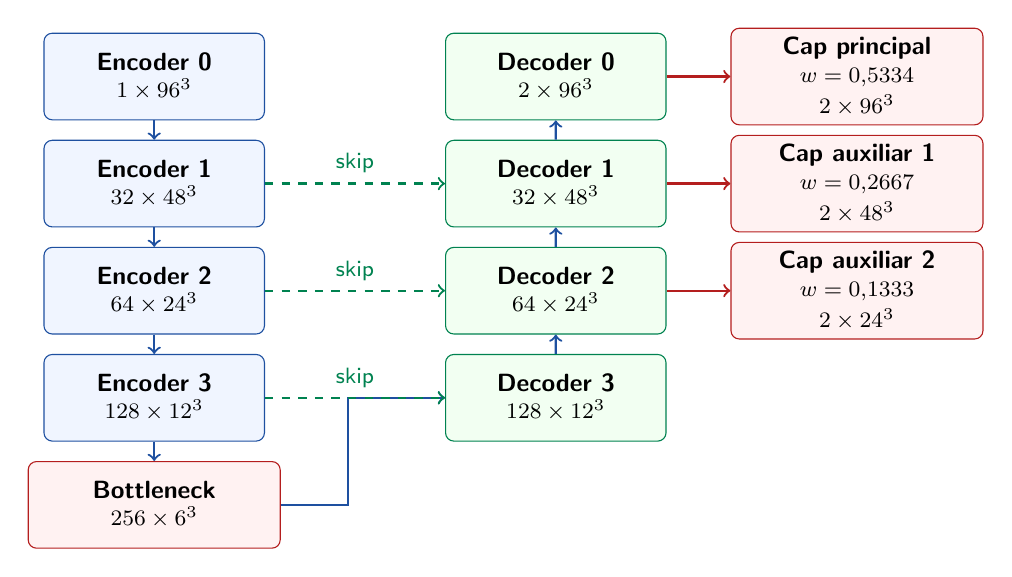
\begin{tikzpicture}[scale=0.85,
    enc/.style={rectangle, rounded corners=3pt, draw=frameblue,
                fill=frametitle, minimum width=2.8cm,
                minimum height=1.1cm, align=center,
                font=\small\bfseries},
    dec/.style={rectangle, rounded corners=3pt, draw=accentgreen,
                fill=green!5, minimum width=2.8cm,
                minimum height=1.1cm, align=center,
                font=\small\bfseries},
    bot/.style={rectangle, rounded corners=3pt, draw=accentred,
                fill=red!5, minimum width=3.2cm,
                minimum height=1.1cm, align=center,
                font=\small\bfseries},
    arr/.style={->, thick, color=frameblue},
    skip/.style={->, dashed, thick, color=accentgreen}]

    % Encoder
    \node[enc] (e0) at (0, 0)   {\shortstack{Encoder 0\\
                                 {\footnotesize $1\times96^3$}}};
    \node[enc] (e1) at (0,-1.6) {\shortstack{Encoder 1\\
                                 {\footnotesize $32\times48^3$}}};
    \node[enc] (e2) at (0,-3.2) {\shortstack{Encoder 2\\
                                 {\footnotesize $64\times24^3$}}};
    \node[enc] (e3) at (0,-4.8) {\shortstack{Encoder 3\\
                                 {\footnotesize $128\times12^3$}}};
    \node[bot] (e4) at (0,-6.4) {\shortstack{Bottleneck\\
                                 {\footnotesize $256\times6^3$}}};

    % Decoder
    \node[dec] (d3) at (6,-4.8) {\shortstack{Decoder 3\\
                                 {\footnotesize $128\times12^3$}}};
    \node[dec] (d2) at (6,-3.2) {\shortstack{Decoder 2\\
                                 {\footnotesize $64\times24^3$}}};
    \node[dec] (d1) at (6,-1.6) {\shortstack{Decoder 1\\
                                 {\footnotesize $32\times48^3$}}};
    \node[dec] (d0) at (6, 0)   {\shortstack{Decoder 0\\
                                 {\footnotesize $2\times96^3$}}};

    % Deep Supervision heads
    \node[bot] (ds0) at (10.5, 0)   {\shortstack{Cap principal\\
                                     {\footnotesize $w=0{,}5334$}\\
                                     {\footnotesize $2\times96^3$}}};
    \node[bot] (ds1) at (10.5,-1.6) {\shortstack{Cap auxiliar 1\\
                                     {\footnotesize $w=0{,}2667$}\\
                                     {\footnotesize $2\times48^3$}}};
    \node[bot] (ds2) at (10.5,-3.2) {\shortstack{Cap auxiliar 2\\
                                     {\footnotesize $w=0{,}1333$}\\
                                     {\footnotesize $2\times24^3$}}};

    % Encoder arrows
    \draw[arr] (e0) -- (e1);
    \draw[arr] (e1) -- (e2);
    \draw[arr] (e2) -- (e3);
    \draw[arr] (e3) -- (e4);

    % Bottleneck to decoder
    \draw[arr] (e4.east) -- ++(1,0) |- (d3.west);

    % Decoder arrows
    \draw[arr] (d3) -- (d2);
    \draw[arr] (d2) -- (d1);
    \draw[arr] (d1) -- (d0);

    % Skip connections
    \draw[skip] (e3.east) -- (d3.west)
        node[midway, above, font=\footnotesize\color{accentgreen}]
        {skip};
    \draw[skip] (e2.east) -- (d2.west)
        node[midway, above, font=\footnotesize\color{accentgreen}]
        {skip};
    \draw[skip] (e1.east) -- (d1.west)
        node[midway, above, font=\footnotesize\color{accentgreen}]
        {skip};

    % Deep supervision arrows
    \draw[arr, color=accentred] (d0.east) -- (ds0.west);
    \draw[arr, color=accentred] (d1.east) -- (ds1.west);
    \draw[arr, color=accentred] (d2.east) -- (ds2.west);
\end{tikzpicture}
\end{center}


% ─────────────────────────────────────────────
\subsection{Input}
% ─────────────────────────────────────────────

Input-ul DynUNet este un patch 3D de dimensiune
$(C_{\text{in}},\, D,\, H,\, W)$, unde $C_{\text{in}}$ reprezintă
numărul de canale de intrare, iar $D$, $H$, $W$ reprezintă
dimensiunile spațiale ale patch-ului (adâncime, înălțime, lățime)
în voxeli. Fiecare voxel conține o valoare scalară normalizată
în intervalul $[0,\,1]$.

\begin{itemize}
    \item $C_{\text{in}}$ — numărul de canale de intrare ale volumului CT
    \item $D$ — adâncimea patch-ului (Depth), măsurată în voxeli
    \item $H$ — înălțimea patch-ului (Height), măsurată în voxeli
    \item $W$ — lățimea patch-ului (Width), măsurată în voxeli
\end{itemize}

% ─────────────────────────────────────────────
\subsection{Convoluția 3D — operația de bază}
% ─────────────────────────────────────────────

Operația fundamentală din DynUNet este convoluția 3D. Fie
$\mathbf{X} \in \mathbb{R}^{C_{\text{in}} \times D \times H \times W}$
tensorul de input și
$\mathbf{W} \in \mathbb{R}^{C_{\text{out}} \times C_{\text{in}}
\times K \times K \times K}$ tensorul de ponderi (kernel).
Output-ul convoluției pe canalul $c_{\text{out}}$ este:

\begin{equation}
    \mathbf{Y}[c_{\text{out}},\, d,\, h,\, w]
    = \sum_{c_{\text{in}}=1}^{C_{\text{in}}}
      \sum_{i,j,k=0}^{K-1}
      \mathbf{W}[c_{\text{out}},\, c_{\text{in}},\, i,\, j,\, k]
      \cdot
      \mathbf{X}[c_{\text{in}},\;
                 d{\cdot}S+i,\;
                 h{\cdot}S+j,\;
                 w{\cdot}S+k]
\end{equation}

\begin{itemize}
    \item $C_{\text{in}}$ — numărul de canale de intrare
    \item $C_{\text{out}}$ — numărul de canale de ieșire
    \item $K$ — dimensiunea kernelului de convoluție
    \item $S$ — stride-ul convoluției
    \item $d, h, w$ — indicii spațiali ai voxelului de output
    \item $i, j, k$ — indicii locali în fereastra kernelului
\end{itemize}

Kernelul $K \times K \times K$ cu stride $S$ realizează simultan
două operații: extragerea de trăsături locale prin ponderile
$\mathbf{W}$ antrenabile și, atunci când $S > 1$, downsampling
spațial prin saltul de $S$ voxeli la fiecare pas.

Dimensiunea spațială după convoluție se calculează astfel:

\begin{equation}
    D_{\text{out}}
    = \left\lfloor \frac{D_{\text{in}} - K + 2P}{S}
      \right\rfloor + 1
\end{equation}

\begin{itemize}
    \item $D_{\text{in}}$ — dimensiunea spațială a intrării
    \item $D_{\text{out}}$ — dimensiunea spațială a ieșirii
    \item $P$ — padding-ul aplicat înainte de convoluție
    \item $S$ — stride-ul convoluției
\end{itemize}


Spre exemplu, pentru kernel $K=3$, padding $P=1$ și stride $S=2$,
formula se simplifică la
$D_{\text{out}} = \lfloor D_{\text{in}} / 2 \rfloor$,
înjumătățind dimensiunea spațială la fiecare nivel de downsampling:

    

% ─────────────────────────────────────────────
\subsection{Residual Block}
% ─────────────────────────────────────────────

Fiecare nivel al encoder-ului și decoder-ului conține blocuri
reziduale, inspirate din ResNet~\cite{he2016resnet}. Un residual
block aplică o transformare $\mathcal{F}$ asupra input-ului
$\mathbf{x}$, adăugând la final input-ul original prin
shortcut connection:

\begin{equation}
    \mathbf{y} = \mathcal{F}(\mathbf{x},\,\{\mathbf{W}_i\})
               + \mathbf{x}
\end{equation}

\begin{itemize}
    \item $\mathbf{x}$ — tensorul de input al blocului
    \item $\mathbf{y}$ — tensorul de output al blocului
    \item $\mathcal{F}(\mathbf{x},\{\mathbf{W}_i\})$ — transformarea reziduală aplicată lui $\mathbf{x}$
    \item $\{\mathbf{W}_i\}$ — ponderile antrenabile ale blocului
    \item $+\,\mathbf{x}$ — shortcut connection (identity mapping)
\end{itemize}


Transformarea reziduală $\mathcal{F}$ constă dintr-o secvență de
normalizare, activare și convoluție, aplicată de două ori:

\[
    \mathcal{F}(\mathbf{x}) :
    \underbrace{\text{IN} \to \text{LeakyReLU} \to
    \text{Conv3D}}_{\text{primul strat}}
    \to
    \underbrace{\text{IN} \to \text{LeakyReLU} \to
    \text{Conv3D}}_{\text{al doilea strat}}
\]

\textbf{De ce IN $\to$ LeakyReLU $\to$ Conv și nu invers?}
Ordinea \textit{pre-activation} (normalizare și activare înainte
de convoluție) permite gradienților să curgă direct prin shortcut
fără a traversa funcții nelineare — convergență mai rapidă și
antrenament mai stabil față de ordinea clasică post-activation.

\begin{center}
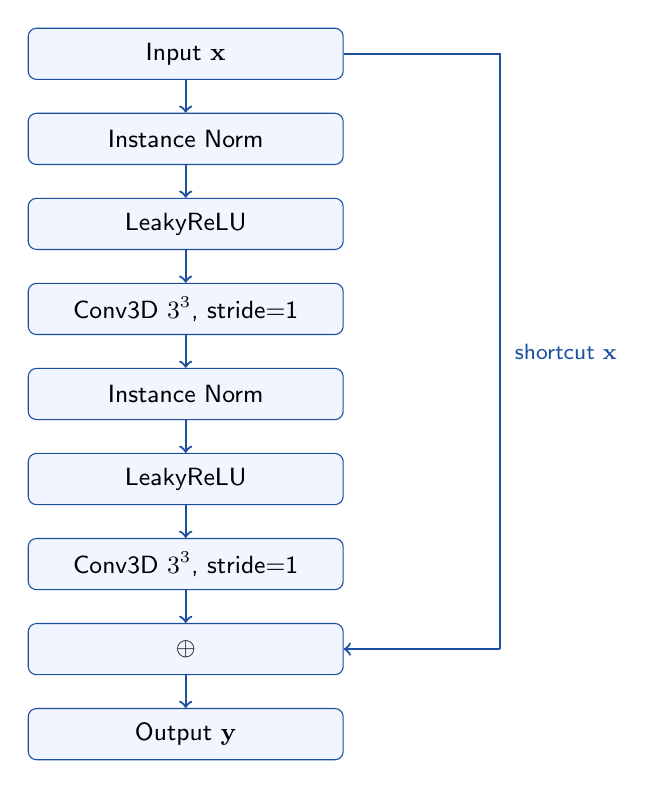
\begin{tikzpicture}[scale=0.9,
    blk/.style={rectangle, rounded corners=3pt, draw=frameblue,
                fill=frametitle, minimum width=4cm,
                minimum height=0.65cm, align=center, font=\small},
    arr/.style={->, thick, color=frameblue}]

    \node[blk] (in)  at (0, 0)   {Input $\mathbf{x}$};
    \node[blk] (in1) at (0,-1.2) {Instance Norm};
    \node[blk] (r1)  at (0,-2.4) {LeakyReLU};
    \node[blk] (c1)  at (0,-3.6) {Conv3D $3^3$, stride=1};
    \node[blk] (in2) at (0,-4.8) {Instance Norm};
    \node[blk] (r2)  at (0,-6.0) {LeakyReLU};
    \node[blk] (c2)  at (0,-7.2) {Conv3D $3^3$, stride=1};
    \node[blk] (add) at (0,-8.4) {$\oplus$};
    \node[blk] (out) at (0,-9.6) {Output $\mathbf{y}$};

    \draw[arr] (in)  -- (in1);
    \draw[arr] (in1) -- (r1);
    \draw[arr] (r1)  -- (c1);
    \draw[arr] (c1)  -- (in2);
    \draw[arr] (in2) -- (r2);
    \draw[arr] (r2)  -- (c2);
    \draw[arr] (c2)  -- (add);
    \draw[arr] (add) -- (out);

    \draw[color=frameblue, thick]
    (in.east) -- ++(2.2,0) coordinate (tr)
               -- ++(0,-8.4) coordinate (br);
\draw[->, color=frameblue, thick] (br) -- (add.east);
\node[right=2pt, font=\footnotesize, color=frameblue]
    at ($(tr)!0.5!(br)$) {shortcut $\mathbf{x}$};

\end{tikzpicture}
\end{center}

Importanța shortcut-ului este fundamentală pentru antrenarea
rețelelor adânci. Gradientul pierderii față de input-ul blocului
se descompune în două căi:

\begin{equation}
    \frac{\partial \mathcal{L}}{\partial \mathbf{x}}
    = \frac{\partial \mathcal{L}}{\partial \mathbf{y}}
      \cdot \left(1 + \frac{\partial \mathcal{F}}
                            {\partial \mathbf{x}}\right)
\end{equation}

\begin{itemize}
    \item $\frac{\partial \mathcal{L}}{\partial \mathbf{x}}$ — gradientul pierderii față de input-ul blocului
    \item $\frac{\partial \mathcal{L}}{\partial \mathbf{y}}$ — gradientul pierderii față de output-ul blocului
    \item $\frac{\partial \mathcal{F}}{\partial \mathbf{x}}$ — contribuția căii reziduale
    \item $1$ — termenul shortcut, garantează gradient nenul
\end{itemize}


Termenul $1$ garantează că gradientul nu se stinge indiferent de
adâncimea rețelei: chiar dacă
$\frac{\partial \mathcal{F}}{\partial \mathbf{x}} \approx 0$,
gradientul rămâne $\frac{\partial \mathcal{L}}{\partial \mathbf{y}}$,
prevenind fenomenul de vanishing gradients.


% ─────────────────────────────────────────────
\subsection{Instance Normalization}
% ─────────────────────────────────────────────

Instance Normalization (IN) normalizează fiecare canal al unui
exemplu individual, independent de restul batch-ului:

\begin{equation}
    \text{IN}(x_c)
    = \frac{x_c - \mu_c}{\sqrt{\sigma_c^2 + \varepsilon}}
\end{equation}

\begin{itemize}
    \item $x_c$ — valorile voxelilor pe canalul $c$
    \item $\mu_c$ — media valorilor pe canalul $c$ al unui singur volum
    \item $\sigma_c^2$ — varianța valorilor pe canalul $c$ al unui singur volum
    \item $\varepsilon$ — termen de stabilitate numerică, previne împărțirea la zero
\end{itemize}


Față de Batch Normalization (BN), care calculează statistici pe
întreg batch-ul, IN calculează statistici per volum, independent
de ceilalți:

\begin{center}
\begin{tabular}{lcc}
    \toprule
    & \textbf{Batch Normalization} & \textbf{Instance Normalization} \\
    \midrule
    Statistici calculate pe & Întregul batch  & Un singur volum \\
    Funcționare la batch=1  & Instabilă       & Corectă \\
    Funcționare la batch=2  & Zgomotoasă      & Corectă \\
    Dependență între volume & Da              & Nu \\
    Utilizare recomandată   & Clasificare 2D  & Segmentare medicală 3D \\
    \bottomrule
\end{tabular}
\end{center}

Spre exemplu, la \texttt{batch\_size=2} cu patch-uri de $96^3$
voxeli, BN calculează statistici pe doar 2 volume — insuficient
pentru estimări stabile. IN calculează statistici independent
pe fiecare din cele 2 volume, producând rezultate corecte
indiferent de dimensiunea batch-ului.

% ─────────────────────────────────────────────
\subsection{Encoder}
% ─────────────────────────────────────────────

Encoder-ul reduce progresiv rezoluția spațială a volumului,
crescând simultan numărul de canale (feature maps). La fiecare
nivel de downsampling, convoluția cu stride $S$ reduce 
dimensiunile spațiale cu factorul $S$  , în timp ce numărul de canale crește,
menținând capacitatea informațională totală aproximativ constantă.

Câmpul receptiv efectiv  (totalitatea voxelilor din input care influenteaza valoarea unui neuron)  crește cu adâncimea rețelei: la primul
nivel, fiecare neuron procesează o regiune locală de
$K \times K \times K$ voxeli, determinată de dimensiunea
kernelului. Pe măsură ce feature map-urile sunt downsample-uite
la nivelurile următoare, neuronii de la niveluri mai adânci
„văd" regiuni din ce în ce mai mari din volumul original.
La nivelul bottleneck, câmpul receptiv poate acoperi o porțiune
semnificativă din patch, permițând modelului să capteze context
anatomic la scară largă.


Spre exemplu, pentru un patch de $96 \times 96 \times 96$
voxeli cu 5 niveluri și kerneluri $3\times3\times3$:

\begin{center}
\begin{tabular}{cccccc}
    \toprule
    \textbf{Nivel} & \textbf{Operație} & \textbf{Kernel} &
    \textbf{Stride} & \textbf{Dimensiune} & \textbf{Canale} \\
    \midrule
    0 & Conv + ResBlock & $3^3$ & 1 & $96^3$ & $1   \to 32$  \\
    1 & Conv + ResBlock & $3^3$ & 2 & $48^3$ & $32  \to 64$  \\
    2 & Conv + ResBlock & $3^3$ & 2 & $24^3$ & $64  \to 128$ \\
    3 & Conv + ResBlock & $3^3$ & 2 & $12^3$ & $128 \to 256$ \\
    4 & Conv + ResBlock & $3^3$ & 2 & $6^3$  & $256 \to 256$ \\
    \bottomrule
\end{tabular}
\end{center}
\begin{itemize}
    \item \textbf{Nivelul 0:} inputul are 1 canal (volumul CT) ---
    după convoluție rezultă 32 de feature maps, fiecare detectând
    un pattern local distinct din volum.
    \item \textbf{Nivelul 1:} cele 32 de feature maps devin input
    --- produc 64 de feature maps mai abstracte, la o rezoluție
    spațială înjumătățită ($48^3$).
    \item Pe măsură ce adâncimea crește, feature maps-urile devin
    tot mai abstracte: de la muchii și texturi locale la structuri
    anatomice complexe (contur ficat, tumoră).
\end{itemize}


% ─────────────────────────────────────────────
\subsection{Skip Connections și Decoder}
% ─────────────────────────────────────────────
Decoder-ul reconstruiește progresiv rezoluția spațială prin
convoluții transpuse cu stride $S$, inversând operația de
downsampling aplicată de encoder. La fiecare nivel, convoluția
transpusă înmulțește dimensiunile spațiale ale feature maps-urilor cu termenul $S$,
fără a recupera informația pierdută prin downsampling — aceasta
este compensată prin skip connections, care transferă direct
feature maps de la nivelul corespunzător al encoder-ului.
Concatenarea celor două surse de informație permite decoder-ului
să combine contextul semantic capturat la rezoluții mici cu
detaliile spațiale fine păstrate de encoder.



\begin{equation}
    \mathbf{D}_l
    = \text{Conv3D}\!\bigl([\,\mathbf{U}_l \;\|\; \mathbf{E}_l\,]\bigr)
\end{equation}

\begin{itemize}
    \item $\mathbf{D}_l$ — feature maps output la nivelul $l$ al decoder-ului
    \item $\mathbf{U}_l$ — feature maps upsamplate din nivelul $l+1$
    \item $\mathbf{E}_l$ — feature maps din encoder la nivelul $l$, transmise via skip connection
    \item $[\cdot\|\cdot]$ — concatenare pe dimensiunea canalelor
\end{itemize}




Spre exemplu, la nivelul 1 al decoder-ului, feature maps
upsamplate ($64 \times 48^3$) sunt concatenate cu feature maps
din Encoder 1 ($32 \times 48^3$), producând un tensor de
$96 \times 48^3$ canale care combină informația globală
cu detaliile spațiale fine:

\begin{center}
\begin{tabular}{cccc}
    \toprule
    \textbf{Nivel decoder} & \textbf{Din encoder} &
    \textbf{Upsampled} & \textbf{După concatenare} \\
    \midrule
    3 & $128 \times 12^3$ & $256 \times 12^3$ & $384 \times 12^3$ \\
    2 & $64  \times 24^3$ & $128 \times 24^3$ & $192 \times 24^3$ \\
    1 & $32  \times 48^3$ & $64  \times 48^3$ & $96  \times 48^3$ \\
    \bottomrule
\end{tabular}
\end{center}




\begin{center}
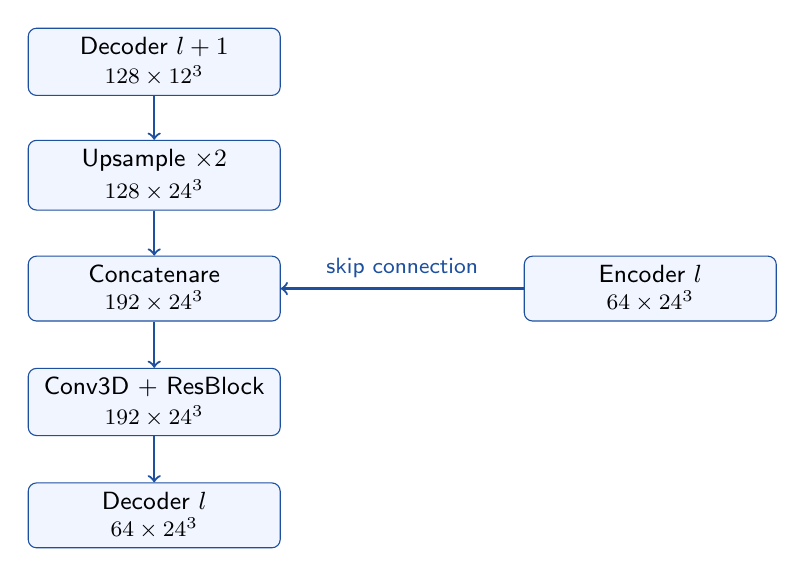
\begin{tikzpicture}[scale=0.9,
    blk/.style={rectangle, rounded corners=3pt, draw=frameblue,
                fill=frametitle, minimum width=3.2cm,
                minimum height=0.8cm, align=center, font=\small},
    arr/.style={->, thick, color=frameblue},
    sarr/.style={->, thick, color=frameblue}]

    % Coloana principala
    \node[blk] (prev) at (0, 0)   {\shortstack{Decoder $l+1$\\
                                   {\footnotesize $128\times12^3$}}};
    \node[blk] (up)   at (0,-1.6) {\shortstack{Upsample $\times2$\\
                                   {\footnotesize $128\times24^3$}}};
    \node[blk] (cat)  at (0,-3.2) {\shortstack{Concatenare\\
                                   {\footnotesize $192\times24^3$}}};
    \node[blk] (conv) at (0,-4.8) {\shortstack{Conv3D + ResBlock\\
                                   {\footnotesize $192\times24^3$}}};
    \node[blk] (out)  at (0,-6.4) {\shortstack{Decoder $l$\\
                                   {\footnotesize $64\times24^3$}}};

    % Skip connection
    \node[blk] (enc) at (7,-3.2)  {\shortstack{Encoder $l$\\
                                   {\footnotesize $64\times24^3$}}};

    % Sageti principale
    \draw[arr] (prev) -- (up);
    \draw[arr] (up)   -- (cat);
    \draw[arr] (cat)  -- (conv);
    \draw[arr] (conv) -- (out);

    % Sageata skip
    \draw[sarr] (enc.west) -- (cat.east)
        node[midway, above, font=\footnotesize, color=frameblue]
        {skip connection};

\end{tikzpicture}
\end{center}



% ─────────────────────────────────────────────
\subsection{Deep Supervision}
% ─────────────────────────────────────────────

Deep supervision atașează capete de clasificare intermediare la
nivelurile superioare ale decoder-ului, producând output-uri
simultane la rezoluții diferite. Fiecare output intermediar este
comparat cu ground truth-ul downsamplat la rezoluția
corespunzătoare, iar contribuțiile sunt însumate cu ponderi
descrescătoare:

\begin{equation}
    \mathcal{L}_{\text{total}}
    = \sum_{k=0}^{K} \hat{w}_k \cdot
      \mathcal{L}\!\left(O_k,\; y_{/2^k}\right)
\end{equation}

\begin{itemize}
    \item $K$ — numărul total de capete de output
    \item $k$ — indicele capului ($k=0$ = capul principal)
    \item $\hat{w}_k$ — ponderea renormalizată a capului $k$
    \item $O_k$ — output-ul la rezoluția capului $k$
    \item $y_{/2^k}$ — ground truth downsamplat la rezoluția capului $k$
\end{itemize}


Avantajul principal este că gradienții ajung direct la straturile
intermediare ale decoder-ului fără să traverseze straturile
superioare, combătând vanishing gradients și accelerând convergența
în primele epoci de antrenament.

Spre exemplu, cu \texttt{deep\_supr\_num=2} sunt produse
3 output-uri cu ponderi descrescătoare:

\begin{center}
\begin{tabular}{cccc}
    \toprule
    \textbf{Cap} & \textbf{Rezoluție} &
    \textbf{Pondere inițială} & \textbf{Pondere renormalizată} \\
    \midrule
    $O_0$ (principal) & $96^3$ & $0{,}5334$ & $\approx 0{,}5715$ \\
    $O_1$ (auxiliar)  & $48^3$ & $0{,}2667$ & $\approx 0{,}2858$ \\
    $O_2$ (auxiliar)  & $24^3$ & $0{,}1333$ & $\approx 0{,}1428$ \\
    \bottomrule
\end{tabular}
\end{center}

% ─────────────────────────────────────────────
\subsection{Output}
% ─────────────────────────────────────────────

Output-ul DynUNet este un tensor de forma
$(B,\, C_{\text{out}},\, D,\, H,\, W)$, unde $B$ este batch
size-ul, $C_{\text{out}}$ este numărul de clase de output,
iar $D \times H \times W$ sunt dimensiunile spațiale ale
patch-ului. Fiecare canal conține logits (valori nenormalizate)
pentru clasa corespunzătoare.

Masca de segmentare finală se obține prin aplicarea softmax
pe dimensiunea canalelor, urmată de $\arg\max$:

\begin{equation}
    \hat{y}_{d,h,w}
    = \arg\max_{c}
      \frac{e^{O_0[c,\,d,\,h,\,w]}}
           {\displaystyle\sum_{c'}
            e^{O_0[c',\,d,\,h,\,w]}}
\end{equation}

Spre exemplu, pentru segmentarea ficatului cu
$C_{\text{out}}=2$ clase (fundal și ficat), dacă modelul
produce logits $[-1{,}2;\; 3{,}4]$ pentru un voxel, după
softmax se obțin probabilitățile $[0{,}008;\; 0{,}992]$,
iar $\arg\max$ atribuie voxelul clasei \textit{ficat}.






% ────────────────────────────────────────────────────────────────────────────
\section{SwinUNETR}
% ────────────────────────────────────────────────────────────────────────────

SwinUNETR (Swin Transformer UNETR) combină puterea de reprezentare globală a
Transformer-elor cu structura encoder-decoder a UNet, adaptată pentru volume
medicale 3D. Arhitectura a fost propusă de Tang et al.\ (2022) și reprezintă
una dintre cele mai performante arhitecturi pentru segmentarea medicală volumetrică.


\subsection{Patch Partition și Linear Embedding}

Primul pas al encoder-ului Swin este împărțirea volumului de input
în tokeni 3D. Volumul de intrare $\mathbf{X} \in \mathbb{R}^{C_{in}
\times D \times H \times W}$ este partitionat în cuburi non-overlapping
de $2\times2\times2$ voxeli. Fiecare cub devine un token prin
concatenarea valorilor tuturor voxelilor din toate canalele:

\formula{
    \text{token}_{d,h,w} = \text{flatten}\!\left(\mathbf{X}[:,\,
    2d:2d+2,\, 2h:2h+2,\, 2w:2w+2]\right)
    \in \mathbb{R}^{8 \cdot C_{in}}
}

\begin{itemize}
    \item $\mathbf{X}[:,\, 2d:2d+2,\, 2h:2h+2,\, 2w:2w+2]$ ---
    extrage cubul de $2\times2\times2$ voxeli de la poziția $(d,h,w)$,
    pe toate cele $C_{in}$ canale, rezultând un sub-volum de formă
    $C_{in} \times 2 \times 2 \times 2$
    \item $\text{flatten}(\cdot)$ --- aplatizează sub-volumul
    $C_{in} \times 2 \times 2 \times 2$ într-un vector 1D de lungime
    $8 \cdot C_{in}$
    \item $8 \cdot C_{in}$ --- dimensiunea tokenului: 8 poziții
    spațiale ($2\times2\times2$) înmulțite cu numărul de canale
\end{itemize}

Spre exemplu, pentru $C_{in} = 1$ (volum CT monocanal), fiecare
token conține $8 \times 1 = 8$ valori — intensitățile HU ale celor
8 voxeli ai cubului.

Tokenii rezultați sunt proiectați printr-un strat liniar (Linear
Embedding) în spațiul de reprezentare de dimensiune
\texttt{feature\_size}:

\formula{
    \mathbf{t}_{d,h,w} = \mathbf{W}_{\text{emb}} \cdot
    \text{token}_{d,h,w} + \mathbf{b}_{\text{emb}},
    \qquad \mathbf{W}_{\text{emb}} \in \mathbb{R}^{\texttt{feature\_size} \times 8 C_{in}}
}

\begin{itemize}
    \item $\text{token}_{d,h,w} \in \mathbb{R}^{8 C_{in}}$ ---
    vectorul brut al tokenului, obținut prin flatten
    \item $\mathbf{W}_{\text{emb}} \in \mathbb{R}^{\texttt{feature\_size} \times 8 C_{in}}$
    --- matricea de ponderi a stratului liniar, care transformă fiecare
    token din $8 C_{in}$ valori brute în \texttt{feature\_size} features abstracte
    \item $\mathbf{b}_{\text{emb}} \in \mathbb{R}^{\texttt{feature\_size}}$ --- bias-ul
    stratului liniar
    \item $\mathbf{t}_{d,h,w} \in \mathbb{R}^{\texttt{feature\_size}}$ --- embedding-ul
    final al tokenului, reprezentat ca vector de \texttt{feature\_size} features
\end{itemize}

Scopul Linear Embedding este de a aduce toți tokenii într-un spațiu
comun de \texttt{feature\_size} features, indiferent de numărul de
canale de intrare. Practic, stratul liniar învață o reprezentare
compactă și densă a fiecărui cub de $2\times2\times2$ voxeli,
pregătind tokenii pentru procesarea ulterioară de către blocurile
Swin Transformer.

Dintr-un volum de $D \times H \times W$ voxeli rezultă
$\frac{D}{2} \times \frac{H}{2} \times \frac{W}{2}$ tokeni, fiecare
reprezentat ca vector de \texttt{feature\_size} features. Spre exemplu,
pentru un patch de $96\times96\times96$ voxeli rezultă
$48\times48\times48 = 110\,592$ tokeni.



\subsection{Window Multi-Head Self-Attention (W-MSA)}

Mecanismul de atenție determină, pentru fiecare token, cât de mult
trebuie să „acorde atenție" celorlalți tokeni din vecinătatea sa —
cu alte cuvinte, care tokeni sunt relevanți pentru reprezentarea sa.
În ViT clasic, fiecare token interacționează cu toți ceilalți tokeni
din volum (atenție globală), ceea ce duce la o complexitate
$O(n^2)$ în numărul de tokeni — impracticabil pentru volume 3D mari
unde $n$ poate ajunge la sute de mii de tokeni.


\textbf{Soluția Swin:} tokenii sunt grupați în ferestre locale 3D de dimensiune
$w \times w \times w$ tokeni. Atenția se calculează \textit{doar în interiorul
ferestrelor}, reducând complexitatea:

\formula{
    \text{Complexitate W-MSA} = \frac{n}{w^3} \cdot (w^3)^2 / w^3 = n \cdot w^3 = O(n)
}
\formula{
    \text{Complexitate globală} = n^2 = O(n^2)
}


\textbf{Calculul atenției:} pentru fiecare token $\mathbf{t}_i$ dintr-o fereastră,
se calculează trei vectori prin proiecții liniare:

\formula{
    Q_i = \mathbf{t}_i \mathbf{W}_Q, \quad
    K_j = \mathbf{t}_j \mathbf{W}_K, \quad
    V_j = \mathbf{t}_j \mathbf{W}_V
}

\begin{itemize}
    \item $Q_i$ (\textbf{Query}) — „Ce informație caut?" — vectorul de interogare al tokenului $i$
    \item $K_j$ (\textbf{Key}) — „Ce informație ofer?" — vectorul cheie al tokenului $j$
    \item $V_j$ (\textbf{Value}) — „Ce informație transfer?" — vectorul valoare al tokenului $j$
\end{itemize}

Scorul de atenție dintre tokenii $i$ și $j$ din aceeași fereastră
măsoară cât de mult trebuie tokenul $i$ să „acorde atenție"
tokenului $j$. Se calculează prin produsul scalar dintre vectorul
Query al lui $i$ și vectorul Key al lui $j$, la care se adaugă
un bias de poziție relativă:

\formula{
    \text{Attention}(Q, K, V) = \text{softmax}\!\left(
    \frac{QK^T}{\sqrt{d_k}} + B\right) V
}

\begin{itemize}
    \item $QK^T$ --- produsul scalar dintre toți vectorii Query și
    Key din fereastră, producând o matrice de scoruri de formă
    $w^3 \times w^3$ — scorul dintre fiecare pereche de tokeni
    \item $\sqrt{d_k}$ --- factor de scalare care previne valori
    prea mari ale produsului scalar, care ar împinge funcția
    softmax în zone cu gradient mic
    \item $B$ --- \textbf{Relative Position Bias}: un bias
    antrenabil $B_{ij}$ adăugat scorului dintre tokenii $i$ și $j$,
    care codifică distanța relativă dintre ei în interiorul
    ferestrei. Transformer-ul nu are noțiune nativă de poziție
    spațială — fără acest bias, tokenii de la marginea ferestrei
    și cei din centru ar fi tratați identic, indiferent de distanța
    dintre ei
    \item $\text{softmax}(\cdot)$ --- normalizează scorurile în
    probabilități între 0 și 1, astfel încât suma atenției acordate
    tuturor tokenilor din fereastră să fie 1
    \item $V$ --- înmulțirea cu vectorii Value produce reprezentarea
    finală: o medie ponderată a informației din toți tokenii
    ferestrei, unde ponderile sunt scorurile de atenție
\end{itemize}

\textbf{Multi-Head Attention.}
În loc să calculeze un singur set de scoruri de atenție,
Multi-Head Attention calculează $h$ seturi independente în paralel
— numite \textit{capete} (heads). Fiecare cap lucrează pe un
sub-spațiu diferit al reprezentării, de dimensiune
$d_k = \texttt{feature\_size} / h$:

\formula{
    \text{MultiHead}(Q,K,V) =
    \text{Concat}(\text{head}_1, \ldots, \text{head}_h)\,\mathbf{W}_O,
    \qquad \mathbf{W}_O \in \mathbb{R}^{\texttt{feature\_size}
    \times \texttt{feature\_size}}
}

\begin{itemize}
    \item $\text{head}_m = \text{Attention}(Q\mathbf{W}_Q^m,\,
    K\mathbf{W}_K^m,\, V\mathbf{W}_V^m)$ --- al $m$-lea cap de
    atenție, care folosește propriile sale matrice de proiecție
    $\mathbf{W}_Q^m, \mathbf{W}_K^m, \mathbf{W}_V^m$
    \item $\text{Concat}(\cdot)$ --- concatenarea outputurilor
    tuturor capetelor, producând un vector de dimensiune
    $h \cdot d_k = \texttt{feature\_size}$
    \item $\mathbf{W}_O$ --- o proiecție liniară finală care
    combină informația din toate capetele într-o singură
    reprezentare de dimensiune \texttt{feature\_size}
\end{itemize}

Motivul pentru care se folosesc mai multe capete este că fiecare
cap poate învăța să fie atent la aspecte diferite ale volumului
în același timp: un cap poate captura relații locale de textură,
altul poate detecta contururi, iar altul poate integra context
anatomic la distanță mare. Rezultatul final combină toate aceste
perspective într-o singură reprezentare.


\subsection{Shifted Window Attention (SW-MSA)}

\textbf{Problema W-MSA:} tokenii din ferestre diferite nu comunică niciodată.
Un token de la granița ferestrei A și unul de la granița ferestrei B adiacente
sunt vecini fizici în imagine, dar nu interacționează prin atenție.

\textbf{Soluția:} la fiecare al doilea bloc Swin, ferestrele sunt deplasate
(shifted) cu $\lfloor w/2 \rfloor$ tokeni pe fiecare axă. Această deplasare
forțează tokenii de la granițele fostelor ferestre să ajungă în aceeași fereastră
nouă, permițând comunicarea între ferestre adiacente.

\begin{center}
\begin{tabular}{cc}
\textbf{Layer 1 — W-MSA (ferestre normale)} &
\textbf{Layer 2 — SW-MSA (ferestre shiftate)} \\[6pt]
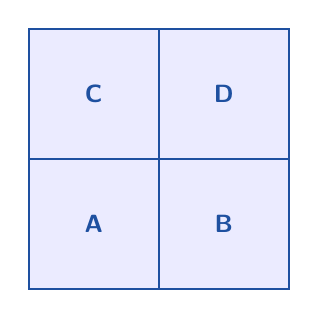
\begin{tikzpicture}[scale=0.55]
    \draw[thick, frameblue, fill=blue!8] (0,0) rectangle (3,3);
    \draw[thick, frameblue, fill=blue!8] (3,0) rectangle (6,3);
    \draw[thick, frameblue, fill=blue!8] (0,3) rectangle (3,6);
    \draw[thick, frameblue, fill=blue!8] (3,3) rectangle (6,6);
    \node[font=\small\bfseries\color{frameblue}] at (1.5,1.5) {A};
    \node[font=\small\bfseries\color{frameblue}] at (4.5,1.5) {B};
    \node[font=\small\bfseries\color{frameblue}] at (1.5,4.5) {C};
    \node[font=\small\bfseries\color{frameblue}] at (4.5,4.5) {D};
\end{tikzpicture}
&
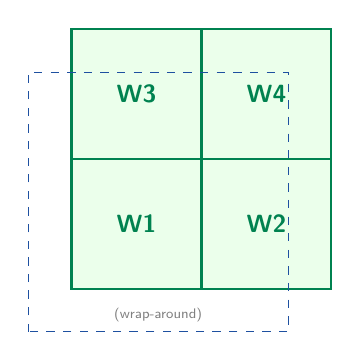
\begin{tikzpicture}[scale=0.55]
    \draw[thick, accentgreen, fill=green!8] (1,1) rectangle (4,4);
    \draw[thick, accentgreen, fill=green!8] (4,1) rectangle (7,4);
    \draw[thick, accentgreen, fill=green!8] (1,4) rectangle (4,7);
    \draw[thick, accentgreen, fill=green!8] (4,4) rectangle (7,7);
    \draw[dashed, frameblue] (0,0) rectangle (6,6);
    \node[font=\small\bfseries\color{accentgreen}] at (2.5,2.5) {W1};
    \node[font=\small\bfseries\color{accentgreen}] at (5.5,2.5) {W2};
    \node[font=\small\bfseries\color{accentgreen}] at (2.5,5.5) {W3};
    \node[font=\small\bfseries\color{accentgreen}] at (5.5,5.5) {W4};
    \node[font=\tiny\color{gray}] at (3,0.4) {(wrap-around)};
\end{tikzpicture}
\end{tabular}
\end{center}

Fereastra W1 conține acum tokeni din fostele ferestre A, B, C și D. La fiecare
două straturi (W-MSA + SW-MSA), fiecare token a interacționat cu vecinii săi
din toate ferestrele adiacente.

\textbf{Attention Mask:}
după deplasare, unele ferestre conțin tokeni care fizic nu sunt vecini
în imaginea originală (prin wrap-around). O \textbf{mască de atenție} blochează
comunicarea între tokenii non-vecini prin adăugarea valorii $-\infty$ la scorul
de atenție, care devine 0 după softmax, anulând complet influența acestora.

\subsection{Swin Transformer Block}

Un bloc Swin procesează tokenii în două etape succesive: mai întâi
prin mecanismul de atenție, apoi printr-o rețea feed-forward. Ambele
etape folosesc conexiuni reziduale (shortcut), similar cu ResNet,
pentru a preveni vanishing gradients.

\paragraph{Etapa 1 — W-MSA cu Layer Normalization.}
Înainte de atenție, tokenii sunt normalizați prin Layer Normalization
(LN), apoi trec prin W-MSA, iar rezultatul este adunat cu inputul
original prin shortcut connection:

\formula{
    \hat{\mathbf{z}}^l = \text{W-MSA}\!\left(\text{LN}(\mathbf{z}^{l-1})\right) + \mathbf{z}^{l-1}
}

\begin{itemize}
    \item $\mathbf{z}^{l-1}$ --- tokenii de la intrarea blocului $l$
    \item $\text{LN}(\cdot)$ --- Layer Normalization aplicată
    \textit{înainte} de atenție (pre-norm), care normalizează
    fiecare token independent, stabilizând antrenamentul în rețele
    profunde
    \item $\text{W-MSA}(\cdot)$ --- mecanismul de atenție în
    ferestre locale, descris în secțiunea anterioară
    \item $+ \mathbf{z}^{l-1}$ --- shortcut connection: adună
    inputul original la output, garantând că gradientul nu se
    stinge prin adâncimea rețelei
    \item $\hat{\mathbf{z}}^l$ --- tokenii după etapa de atenție
\end{itemize}

\paragraph{Etapa 2 — MLP Feed-Forward.}
Tokenii rezultați din atenție trec printr-un MLP cu două straturi,
aplicat independent pentru fiecare token. Și această etapă folosește
pre-norm și shortcut connection:

\formula{
    \mathbf{z}^l = \text{MLP}\!\left(\text{LN}(\hat{\mathbf{z}}^l)\right) + \hat{\mathbf{z}}^l
}

MLP-ul are structura:

\formula{
    \text{MLP}(\mathbf{t}) = \mathbf{W}_2 \cdot \text{GELU}(\mathbf{W}_1 \mathbf{t} + \mathbf{b}_1) + \mathbf{b}_2
}

\begin{itemize}
    \item $\mathbf{W}_1 \in \mathbb{R}^{4\,\texttt{feature\_size}
    \times \texttt{feature\_size}}$ --- primul strat liniar, care
    extinde reprezentarea fiecărui token de 4 ori
    \item $\text{GELU}(\cdot)$ --- funcția de activare, preferată
    față de ReLU deoarece are gradient non-zero și pentru valori
    negative mici, facilitând antrenamentul
    \item $\mathbf{W}_2 \in \mathbb{R}^{\texttt{feature\_size}
    \times 4\,\texttt{feature\_size}}$ --- al doilea strat liniar,
    care comprimă reprezentarea înapoi la dimensiunea
    \texttt{feature\_size}
\end{itemize}

Rolul MLP-ului este de a introduce transformări non-liniare
independente per token — în timp ce atenția permite comunicarea
între tokeni, MLP-ul rafinează reprezentarea fiecărui token
individual.

\paragraph{Blocuri alternante W-MSA și SW-MSA.}
Blocurile Swin alternează între W-MSA (ferestre fixe) și SW-MSA
(ferestre deplasate cu $\lfloor w/2 \rfloor$ tokeni pe fiecare
axă). Această alternanță este necesară deoarece W-MSA calculează
atenția doar în interiorul ferestrelor — tokenii de la marginile
ferestrelor adiacente nu interacționează niciodată. SW-MSA
rezolvă această problemă prin deplasarea ferestrelor, permițând
comunicarea între toate regiunile volumului:

\formula{
    \hat{\mathbf{z}}^{l+1} = \text{SW-MSA}\!\left(\text{LN}(\mathbf{z}^l)\right) + \mathbf{z}^l
}
\formula{
    \mathbf{z}^{l+1} = \text{MLP}\!\left(\text{LN}(\hat{\mathbf{z}}^{l+1})\right) + \hat{\mathbf{z}}^{l+1}
}

\subsection{Patch Merging și Cele 4 Stagii}

Între stagiile encoder-ului, \textbf{Patch Merging} reduce rezoluția spațială
și crește dimensiunea embedding-ului. Patch Merging concatenează 8 tokeni vecini
($2\times2\times2$) și aplică o proiecție liniară:

\formula{
    \mathbf{t}_{\text{merged}} = \mathbf{W}_{\text{merge}} \cdot
    \text{concat}(\mathbf{t}_{d,h,w},\, \mathbf{t}_{d+1,h,w},\, \ldots,\, \mathbf{t}_{d+1,h+1,w+1})
    \in \mathbb{R}^{2F}
}

Encoder-ul Swin are 4 stagii ierarhice cu rezoluție spațială descrescătoare și
număr de canale crescător ($F \to 2F \to 4F \to 8F$). La ultimul stagiu, câmpul
receptiv efectiv acoperă întregul volum de input, oferind context anatomic global.

\subsection{Preantrenare Self-Supervised (SSL)}

Encoder-ul Swin poate fi preantrenat self-supervised pe volume CT și MRI publice,
folosind un obiectiv de tip \textbf{Masked Volume Inpainting}:

\begin{enumerate}
    \item Se maschează aleatoriu \textbf{75\% din tokenii} volumului de input
    \item Rețeaua trebuie să \textbf{reconstruiască} valorile voxelilor mascați
          din contextul tokenilor nemascați
    \item Loss-ul de preantrenare este $\ell_1$ între valorile reconstruite și cele originale
\end{enumerate}

Similar cu BERT pentru text, preantrenarea forțează modelul să înțeleagă structura
anatomică a imaginilor CT. La fine-tuning pe seturi de date etichetate (tipic mici
în domeniul medical), modelul pornește cu cunoștințe anatomice bogate, nu de la
zero — rezultând convergență mai rapidă și performanță superioară.


\textbf{De ce e critică preantrenarea SSL pentru date medicale:}\\
\pro Date medicale etichetate sunt rare și costisitoare \\
\pro SSL folosește milioane de imagini \textit{neetichetate} pentru a învăța
    reprezentări anatomice generale \\
\pro La fine-tuning, modelul pornește cu cunoștințe anatomice bogate — convergență
    mai rapidă și Dice Score mai mare \\
\pro Fără SSL pretraining, SwinUNETR necesită aproximativ de două ori mai multe
    date de antrenament pentru aceeași performanță


\subsection{Decoder UNet și Output Final}

Decoder-ul SwinUNETR urmează structura clasică UNet cu 4 niveluri de upsampling,
fiecare primind skip connection de la stagiul corespunzător al encoder-ului Swin.
Output-ul final este un tensor de probabilități pentru $C_{out}$ clase.
Argmax produce masca de segmentare finală:
$\hat{y}_{d,h,w} \in \{0, 1, \ldots, C_{out}-1\}$.

% ────────────────────────────────────────────────────────────────────────────
\chapter{Configurații Experimentale}
\section{Arhitectura Cascade Hibridă}
% ────────────────────────────────────────────────────────────────────────────

Abordarea cascade hibridă descompune problema segmentării hepatice în două
subprobleme succesive, fiecare rezolvată de o rețea specializată.
Motivația fundamentală este că ficatul și tumorile hepatice au caracteristici de
segmentare radical diferite: ficatul este o structură mare ($\approx$1500\,ml),
cu contrast bun față de țesuturile înconjurătoare și formă relativ predictibilă,
în timp ce tumorile sunt structuri mici, heterogene, cu contrast variabil față de
parenchimul hepatic sănătos și distribuție spațială impredictibilă.

O rețea monolitică trebuie să rezolve simultan ambele probleme, alocând capacitate
de reprezentare atât ficatului (ușor) cât și tumorilor (dificil), ceea ce poate duce
la compromisuri suboptimale. Arhitectura cascade elimină acest compromis prin
specializare: Stage~1 se concentrează exclusiv pe ficat, iar Stage~2 folosește
rezultatul Stage~1 ca informație contextuală — știe deja \textit{unde} se află ficatul
și caută tumori exclusiv în interiorul său.





 

Arhitectura cascade a fost instanțiată în trei configurații distincte, fiecare
construită pe limitările identificate în configurația anterioară:
Config.~1 utilizează spacing anizotrop și masca GT ca canal auxiliar,
Config.~2 trece la spacing izotrop $1{,}0$\,mm și corectează raportul
\texttt{pos/neg}, iar Config.~3 elimină domain gap-ul prin înlocuirea
canalului auxiliar cu crop ROI pe masca prezisă și introduce filtrarea
componentelor conexe la inferență.


\subsection{Împărțirea setului de date.}
Setul de date LiTS, compus din 131 de volume CT, a fost împărțit
în subseturi de antrenare și validare folosind funcția
\texttt{train\_test\_split} din biblioteca \texttt{scikit-learn},
cu \texttt{random\_state=42} pentru reproductibilitate.
Împărțirea diferă între cele două stagii ale pipeline-ului cascade,
reflectând strategia de date specifică fiecărei sarcini:

\begin{table}[H]
    \centering
    \caption{Împărțirea setului de date pe stagii}
    \label{tab:data_split}
    \begin{tabular}{lcccc}
        \toprule
        \textbf{Stagiu} & \textbf{Volume totale} &
        \textbf{Antrenare (85\%)} & \textbf{Validare (15\%)} \\
        \midrule
        Stage~1 — Ficat  & 131 & 111 & 20 \\
        Stage~2 — Tumoră & 118 & 100 & 18 \\
        \bottomrule
    \end{tabular}
\end{table}

\textbf{Stage~1} utilizează toate cele 131 de volume, indiferent
de prezența tumorilor, deoarece sarcina de segmentare a ficatului
este relevantă pentru întregul dataset.

Stage~2 utilizează exclusiv cele \textbf{118 volume} care conțin
tumoră confirmată (label 2 prezent în masca de ground truth),
din totalul de 131. Cele 13 volume fără tumoră sunt excluse,
deoarece antrenarea pe exemple exclusiv negative ar perturba
echilibrul dintre clasele \textit{background} și \textit{tumoră}.

Același \texttt{random\_state=42} este aplicat în ambele stagii,
asigurând că împărțirea este deterministă și că rezultatele sunt
reproductibile independent de ordinea de execuție.


% ............................................................................
% ============================================================
\subsection{Configurația 1 — Spacing Anizotrop $1{,}5 \times 1{,}5 \times 2{,}0$\,mm}
% ============================================================

\subsubsection*{Descriere generală}

Prima configurație stabilește arhitectura de bază a sistemului cascade și
reprezintă punctul de plecare al întregului proces de dezvoltare.
Sistemul este compus din două etape antrenate secvențial: Stage~1 segmentează
ficatul la nivel de organ, iar Stage~2 rafinează detecția tumorilor în interiorul
regiunii hepatice identificate.

% ------------------------------------------------------------
\subsubsection{Stage~1 — DynUNet pentru segmentarea ficatului}
% ------------------------------------------------------------


\paragraph{Arhitectură }
Rețeaua DynUNet este configurată cu \texttt{in\_channels=1} și
\texttt{out\_channels=2} (clase: background și ficat), organizată pe
5 niveluri ierarhice cu 4 operații de downsampling.
La fiecare nivel sunt utilizate filtre convoluționale $3\times3\times3$,
blocuri reziduale și Instance Normalization.

\paragraph{ Configurație de intrare}
Fiecare volum CT este orientat într-un sistem de coordonate unificat RAS (vezi Secțiunea~\ref{sec:ras})  prin Orientationd, eliminând variabilitatea de orientare între scanări provenite din echipamente diferite.
Ulterior,volumele CT sunt resampleate la
\hyperref[sec:spacing]{spacing} anizotrop
$1{,}5 \times 1{,}5 \times 2{,}0$\,mm  (valoare prezentă în tabelul de
tradeoff din Secțiunea~\ref{sec:spacing} ca echilibru optim între rezoluție
și memoria GPU) prin interpolare biliniară pentru imagine și nearest-neighbor pentru etichete, asigurând consistența rezoluției spațiale între toate cazurile din dataset.


\paragraph{Preprocesarea intensității.}
Normalizarea se realizează în două etape secvențiale prin ScaleIntensityRanged: în prima etapă, valorile Hounsfield sunt clipate(Clipping) în fereastra $[-21,\; 189]$\hyperref[sec:hu_window]{HU} 
        — interval care acoperă ficatul ($+40 \ldots +60$\,HU) și tumorile
        ($+20 \ldots +40$\,HU), conform tabelului din
        Secțiunea~\ref{sec:hu_window}, cu margini care exclud osul și aerul; în a doua etapă, valorile rezultate sunt scalate liniar în intervalul $[0,\, 1]$.

\paragraph{Remaparea etichetelor}
Prin MapLabelValued, clasa tumoră (label 2) este remapată la clasa ficat (label 1), astfel încât Stage 1 tratează întregul parenchim hepatic inclusiv leziunile ca o singură structură binară. Remaparea este aplicată după condiționarea spațială și înainte de extragerea patch-urilor, pentru a nu afecta operațiile de interpolare.

\paragraph{Extargerea patch-urilor}
Patch-urile de antrenare au dimensiunea $(96 \times 96 \times 96)$ voxeli
și sunt extrase prin \hyperref[sec:randcrop]{RandCropByPosNegLabeld}.
Eșantionarea patch-urilor se face cu \texttt{pos=3, neg=1},
4 sample-uri per volum — raport care asigură că ficatul este văzut
suficient de frecvent, fără a supraaglomera cu exemple pozitive,
conform principiului din Secțiunea~\ref{sec:randcrop}.







\paragraph{Funcție de pierdere și supervizare profundă.}
Antrenamentul Stage~1 utilizează
\hyperref[sec:deepsupervision]{\texttt{DeepSupervisionLoss}}
ca funcție de pierdere globală, aplicată celor trei outputuri
produse de \texttt{DynUNet} cu \texttt{deep\_supervision=True}.
Pierderea totală este:

\begin{equation}
    \mathcal{L}_{\text{total}}
    = \sum_{i=0}^{2}
      \hat{w}_i \cdot \mathcal{L}_{\text{DiceCE}}(\hat{y}_i,\, y)
\end{equation}

unde $\hat{w}_i$ sunt ponderile renormalizate derivate din
$\mathbf{w} = [0{,}5334;\; 0{,}2667;\; 0{,}1333]$
(vezi Secțiunea~\ref{sec:deepsupervision}), iar
$\mathcal{L}_{\text{DiceCE}}$ este
\hyperref[sec:diceceloss]{\texttt{DiceCELoss}} cu
$\lambda_{\text{Dice}} = 0{,}5$ și $\lambda_{\text{CE}} = 0{,}5$
(vezi Secțiunea~\ref{sec:diceceloss}).

Ponderile urmează o progresie geometrică de rație $r = 0{,}5$,
acordând outputului principal la rezoluție completă
($96 \times 96 \times 96$) importanța dominantă, în timp ce
capetele auxiliare ($48 \times 48 \times 48$ și
$24 \times 24 \times 24$) acționează ca semnale de regularizare
pentru straturile intermediare ale decoderului.

\paragraph{Optimizer și planificare a ratei de învățare.}
Tabelul~\ref{tab:stage1_optim} sintetizează parametrii de optimizare.

\begin{table}[h!]
  \centering
  \caption{Hiperparametrii de optimizare — Stage~1}
  \label{tab:stage1_optim}
  \begin{tabular}{ll}
    \hline
    \textbf{Parametru} & \textbf{Valoare} \\
    \hline
    Optimizer          & \hyperref[sec:adamw]{AdamW} \\
    Learning rate      & $10^{-4}$ \\
    Weight decay       & $3 \times 10^{-5}$ \\
    Warmup             & 20 epoci (liniar) \\
    Scheduler          & Cosine Annealing, $\text{lr}_{\min} = 10^{-6}$ \\
    Epoci totale       & 200 \\
    SW overlap         & $0{,}75$ \\
    \hline
  \end{tabular}
\end{table}

\subparagraph{AdamW.}
Optimizatorul ales este \hyperref[sec:adamw]{AdamW}, varianta corectată
a Adam în care weight decay-ul este aplicat direct asupra parametrilor,
independent de actualizarea adaptivă a ratei de învățare
(vezi Secțiunea~\ref{sec:adamw}).
Față de SGD cu momentum, AdamW convergează mai rapid pe seturi de date
medicale de dimensiuni reduse, unde numărul de iterații per epocă este
limitat, fără a necesita o ajustare fină a ratei de învățare per strat.
Față de Adam standard, decuplarea weight decay-ului previne interacțiunea
nedorită dintre regularizare și momentele de ordinul doi, conducând la o
generalizare superioară~\cite{loshchilov2019decoupled}.

\subparagraph{Rata de învățare inițială.}
Valoarea $\text{lr} = 10^{-4}$ reprezintă rata standard recomandată
de MONAI și nnUNet pentru rețele 3D antrenate cu \texttt{DiceCELoss}
și batch size mic~\cite{isensee2021nnu}.
O rată mai mare ($10^{-3}$) ar destabiliza antrenamentul în prezența
\hyperref[sec:deepsupervision]{deep supervision}, unde gradienții de
la capetele auxiliare se sumează cu cei ai capului principal; o rată
mai mică ($10^{-5}$) ar conduce la convergență lentă și la risc crescut
de blocare în minime locale.

\subparagraph{Weight decay.}
Valoarea $3 \times 10^{-5}$ este superioară celei utilizate în
Stage~2 ($10^{-5}$), motivat de absența SSL pretraining-ului:
în lipsa unei inițializări cu reprezentări pre-învățate pe date
medicale, regularizarea mai agresivă este necesară pentru a preveni
overfittingul pe setul relativ mic LiTS (131 volume).

\subparagraph{Planificarea ratei de învățare.}
Scheduler-ul este implementat ca o secvență în două faze prin
\texttt{SequentialLR}, conform schemei descrise în
Secțiunea~\ref{sec:lr_scheduling}:

\begin{itemize}
    \item \textbf{Warmup liniar} (epocile 1--20,
          Secțiunea~\ref{sec:warmup}): $\text{LR}$ crește liniar
          de la $10^{-6}$ la $10^{-4}$, stabilizând gradienții
          în primele iterații ale antrenamentului fără SSL
          pretraining.

    \item \textbf{Cosine Annealing} (epocile 21--200,
          Secțiunea~\ref{sec:cosine}): $\text{LR}$ descrește
          cosinusoidal de la $10^{-4}$ la $\text{LR}_{\min} =
          10^{-6}$, permițând rafinarea progresivă a soluției
          în fazele finale ale antrenamentului.
\end{itemize}



\subparagraph{Sliding window overlap.}
Inferența pe volume complete utilizează strategia de
\hyperref[sec:overlap]{sliding window} cu overlap
$\alpha = 0{,}75$ și \texttt{sw\_batch\_size}~$= 4$
(vezi Secțiunea~\ref{sec:overlap}).

La $\alpha = 0{,}75$, pasul de extragere este
$s = 96 \times (1 - 0{,}75) = 24$ voxeli per axă, astfel
încât fiecare voxel interior este acoperit de
$\frac{96}{24} = 4$ patch-uri per axă, respectiv
$4^3 = 64$ patch-uri în spațiul 3D. Predicția finală
pentru fiecare voxel este media probabilităților obținute
din toate patch-urile care îl acoperă, reducând semnificativ
artefactele de margine specifice inferenței fără suprapunere.

Alegerea $\alpha = 0{,}75$ față de valoarea uzuală
$0{,}50$ (care produce o acoperire de $2^3 = 8$ patch-uri
per voxel) este justificată de natura sarcinii: granițele
ficatului prezintă variabilitate anatomică ridicată între
pacienți, iar redundanța mai mare a patch-urilor reduce
varianța predicției în aceste regiuni critice.

Parametrul \texttt{sw\_batch\_size}~$= 4$ este independent
de factorul de overlap și controlează câte patch-uri sunt
procesate simultan prin GPU per trecere, fără a influența
acoperirea voxelilor. Pe GPU A100, această valoare permite
un echilibru optim între utilizarea memoriei și debitul
de inferență.






\paragraph{Procesul de antrenare — Stage~1.}

Modelul este antrenat pe volumele CT din dataset-ul LiTS folosind
optimizatorul AdamW (vezi Secțiunea~\ref{sec:adamw}), funcția de pierdere
DeepSupervisionLoss(vezi Secțiunea~\ref{sec:deepsupervision})
(wrapper peste DiceCELoss (vezi Secțiunea~\ref{sec:diceceloss}))
și planificarea ratei de învățare
prin Warmup liniar urmat de Cosine Annealing
(vezi Secțiunea~\ref{sec:lr_scheduling}).

\begin{lstlisting}[language=Python, caption={Bucla de antrenare Stage~1 (DynUNet — Ficat)}]
for epoch in range(start_epoch_s1, MAX_EPOCHS_S1):
    model_liver.train()
    epoch_loss = 0.0

    for batch_data in train_loader_s1:
        inputs = batch_data["image"].to(device)
        labels = batch_data["label"].to(device)

        optimizer_s1.zero_grad(set_to_none=True)

        with autocast():
            outputs = model_liver(inputs)
            loss    = loss_fn_s1(outputs, labels)

        scaler_s1.scale(loss).backward()
        scaler_s1.step(optimizer_s1)
        scaler_s1.update()
        epoch_loss += loss.item()

    scheduler_s1.step()

    if (epoch + 1) % VAL_INTERVAL_S1 == 0:
        model_liver.eval()
        with torch.no_grad():
            for val_data in val_loader_s1:
                val_outputs = sliding_window_inference(
                    val_inputs, PATCH_SIZE, SW_BATCH_SIZE,
                    model_liver, overlap=SW_OVERLAP
                )
                dice_metric_s1(y_pred=val_out_list, y=val_lbl_list)
        dice_liver = dice_metric_s1.aggregate().item()

        if dice_liver > best_metric_s1:
            best_metric_s1 = dice_liver
            torch.save(model_liver.state_dict(), BEST_MODEL_LIVER_PATH)
\end{lstlisting}



La fiecare epocă se parcurg următorii pași:

\begin{enumerate}
    \item \textbf{Propagare înainte cu precizie mixtă.}
    Patch-urile de antrenare sunt trecute prin \texttt{DynUNet}
    în interiorul unui context \texttt{autocast()}, activând
    precizia mixtă FP16/FP32. Modelul produce un tensor 6D
    $(B,\, 3,\, C,\, H,\, W,\, D)$ conținând trei predicții
    la rezoluții diferite
    (vezi Secțiunea~\ref{sec:deepsupervision}).

    \item \textbf{Calculul pierderii.}
    \hyperref[sec:deepsupervision]{\texttt{DeepSupervisionLoss}}
    aplică \hyperref[sec:diceceloss]{\texttt{DiceCELoss}} pe
    fiecare cap de output și calculează suma ponderată cu
    $\mathbf{w} = [0{,}5334;\; 0{,}2667;\; 0{,}1333]$
    renormalizate (vezi Secțiunea~\ref{sec:deepsupervision}).

    \item \textbf{Propagare înapoi și actualizare.}
    Gradienții sunt scalați prin \texttt{GradScaler} pentru
    stabilitate numerică în regim AMP, propagați înapoi și
    aplicați prin \texttt{optimizer.step()}. Rata de învățare
    este actualizată la sfârșitul fiecărei epoci prin
    \texttt{scheduler.step()}
    (vezi Secțiunea~\ref{sec:lr_scheduling}).

    \item \textbf{Validare periodică} (la fiecare 5 epoci).
    Modelul este evaluat pe setul de validare prin inferență cu
    \hyperref[sec:overlap]{sliding window}
    ($\alpha = 0{,}75$,\ \texttt{sw\_batch\_size}~$= 4$).
    Metrica de referință este \textbf{Dice Score} calculat
    pe clasa ficat (\texttt{include\_background=False}).

    \item \textbf{Salvarea modelului optim.}
    Dacă Dice Score pe setul de validare depășește cel mai bun
    scor anterior, ponderile modelului sunt salvate în
    \texttt{best\_model\_liver.pth}. Un checkpoint complet
    (stare optimizer, scheduler, scaler, istoric metrici) este
    salvat la fiecare 10 epoci pentru suportul de reluare a
    antrenamentului (\textit{resume support}).
\end{enumerate}

Antrenamentul se desfășoară pe \textbf{200 de epoci} cu
\texttt{batch\_size}~$= 2$, date încărcate complet în RAM prin
\texttt{CacheDataset(cache\_rate=1.0)} pentru eliminarea
latenței de I/O în timpul antrenamentului.



\paragraph{Augmentări.}
Strategia de augmentare urmează protocolul complet nnUNet~\cite{isensee2021nnu},
aplicând transformări geometrice și de intensitate pentru a expune modelul
la variabilitatea clinică și inter-scanner prezentă în practica reală.

\subparagraph{Augmentări spațiale}
(vezi Secțiunea~\ref{sec:aug_spatiale}).
Transformările geometrice se aplică simultan pe volumul CT și masca
de segmentare, menținând alinierea dintre imagine și etichete:

\begin{itemize}
    \item \hyperref[sec:randflip]{Flip aleator} pe cele trei axe
          spațiale (\texttt{prob=0,5} per axă) — simulează variațiile
          de orientare a pacientului și inversus situs.

    \item \hyperref[sec:randaffine]{Transformări afine}
          (\texttt{prob=0,3}): rotații $\pm 30°$ și scalare
          $70\%$--$130\%$ — simulează variații de poziționare și
          diferențe anatomice inter-pacient.

    \item \hyperref[sec:randaffine]{Translații} $\pm 10$ voxeli
          (\texttt{prob=0,3}) — simulează variații de centrare
          a organului în câmpul de achiziție.
\end{itemize}

Interpolarea diferă între cele două modalități: \textbf{trilineară}
pentru imaginea CT (valori continue) și \textbf{nearest-neighbor}
pentru masca de segmentare (valori discrete de clasă), prevenind
apariția etichetelor fracționare.

\subparagraph{Augmentări de intensitate}
(vezi Secțiunea~\ref{sec:aug_intensitate}).
Transformările de intensitate se aplică \textbf{exclusiv pe imaginea CT},
simulând variabilitatea inter-scanner și diferențele de protocol
de achiziție. Probabilitățile individuale sunt deliberat mici pentru
a evita aplicarea simultană a tuturor transformărilor pe același patch.

\begin{table}[H]
    \centering
    \caption{Augmentările de intensitate utilizate în Stage~1}
    \label{tab:aug_intensitate_s1}
    \begin{tabular}{llll}
        \toprule
        \textbf{Augmentare} & \textbf{Parametri} &
        \textbf{Prob.} & \textbf{Fenomen simulat} \\
        \midrule
        \hyperref[sec:gaussnoise]{Zgomot Gaussian}
            & $\sigma = 0{,}1$
            & $0{,}15$
            & Zgomot detector, doze mici \\
        \hyperref[sec:gausssmooth]{Blur Gaussian}
            & $\sigma \in [0{,}5;\, 1{,}5]$
            & $0{,}15$
            & Scannere cu rezoluție redusă \\
        \hyperref[sec:scaleintensity]{Scalare intensitate}
            & factor $\in [0{,}7;\, 1{,}3]$
            & $0{,}15$
            & Diferențe de calibrare scanner \\
        \hyperref[sec:adjustcontrast]{Corecție gamma}
            & $\gamma \in [0{,}65;\, 1{,}5]$
            & $0{,}15$
            & Variații de post-procesare \\
        \hyperref[sec:lowres]{Rezoluție scăzută}
            & zoom $\in [0{,}5;\, 1{,}0]$
            & $0{,}25$
            & Scannere vechi, pas inter-felie mare \\
        \hyperref[sec:histshift]{Deformare histogramă}
            & 10 puncte de control
            & $0{,}30$
            & Variații complexe de contrast \\
        \hyperref[sec:shiftintensity]{Deplasare intensitate}
            & offset $\in [-0{,}1;\, 0{,}1]$
            & $0{,}15$
            & Bias field, neuniformitate detector \\
        \bottomrule
    \end{tabular}
\end{table}


% ------------------------------------------------------------
\subsubsection{Stage~2 — SwinUNETR pentru segmentarea tumorilor}

\paragraph{Arhitectură.}
Rețeaua \hyperref[sec:swinunetr]{SwinUNETR} este configurată cu
\texttt{in\_channels=2} și \texttt{out\_channels=2}
(clase: background și tumoră), cu \texttt{feature\_size=48}
($\approx 62$\,M parametri) și gradient checkpointing activat
(\texttt{use\_checkpoint=True}).
Encoderului Swin Transformer îi corespund 4 stagii cu dimensiuni
crescătoare ale canalelor ($48 \to 96 \to 192 \to 384$), ferestre
de atenție $7 \times 7 \times 7$ și 6 capete de atenție per stagiu
(vezi Secțiunea~\ref{sec:swinunetr}).

\paragraph{Inițializarea greutăților SSL.}
\textit{Self-Supervised Learning} (SSL) este o paradigmă de
preantrenare în care modelul învață reprezentări utile din date
\textbf{needeticate} (fără adnotări manuale), prin rezolvarea unor
sarcini auxiliare — de exemplu, reconstituirea unor regiuni
mascate din imagine. Greutățile astfel obținute encodează
cunoștințe anatomice generale, transferabile ulterior prin
fine-tuning pe sarcini specifice cu date limitate.

În această lucrare, encoderului \texttt{SwinUNETR} îi sunt
încărcate greutățile preantrenate SSL pe volume CT 3D
(\texttt{model\_swinvit.pt}) prin
\texttt{model\_tumor.load\_from(ssl\_weights)}.
Inițializarea este \textbf{parțială}: patch embedding-ul este
incompatibil cu \texttt{in\_channels=2} față de configurația
originală cu \texttt{in\_channels=1} și este reinițializat
aleatoriu, în timp ce toate celelalte straturi ale encoderului
preiau greutățile SSL.


\paragraph{Configurație de intrare.}
Fiecare volum CT este orientat în sistemul RAS și resampleat la
spacing $1{,}5 \times 1{,}5 \times 2{,}0$\,mm — identic cu
Stage~1. Spre deosebire de Stage~1, modelul primește
\texttt{in\_channels=2}:

\begin{itemize}
    \item \textbf{Canal~0:} volumul CT normalizat în $[0,\,1]$.
    \item \textbf{Canal~1:} masca ficatului extrasă din eticheta
    \textit{ground truth} — valoare 1 unde există ficat sau tumoră,
    0 în rest.
\end{itemize}

Concatenarea este realizată prin \texttt{AppendLiverChanneld},
aplicată \textbf{după} toate augmentările de intensitate, prevenind
degradarea măștii binare prin operații de blur sau noise.

\paragraph{Preprocesarea intensității.}
Identică cu Stage~1: clipping HU în $[-21,\;189]$ urmat de scalare
liniară în $[0,\,1]$ prin \texttt{ScaleIntensityRanged}
(vezi Secțiunea~\ref{sec:hu_window}).

\paragraph{Remaparea etichetelor.}
Spre deosebire de Stage~1, remaparea transformă sarcina într-o
clasificare binară: ficat $(1 \to 0)$ și tumoră $(2 \to 1)$.
Înainte de remaparare, eticheta originală este copiată în
\texttt{label\_orig} prin \texttt{CopyItemsd}, pentru a fi
utilizată de \texttt{AppendLiverChanneld} la construirea
canalului auxiliar de ficat.

\paragraph{Extragerea patch-urilor.}
Patch-urile de antrenare au dimensiunea $(96 \times 96 \times 96)$
voxeli și sunt extrase prin
RandCropByPosNegLabeld (vezi Secțiunea~\ref{sec:randcrop})cu
\texttt{pos=4, neg=1}, 4 sample-uri per volum.
Raportul este mai agresiv față de Stage~1 (\texttt{pos=3, neg=1}),
datorită rarității și variabilității ridicate a tumorilor față de
ficat: 80\% din patch-uri sunt centrate pe regiuni cu tumoră,
compensând dezechilibrul spațial sever
(vezi Secțiunea~\ref{sec:randcrop}).

\paragraph{Funcție de pierdere.}
Stage~2 utilizează \hyperref[sec:diceceloss]{\texttt{DiceCELoss}}
cu $\lambda_{\text{Dice}} = 0{,}5$ și $\lambda_{\text{CE}} = 0{,}5$:

\begin{equation}
    \mathcal{L}_{\text{S2}}
    = 0{,}5 \cdot \mathcal{L}_{\text{Dice}}
    + 0{,}5 \cdot \mathcal{L}_{\text{CE,weighted}},
    \qquad \mathbf{w}_{\text{CE}} = [0{,}2,\ 0{,}8]
\end{equation}

Ponderile $\mathbf{w}_{\text{CE}} = [0{,}2,\; 0{,}8]$ sunt aplicate
exclusiv componentei \hyperref[sec:celoss]{Cross-Entropy}
(vezi Secțiunea~\ref{sec:classweights}): o eroare pe clasa tumoră
este penalizată de 4 ori mai sever decât o eroare pe clasa background.
Componenta \hyperref[sec:diceloss]{Dice Loss} nu utilizează ponderi
de clasă — aceasta este robustă la dezechilibrul de clase prin
construcție, concentrându-se direct pe suprapunerea volumetrică
dintre predicție și \textit{ground truth}
(vezi Secțiunea~\ref{sec:diceloss}).

Alegerea $\mathbf{w}_{\text{CE}} = [0{,}2,\; 0{,}8]$ este motivată
de dezechilibrul sever de clase la nivel de voxel: tumorile hepatice
pot ocupa sub $0{,}1\%$ din volumul CT, iar fără ponderi diferențiate
componenta Cross-Entropy ar tinde să minimizeze loss-ul prezicând
exclusiv background. Aceasta este complementară strategiei de
eșantionare \texttt{pos=4, neg=1} din
\hyperref[sec:randcrop]{\texttt{RandCropByPosNegLabeld}}, care
combate dezechilibrul la nivel de patch — cele două mecanisme
acționează la scări diferite: eșantionarea asigură că modelul
\textit{vede} tumora suficient de frecvent, iar ponderile CE
asigură că \textit{penalizarea} erorilor pe tumoră este
proporțional mai mare.

Spre deosebire de Stage~1, nu se utilizează
\hyperref[sec:deepsupervision]{supervizare profundă} —
\texttt{SwinUNETR} produce un singur tensor de ieșire 5D
$(B,\, 2,\, H,\, W,\, D)$, unde $B$ este batch size-ul,
$2$ reprezintă numărul de clase de output (background și tumoră),
iar $H \times W \times D$ sunt dimensiunile spațiale ale patch-ului
în voxeli, eliminând necesitatea unui wrapper
\texttt{DeepSupervisionLoss}.



\paragraph{Optimizer și planificare a ratei de învățare.}
Tabelul~\ref{tab:stage2_optim} sintetizează parametrii de optimizare.

\begin{table}[H]
  \centering
  \caption{Hiperparametrii de optimizare — Stage~2}
  \label{tab:stage2_optim}
  \begin{tabular}{ll}
    \hline
    \textbf{Parametru} & \textbf{Valoare} \\
    \hline
    Optimizer          & \hyperref[sec:adamw]{AdamW} \\
    Learning rate      & $10^{-4}$ \\
    Weight decay       & $1 \times 10^{-5}$ \\
    Warmup             & 20 epoci (liniar) \\
    Scheduler          & Cosine Annealing, $\text{lr}_{\min} = 10^{-6}$ \\
    Epoci totale       & 200 \\
    SW overlap         & $0{,}75$ \\
    \hline
  \end{tabular}
\end{table}

\subparagraph{AdamW.}
Identic cu Stage~1
(vezi Secțiunea~\ref{sec:adamw}).

\subparagraph{Rata de învățare inițială.}
Valoarea $\text{lr} = 10^{-4}$ este menținută față de Stage~1:
patch embedding-ul reinițializat aleatoriu necesită același regim
de warmup pentru stabilizarea gradienților în primele iterații,
în ciuda prezenței SSL pretraining-ului în straturile profunde.

\subparagraph{Weight decay.}
Valoarea $1 \times 10^{-5}$ este inferioară celei din Stage~1
($3 \times 10^{-5}$), motivat de prezența SSL pretraining-ului:
encoderului îi sunt transferate reprezentări anatomice pre-învățate,
reducând riscul de overfitting și permițând o regularizare mai
blândă care să nu perturbe cunoștințele transferate prin fine-tuning.

\subparagraph{Planificarea ratei de învățare.}
Schema este identică cu Stage~1 — Warmup liniar (epocile 1--20)
urmat de Cosine Annealing (epocile 21--200), conform
Secțiunii~\ref{sec:lr_scheduling}.

\subparagraph{Sliding window overlap.}
Identic cu Stage~1: $\alpha = 0{,}75$,
\texttt{sw\_batch\_size}~$= 4$
(vezi Secțiunea~\ref{sec:overlap}).

\paragraph{Procesul de antrenare — Stage~2.}
Modelul este antrenat exclusiv pe cele \textbf{100 de volume}
cu tumoră confirmată, utilizând
\hyperref[sec:adamw]{AdamW} cu
\hyperref[sec:diceceloss]{\texttt{DiceCELoss}} ponderat și
\hyperref[sec:lr_scheduling]{planificare a ratei de învățare}
în două faze
(vezi Secțiunea~\ref{sec:lr_scheduling}).

\begin{lstlisting}[language=Python,
    caption={Bucla de antrenare Stage~2 (SwinUNETR — Tumoră)}]
for epoch in range(start_epoch_s2, MAX_EPOCHS_S2):
    model_tumor.train()
    epoch_loss = 0.0

    for batch_data in train_loader_s2:
        inputs = batch_data["image"].to(device)  # (B,2,H,W,D)
        labels = batch_data["label"].to(device)

        optimizer_s2.zero_grad(set_to_none=True)

        with autocast():
            outputs = model_tumor(inputs)
            loss    = loss_fn_s2(outputs, labels)

        scaler_s2.scale(loss).backward()
        scaler_s2.step(optimizer_s2)
        scaler_s2.update()
        epoch_loss += loss.item()

    scheduler_s2.step()

    if (epoch + 1) % VAL_INTERVAL_S2 == 0:
        model_tumor.eval()
        with torch.no_grad():
            for val_data in val_loader_s2:
                val_outputs = sliding_window_inference(
                    val_inputs, PATCH_SIZE, SW_BATCH_SIZE,
                    model_tumor, overlap=SW_OVERLAP
                )
                dice_metric_s2(y_pred=val_out_list, y=val_lbl_list)
        dice_tumor = dice_metric_s2.aggregate().item()

        if dice_tumor > best_metric_s2:
            best_metric_s2 = dice_tumor
            torch.save(model_tumor.state_dict(), BEST_MODEL_TUMOR_PATH)
\end{lstlisting}

La fiecare epocă se parcurg următorii pași:

\begin{enumerate}
    \item \textbf{Propagare înainte cu precizie mixtă.}
    Patch-urile cu 2 canale $[\text{CT},\, \text{mască ficat}]$
    sunt trecute prin \texttt{SwinUNETR} în context
    \texttt{autocast()}
    (vezi Secțiunea~\ref{sec:amp}).
    Spre deosebire de Stage~1, modelul produce un singur tensor 5D
$(B,\, 2,\, H,\, W,\, D)$, unde $B$ este batch size-ul, $2$
reprezintă numărul de clase de output (fundal și tumoră), iar
$H \times W \times D$ sunt dimensiunile spațiale ale patch-ului
în voxeli — fără supervizare profundă. Pentru fiecare voxel
$(h, w, d)$, modelul produce un vector de probabilități
$[p_{\text{fundal}},\, p_{\text{tumoră}}]$ cu $\sum p_i = 1$,
iar clasa finală este determinată prin $\arg\max$ pe dimensiunea
canalelor:

\begin{equation}
    \hat{y}(h,w,d) = \arg\max_{c \in \{0,1\}}
    \, p_c(h,w,d)
\end{equation}


    \item \textbf{Calculul pierderii.}
    \hyperref[sec:diceceloss]{\texttt{DiceCELoss}} cu ponderi
    $\mathbf{w} = [0{,}2,\; 0{,}8]$ penalizează de 4 ori mai
    sever erorile pe clasa tumoră față de background
    (vezi Secțiunea~\ref{sec:diceloss}).

    \item \textbf{Propagare înapoi și actualizare.}
    Identic cu Stage~1: \texttt{GradScaler} scalează gradienții,
    \texttt{optimizer.step()} actualizează ponderile, iar
    \texttt{scheduler.step()} ajustează rata de învățare la
    finalul epocii
    (vezi Secțiunea~\ref{sec:amp}).

    \item \textbf{Validare periodică} (la fiecare 5 epoci).
    Modelul este evaluat pe cele \textbf{18 volume} din setul
    de validare prin inferență cu
    \hyperref[sec:overlap]{sliding window}
    ($\alpha = 0{,}75$,\ \texttt{sw\_batch\_size}~$= 4$).
    Metrica de referință este \textbf{Dice Score} pe clasa
    tumoră (\texttt{include\_background=False}).

    \item \textbf{Salvarea modelului optim.}
    Dacă Dice Score depășește cel mai bun scor anterior,
    ponderile sunt salvate în \texttt{best\_model\_tumor.pth}.
    Checkpoint-ul complet este salvat la fiecare 10 epoci
    pentru \textit{resume support}.
\end{enumerate}

Antrenamentul se desfășoară pe 200 de epoci cu
\texttt{batch\_size}~$= 2$, date încărcate complet în RAM prin
\texttt{CacheDataset(cache\_rate=1.0)}.

\paragraph{Augmentări.}
Strategia de augmentare urmează același protocol complet
nnUNet ca și Stage~1, cu două diferențe
specifice sarcinii de segmentare a tumorilor.

\subparagraph{Augmentări spațiale}
(vezi Secțiunea~\ref{sec:aug_spatiale}).
Flip, transformări afine și translații sunt identice cu Stage~1,
cu diferența că se aplică simultan pe trei chei:
\texttt{["image", "label", "label\_orig"]}, menținând alinierea
dintre volumul CT, masca de tumoră și masca de ficat utilizată
pentru canalul auxiliar.

\subparagraph{Augmentări de intensitate}
(vezi Secțiunea~\ref{sec:aug_intensitate}).
Identice cu Stage~1 — aplicate exclusiv pe imaginea CT.
\texttt{AppendLiverChanneld} este aplicat după aceste
augmentări, astfel că masca ficatului (canal binar) rămâne
nemodificată de operații de blur, noise sau scalare.

\begin{table}[H]
    \centering
    \caption{Augmentările de intensitate utilizate în Stage~2}
    \label{tab:aug_intensitate_s2}
    \begin{tabular}{llll}
        \toprule
        \textbf{Augmentare} & \textbf{Parametri} &
        \textbf{Prob.} & \textbf{Fenomen simulat} \\
        \midrule
        \hyperref[sec:gaussnoise]{Zgomot Gaussian}
            & $\sigma = 0{,}1$          & $0{,}15$
            & Zgomot detector, doze mici \\
        \hyperref[sec:gausssmooth]{Blur Gaussian}
            & $\sigma \in [0{,}5;\,1{,}5]$ & $0{,}15$
            & Scannere cu rezoluție redusă \\
        \hyperref[sec:scaleintensity]{Scalare intensitate}
            & factor $\in [0{,}7;\,1{,}3]$ & $0{,}15$
            & Diferențe de calibrare scanner \\
        \hyperref[sec:adjustcontrast]{Corecție gamma}
            & $\gamma \in [0{,}65;\,1{,}5]$ & $0{,}15$
            & Variații de post-procesare \\
        \hyperref[sec:lowres]{Rezoluție scăzută}
            & zoom $\in [0{,}5;\,1{,}0]$ & $0{,}25$
            & Scannere vechi, pas inter-felie mare \\
        \hyperref[sec:histshift]{Deformare histogramă}
            & 10 puncte de control       & $0{,}30$
            & Variații complexe de contrast \\
        \hyperref[sec:shiftintensity]{Deplasare intensitate}
            & offset $\in [-0{,}1;\,0{,}1]$ & $0{,}15$
            & Bias field, neuniformitate detector \\
        \bottomrule
    \end{tabular}
\end{table}
\subsubsection*{Rezumat}

%% ── Tabel 1: Dataset și Preprocesare ────────────────────────
\begin{table}[H]
\centering
\renewcommand{\arraystretch}{1.3}
\caption{Config 1 Cascade — Dataset și Preprocesare}
\label{tab:config1_dataset}
\begin{tabular}{>{\bfseries}p{5.5cm} p{8.5cm}}
\multicolumn{2}{>{\columncolor{darkblue}}c}{%
    \textbf{\textcolor{white}{Dataset și Preprocesare}}} \\
\rowcolor{darkblue}
\textcolor{white}{Parametru} & \textcolor{white}{Valoare} \\
\rowcolor{lightblue} Dataset              & LiTS — 131 volume CT \\
\rowcolor{white}     Split antrenare/val  & 85\% / 15\%
                                            (\texttt{random\_state=42}) \\
\rowcolor{lightblue} Spacing resampling   & $1{,}5 \times 1{,}5 \times 2{,}0$\,mm
                                            anizotrop \\
\rowcolor{white}     Fereastră HU         & $[-21,\;189]$ → scalat în $[0,\,1]$ \\
\rowcolor{lightblue} Patch size           & $96 \times 96 \times 96$ voxeli \\
\rowcolor{white}     Augmentări           & Protocol complet nnUNet
                                            (Flip, Affine, Noise, Blur,
                                            SimulateLowRes, HistogramShift) \\
\end{tabular}
\end{table}

\vspace{6pt}

%% ── Tabel 2: Stage 1 ─────────────────────────────────────────
\begin{table}[H]
\centering
\renewcommand{\arraystretch}{1.3}
\caption{Config 1 Cascade — Stage~1 (DynUNet — Ficat)}
\label{tab:config1_stage1}
\begin{tabular}{>{\bfseries}p{5.5cm} p{8.5cm}}
\multicolumn{2}{>{\columncolor{darkblue}}c}{%
    \textbf{\textcolor{white}{Stage 1 — DynUNet (Ficat)}}} \\
\rowcolor{darkblue}
\textcolor{white}{Parametru} & \textcolor{white}{Valoare} \\
\rowcolor{lightblue} Volume antrenare      & 111 (toate volumele) \\
\rowcolor{white}     Arhitectură           & DynUNet, 5 niveluri,
                                             filtre $3\times3\times3$,
                                             residual blocks,
                                             Instance Normalization \\
\rowcolor{lightblue} Canale intrare/ieșire & \texttt{in}=1 (CT),
                                             \texttt{out}=2 (bg, ficat) \\
\rowcolor{white}     Remaparare etichete   & Tumoră $2 \to 1$
                                             (ficat + tumoră = o singură clasă) \\
\rowcolor{lightblue} Eșantionare           & \texttt{pos=3, neg=1},
                                             4 sample-uri/volum \\
\rowcolor{white}     Funcție de pierdere   & \texttt{DeepSupervisionLoss}
                                             + \texttt{DiceCELoss}
                                             ($\lambda_{\text{Dice}}=0{,}5$,
                                              $\lambda_{\text{CE}}=0{,}5$) \\
\rowcolor{lightblue} Deep supervision      & Ponderi $[0{,}5334;\;
                                             0{,}2667;\;0{,}1333]$,
                                             3 capete de output \\
\rowcolor{white}     Optimizer             & AdamW,
                                             $\text{lr}=10^{-4}$,
                                             $\text{wd}=3\times10^{-5}$ \\
\rowcolor{lightblue} Scheduler             & Warmup liniar 20 epoci
                                             + Cosine Annealing 180 epoci,
                                             $\text{lr}_{\min}=10^{-6}$ \\
\rowcolor{white}     SSL pretraining       & Nu \\
\end{tabular}
\end{table}

\vspace{6pt}

%% ── Tabel 3: Stage 2 ─────────────────────────────────────────
\begin{table}[H]
\centering
\renewcommand{\arraystretch}{1.3}
\caption{Config 1 Cascade — Stage~2 (SwinUNETR — Tumoră)}
\label{tab:config1_stage2}
\begin{tabular}{>{\bfseries}p{5.5cm} p{8.5cm}}
\multicolumn{2}{>{\columncolor{darkblue}}c}{%
    \textbf{\textcolor{white}{Stage 2 — SwinUNETR (Tumoră)}}} \\
\rowcolor{darkblue}
\textcolor{white}{Parametru} & \textcolor{white}{Valoare} \\
\rowcolor{lightblue} Volume antrenare      & 100 (doar volume cu tumoră) \\
\rowcolor{white}     Arhitectură           & SwinUNETR,
                                             \texttt{feature\_size}=48
                                             ($\approx 62$\,M parametri),
                                             ferestre $7\times7\times7$,
                                             4 stagii encoder \\
\rowcolor{lightblue} Canale intrare/ieșire & \texttt{in}=2
                                             (CT + mască ficat GT),
                                             \texttt{out}=2 (bg, tumoră) \\
\rowcolor{white}     Canal auxiliar        & Mască ficat GT concatenată
                                             prin \texttt{AppendLiverChanneld}
                                             (după augmentări) \\
\rowcolor{lightblue} Remaparare etichete   & Ficat $1\to0$,
                                             tumoră $2\to1$
                                             (clasificare binară) \\
\rowcolor{white}     Eșantionare           & \texttt{pos=4, neg=1},
                                             4 sample-uri/volum \\
\rowcolor{lightblue} Funcție de pierdere   & \texttt{DiceCELoss}
                                             ($\lambda_{\text{Dice}}=0{,}5$,
                                              $\lambda_{\text{CE}}=0{,}5$),
                                             ponderi CE $[0{,}2;\;0{,}8]$ \\
\rowcolor{white}     Deep supervision      & Nu \\
\rowcolor{lightblue} Optimizer             & AdamW,
                                             $\text{lr}=10^{-4}$,
                                             $\text{wd}=1\times10^{-5}$ \\
\rowcolor{white}     Scheduler             & Warmup liniar 20 epoci
                                             + Cosine Annealing 180 epoci,
                                             $\text{lr}_{\min}=10^{-6}$ \\
\rowcolor{lightblue} SSL pretraining       & Parțial — patch embedding
                                             reinițializat aleatoriu
                                             (\texttt{in\_channels}
                                             incompatibil) \\
\end{tabular}
\end{table}

\vspace{6pt}

%% ── Tabel 4: Configurație comună ─────────────────────────────
\begin{table}[H]
\centering
\renewcommand{\arraystretch}{1.3}
\caption{Config 1 Cascade — Configurație comună de antrenament}
\label{tab:config1_training}
\begin{tabular}{>{\bfseries}p{5.5cm} p{8.5cm}}
\multicolumn{2}{>{\columncolor{darkblue}}c}{%
    \textbf{\textcolor{white}{Configurație comună de antrenament}}} \\
\rowcolor{darkblue}
\textcolor{white}{Parametru} & \textcolor{white}{Valoare} \\
\rowcolor{lightblue} Epoci               & 200 \\
\rowcolor{white}     Batch size          & 2 \\
\rowcolor{lightblue} Precizie numerică   & Mixed Precision AMP
                                           (\texttt{autocast}
                                           + \texttt{GradScaler}) \\
\rowcolor{white}     Cache date          & \texttt{CacheDataset
                                           (cache\_rate=1.0)} \\
\rowcolor{lightblue} SW overlap          & $\alpha = 0{,}75$,
                                           \texttt{sw\_batch\_size}=4 \\
\rowcolor{white}     Interval validare   & la fiecare 5 epoci \\
\rowcolor{lightblue} Metrică validare    & Dice Score
                                           (\texttt{include\_background
                                           =False}) \\
\rowcolor{white}     Checkpoint          & la fiecare 10 epoci
                                           (\textit{resume support}) \\
\end{tabular}
\end{table}

\subsubsection{Fluxul de date la inferență.}
Fluxul complet este următorul: volumul CT brut este mai întâi preprocesare
(clipping HU, resampling la spacing uniform, normalizare în $[0,1]$).
Volumul normalizat intră în Stage~1 (DynUNet) ca tensor de forma $(1, 96, 96, 96)$.
Stage~1 produce o mască binară a ficatului. Această mască este concatenată cu
imaginea CT pe dimensiunea canalelor, formând un tensor de două canale $(2, 96, 96, 96)$,
care devine input-ul Stage~2 (SwinUNETR). Stage~2 produce masca binară a tumorii
\begin{figure}[H]
    \centering
    \includegraphics[width=1.2\textwidth]{poze/inf-1.png}
\end{figure}

\subsubsection*{Limitări identificate și motivația pentru Configurația~2}

\textbf{Problema 1 — Rezoluție spațială insuficientă și anizotropie.}
Spacing-ul de $2{,}0$\,mm pe axa axială introduce o asimetrie semnificativă față
de $1{,}5$\,mm pe planul transversal. O tumoră de 10\,mm diametru — categoria
\textit{small} din benchmark — este reprezentată prin aproximativ 5 voxeli pe axa
axială, o reprezentare insuficientă pentru a o discrimina față de artefacte sau
structuri vasculare. Aceasta explică parțial rata de detecție extrem de scăzută la
leziunile mici (F1~$= 0{,}041$) și performanța modestă la leziunile medii
(F1~$= 0{,}329$).


% ............................................................................
\subsection{Configurația 2 — Spacing Izotrop $1{,}0$\,mm}
% ............................................................................

\subsubsection*{Modificări față de Configurația~1}

Pe baza limitărilor identificate, Configurația~2 introduce trei modificări
structurale, menținând arhitectura generală a pipeline-ului.

\textbf{Modificarea 1 — Trecerea la \hyperref[sec:spacing]{spacing} izotrop de $1{,}0$\,mm.}
Conform tabelului de tradeoff din Secțiunea~\ref{sec:spacing}, spacing-ul izotrop
elimină asimetria axială. O tumoră de 10\,mm diametru este acum reprezentată prin
$\approx10$ voxeli pe fiecare axă — creștere de un ordin de mărime față de
Configurația~1. Concomitent, dimensiunea \hyperref[sec:randcrop]{patch-ului} crește
la $128 \times 128 \times 128$ voxeli pentru a menține un câmp receptiv fizic comparabil.

\textbf{Modificarea 2 — Extinderea DynUNet la 6 niveluri.}
Arhitectura DynUNet este extinsă de la 5 la 6 niveluri (5 downsampling-uri față de 4),
compatibil cu noul patch de $128^3$. Aceasta mărește adâncimea extracției de
caracteristici și câmpul receptiv al modelului, contribuind la o mai bună
localizare a ficatului în context anatomic larg.

\textbf{Modificarea 3 — Reducerea \hyperref[sec:classweights]{ponderilor CE} în Stage~2.}
Ponderile de clasă sunt ajustate de la \texttt{[0,2;\,0,8]} la \texttt{[0,4;\,0,6]},
reducând raportul de penalizare bg:tumoră de la 1:4 la 1:1,5, cu scopul de a
tempera tendința de suprasegmentare observată în Configurația~1.

Parametrii nemodificați față de Configurația~1 includ: augmentările complete nnUNet
(cu \hyperref[sec:lowres]{\texttt{SimulateLowResolution}} și
\hyperref[sec:histshift]{\texttt{HistogramShift}}), raportul
\texttt{pos=4, neg=1}, mecanismul canalului auxiliar GT la antrenament și predicted
la inferență, numărul de epoci (200) și \hyperref[sec:overlap]{sliding window overlap}
(0,5, ajustat pentru memoria GPU la patch $128^3$).

\begin{table}[h!]
\centering
\renewcommand{\arraystretch}{1.3}
\begin{tabular}{>{\bfseries}p{5.5cm} p{8.5cm}}
\multicolumn{2}{>{\columncolor{darkblue}}c}{%
    \textbf{\textcolor{white}{Config 2 Cascade — Modificări față de Config 1}}
} \\
\rowcolor{darkblue}
\textcolor{white}{Parametru} & \textcolor{white}{Valoare (Config 2)} \\
\rowcolor{lightblue} Spacing resampling        & $1{,}0 \times 1{,}0 \times 1{,}0$\,mm izotrop \textit{(era $1{,}5\times1{,}5\times2{,}0$)} \\
\rowcolor{white}     Stage 1 patch size        & $(128, 128, 128)$ \textit{(era $(96,96,96)$)} \\
\rowcolor{lightblue} Stage 1 niveluri DynUNet  & 6 \textit{(era 5)} \\
\rowcolor{white}     Stage 2 loss weight       & \texttt{[0,4;\,0,6]} \textit{(era \texttt{[0,2;\,0,8]})} \\
\rowcolor{lightblue} SW overlap                & 0{,}5 \textit{(ajustat pentru memorie GPU)} \\
\rowcolor{white}     Nemodificat               & Augmentări, canal auxiliar GT, pos/neg, 200 epoci \\
\end{tabular}
\end{table}

\subsubsection{Fluxul de date la inferență.}
Fluxul complet este următorul: volumul CT brut este mai întâi preprocesar
(clipping HU, resampling la spacing izotrop $1{,}0$\,mm, normalizare în $[0,1]$).
Volumul normalizat intră în Stage~1 (DynUNet, 6 niveluri) ca tensor de forma
$(1, 128, 128, 128)$. Stage~1 produce o mască binară a ficatului. Această mască
este concatenată cu imaginea CT pe dimensiunea canalelor, formând un tensor de
două canale $(2, 128, 128, 128)$, care devine input-ul Stage~2 (SwinUNETR).
Stage~2 produce masca binară a tumorii.

\begin{figure}[H]
    \centering
    \includegraphics[width=1.2\textwidth]{poze/inf-2.png}
\end{figure}
% 


\subsubsection*{Limitări identificate și motivația pentru Configurația~3}

\textbf{Problema 1 — Domain gap între antrenament și inferență la nivelul canalului
auxiliar.} La antrenamentul Stage~2, canalul auxiliar conține masca ficatului
extrasă din eticheta ground truth — perfectă, fără erori. La inferență, același
canal conține masca prezisă de Stage~1, care include inevitabil erori: regiuni
lipsă, false pozitive sau margini imprecise. Această discrepanță (covariate shift)
face ca modelul să nu fi văzut niciodată în antrenament tipul exact de intrare pe
care îl primește la inferență, degradând performanța față de potențialul teoretic.

\textbf{Problema 2 — Raportul pos/neg și
ponderarea de clasă produc suprasegmentare.}
Chiar și după reducerea ponderilor CE la \texttt{[0,4;\,0,6]}, numărul de false
pozitive la leziunile mici rămâne ridicat. Combinația dintre raportul
\texttt{pos=4, neg=1} și ponderarea asimetrică a pierderii creează o presiune de
optimizare excesivă spre predicția pozitivă. Modelul nu vede suficiente exemple de
țesut hepatic sănătos fără tumoră, dezvoltând o tendință sistematică de a marca
ca tumoră orice regiune cu textură CT similară leziunilor.

\textbf{Problema 3 — \hyperref[sec:aug_intensitate]{Augmentări} excesiv de agresive pentru Stage~2.}
\newline
RandSimulateLowResolutiond (vezi Secțiunea~\ref{sec:lowres}) cu
\texttt{zoom\_range=(0,5;\,1,0)} degradează textura voxelilor CT, afectând
caracteristicile de intensitate care disting tumora de țesuturile înconjurătoare.
RandHistogramShiftd (vezi Secțiunea~\ref{sec:histshift}) cu 10 puncte de control
introduce distorsiuni necontrolate ale distribuției HU, distrugând consistența
ferestrei Hounsfield. \hyperref[sec:randaffine]{Transformările afine} cu rotații
de $30°$ și scalare $\pm30\%$ sunt de asemenea excesive pentru structuri locale
cu formă variabilă.

\textbf{Problema 4 — Procesarea volumului CT complet în Stage~2.}
Stage~2 rulează \hyperref[sec:overlap]{sliding window inference} pe volumul CT
complet, procesând regiuni anatomice irelevante (plămâni, coloana vertebrală,
musculatură abdominală). Aceasta produce un timp de antrenament de
$\approx7$\,minute/epocă, limitând numărul de epoci posibile și capacitatea
de convergență a modelului.

\textbf{Problema 5 — Propagarea erorilor Stage~1 în bounding box-ul ROI.}
Masca ficatului produsă de Stage~1 conține ocazional predicții false-positive
izolate — fragmente de segmentare eronată situate în afara ficatului, în regiuni
anatomice precum rinichii, splina sau musculatura abdominală. Deși de volum redus
față de ficatul principal, aceste fragmente extind artificial bounding box-ul
transmis la Stage~2: o predicție eronată în extremitatea inferioară a volumului
forțează includerea în crop a unor straturi CT complet irelevante. Consecința
este dublă — Stage~2 primește context anatomic nereprezentativ, crescând
probabilitatea predicțiilor false-positive la nivelul tumorii, iar dimensiunea
crop-ului crește inutil, anulând parțial câștigul computațional adus de
strategia ROI.



\subsection{Configurația 3 — Cascade cu Crop ROI pe Ficatul Prezis}
% ............................................................................
\label{sec:config3}

\subsubsection*{Modificări față de Configurația~2}

Configurația~3 adresează simultan toate cele cinci probleme identificate mai sus,
prin șase modificări structurale coordonate.

\textbf{Modificarea 1 — Eliminarea domain gap-ului prin antrenament cu masti prezise.}
Canalul auxiliar de mască GT este eliminat complet. Stage~1 este rulat pe toate
volumele de antrenament înainte de antrenamentul Stage~2, iar măștile prezise —
imperfecte, cu erorile proprii ale modelului — sunt salvate în format \texttt{.npz}
împreună cu volumul CT și eticheta GT. Stage~2 este antrenat exclusiv cu aceste
masti prezise, eliminând integral discrepanța dintre condițiile de antrenament și
cele de inferență. Modelul învață de la bun început să opereze cu masti zgomotoase,
reflectând fidel condițiile reale de utilizare.

\textbf{Modificarea 2 — Înlocuirea canalului auxiliar cu crop ROI pe ficatul prezis.}
Stage~2 nu mai primește volumul CT complet, ci exclusiv sub-volumul CT corespunzător
bounding box-ului ficatului prezis de Stage~1, extins cu o margine de 20 voxeli
pe fiecare axă. Această schimbare are trei consecințe directe:
\begin{enumerate}
    \item \texttt{in\_channels} al SwinUNETR se reduce de la 2 la 1, permițând
          \textbf{încărcarea completă a greutăților SSL preantrenate} — față de
          încărcarea parțială din Configurațiile~1 și~2;
    \item modelul nu mai procesează niciodată regiuni anatomice din afara ficatului;
    \item \hyperref[sec:amp]{AMP} și reducerea volumului procesat scad timpul de
          antrenament de la $\approx7$\,min/epocă la $\approx2$\,min/epocă
          — o reducere de peste 70\% — permițând extinderea de la 200 la 500 epoci
          în același buget computațional.
\end{enumerate}

\textbf{Modificarea 3 — Corectarea raportului \hyperref[sec:randcrop]{pos/neg}.}
Raportul este redus de la \texttt{pos=4, neg=1} la \texttt{pos=2, neg=1}, cu numărul
de sample-uri per volum redus de la 4 la 2. Modelul vede mai frecvent contexte cu
țesut hepatic sănătos fără tumoră, reducând tendința de suprasegmentare.

\textbf{Modificarea 4 — Eliminarea \hyperref[sec:classweights]{ponderării de clasă}.}
Ponderile \texttt{weight=[0,4;\,0,6]} sunt eliminate complet.
\hyperref[sec:diceloss]{DiceLoss} este prin natura sa class-imbalance aware,
calculând overlap-ul per clasă independent de distribuția globală. Adăugarea
ponderilor CE în contextul unui raport pos/neg deja corectat producea supracorectare.

\textbf{Modificarea 5 — Calibrarea conservatoare a
\hyperref[sec:aug_intensitate]{augmentărilor}.}
\newline
\hyperref[sec:lowres]{\texttt{RandSimulateLowResolutiond}} și
\hyperref[sec:histshift]{\texttt{RandHistogramShiftd}} sunt eliminate complet.
\hyperref[sec:randaffine]{Affine rotations} sunt reduse de la $\pm30°$ la $\pm15°$,
scaling-ul de la $\pm30\%$ la $\pm10\%$, iar translațiile aleatoare sunt eliminate.
Setul rămas include: \hyperref[sec:randflip]{random flip} pe trei axe
(\texttt{prob=0,5}), \texttt{RandRotate90d} (\texttt{prob=0,5}),
\hyperref[sec:randaffine]{\texttt{RandAffined}} redus (\texttt{prob=0,3}),
\hyperref[sec:gaussnoise]{Gaussian noise} (\texttt{std=0,05}, \texttt{prob=0,2}),
\hyperref[sec:scaleintensity]{intensity scaling} ($\pm10\%$, \texttt{prob=0,3})
și \hyperref[sec:shiftintensity]{intensity shift} ($\pm0{,}1$,
\texttt{prob=0,3}).

\textbf{Modificarea 6 — Post-procesare mască ficat prin filtrare componente conexe.}
La inferență, după ce Stage~1 produce masca ficatului, se aplică un filtru pe
componente conexe înainte de calculul bounding box-ului transmis la Stage~2.
Toate componentele conexe cu volum strict mai mic de 30\% din componenta cea mai
mare sunt eliminate. Această operație țintește regiunile false-positive mici
detectate de DynUNet în afara ficatului — structuri precum rinichii, splina sau
artefacte de zgomot care, fără filtrare, extind artificial bounding box-ul ROI și
introduc în Stage~2 regiuni CT irelevante. Pragul de 30\% este ales conservator:
eliminând componentele de volum neglijabil, cu păstrarea oricărei structuri hepatice de dimensiune comparabilă cu ficatul principal.

\begin{table}[H]
\centering
\renewcommand{\arraystretch}{1.3}
\begin{tabular}{>{\bfseries}p{5.5cm} p{8.5cm}}
\multicolumn{2}{>{\columncolor{darkblue}}c}{%
    \textbf{\textcolor{white}{Config 3 Cascade — Modificări față de Config 2}}
} \\
\rowcolor{darkblue}
\textcolor{white}{Parametru} & \textcolor{white}{Valoare (Config 3)} \\
\rowcolor{lightblue} Canal auxiliar Stage 2   & Eliminat — crop ROI din ficat prezis \textit{(era mască GT)} \\
\rowcolor{white}     in\_channels Stage 2     & 1 \textit{(era 2)} \\
\rowcolor{lightblue} SSL weights Stage 2      & \textbf{Complet} \textit{(era parțial)} \\
\rowcolor{white}     Spacing Stage 2          & $1{,}5\times1{,}5\times2{,}0$\,mm anizotrop \\
\rowcolor{lightblue} ROI cropping             & Bounding box ficat prezis + margine 20 voxeli \\
\rowcolor{white}     Raport pos/neg Stage 2   & \texttt{pos=2, neg=1} \textit{(era \texttt{pos=4, neg=1})} \\
\rowcolor{lightblue} Ponderare clasă Stage 2  & Eliminată \textit{(era \texttt{[0,4;\,0,6]})} \\
\rowcolor{white}     Augmentări agresive      & Eliminate (SimulateLowRes, HistogramShift, translații) \\
\rowcolor{lightblue} Amplitudine augm.\ afine & Rotații $\pm15°$, scalare $\pm10\%$ \textit{(era $\pm30°$, $\pm30\%$)} \\
\rowcolor{white}     Epoci antrenament Stage 2& 500 \textit{(era 200, posibil prin reducerea timpului/epocă)} \\
\rowcolor{lightblue} Post-proc.\ mască ficat  & Filtrare CC $\geq30\%$ din componenta maximă \textit{(inferență)} \\
\end{tabular}
\end{table}



\subsubsection{Fluxul de date la inferență.}
Fluxul complet este următorul: volumul CT brut este mai întâi preprocesar
(clipping HU, resampling la spacing izotrop $1{,}0$\,mm, normalizare în $[0,1]$).
Volumul normalizat intră în Stage~1 (DynUNet, 6 niveluri) ca tensor de forma
$(1, 128, 128, 128)$. Stage~1 produce o mască brută a ficatului, asupra căreia
se aplică filtrarea componentelor conexe — sunt eliminate toate componentele cu
volum mai mic de $30\%$ din componenta cea mai mare. Pe baza măștii curate se
calculează bounding box-ul ficatului, extins cu o margine de 20 de voxeli pe
fiecare axă. Sub-volumul CT corespunzător acestui bounding box este extras și
transmis ca tensor de un singur canal $(1, d, h, w)$ către Stage~2 (SwinUNETR).
Stage~2 produce masca tumorii în spațiul crop-ului, care este apoi mapată înapoi
în volumul complet.

\begin{figure}[H]
    \centering
    \includegraphics[width=1.2\textwidth]{poze/inf-3.png}
\end{figure}
\section{Arhitectura Monolitică SwinUNETR}

Spre deosebire de abordările cascade, care descompun problema în două
subtask-uri secvențiale rezolvate de modele distincte, configurația
monolitică adoptă o paradigmă unificată: un singur model
\hyperref[sec:swinunetr]{SwinUNETR} rezolvă simultan segmentarea
ficatului și a tumorilor hepatice într-un singur pas de inferență,
producând direct o hartă cu trei clase:
$0 = \text{fundal}$, $1 = \text{ficat}$, $2 = \text{tumoră}$.


Nu există stagii intermediare, mști generate între etape, canal auxiliar
sau discrepanță între condițiile de antrenament și inferență.
Această simplitate arhitecturală elimină prin construcție toate sursele
de domain gap identificate în configurațiile cascade.

% ─────────────────────────────────────────────
\paragraph{Arhitectură.}
% ─────────────────────────────────────────────
Rețeaua \hyperref[sec:swinunetr]{SwinUNETR} este configurată cu
\texttt{in\_channels=1} și 
\newline
\texttt{out\_channels=3}
(fundal, ficat și tumoră), cu \texttt{feature\_size=48}
($\approx 62$\,M parametri) și gradient checkpointing activat
(\texttt{use\_checkpoint=True}).
Encoderului Swin Transformer îi corespund 4 stagii cu dimensiuni
crescătoare ale canalelor ($48 \to 96 \to 192 \to 384$), ferestre
de atenție $7 \times 7 \times 7$ și 6 capete de atenție per stagiu.


% ─────────────────────────────────────────────
\paragraph{Inițializarea greutăților SSL.}
Configurația monolitică folosește \texttt{in\_channels=1} --- identic
cu configurația de preantrenare SSL --- permițând încărcarea
\textbf{completă} a tuturor greutăților prin
\texttt{model.load\_from(ssl\_weights)}, inclusiv stratul de
patch embedding. Modelul beneficiază astfel integral de cunoștințele
anatomice acumulate în preantrenare.


% ─────────────────────────────────────────────
\paragraph{Configurație de intrare.}
% ─────────────────────────────────────────────
Fiecare volum CT este orientat în sistemul RAS (vezi Secțiunea~\ref{sec:ras} )  și resampleat la
spacing $1{,}5 \times 1{,}5 \times 2{,}0$\,mm — același echilibru
rezoluție/memorie ales pentru configurațiile cascade
(vezi Secțiunea~\ref{sec:spacing}).

% ─────────────────────────────────────────────
\paragraph{Preprocesarea intensității.}
% ─────────────────────────────────────────────
Identică cu configurațiile cascade: clipping HU în
$[-21,\;189]$ urmat de scalare liniară în $[0,\,1]$
(vezi Secțiunea~\ref{sec:hu_window}).

% ─────────────────────────────────────────────
\paragraph{Remaparea etichetelor.}
% ─────────────────────────────────────────────
Spre deosebire de configurațiile cascade, unde etichetele erau
remapate diferit pentru fiecare stagiu, modelul monolitic utilizează
direct schema originală a dataset-ului LiTS:
$0 = \text{fundal}$, $1 = \text{ficat}$, $2 = \text{tumoră}$.
Nicio transformare a etichetelor nu este necesară, simplificând
considerabil pipeline-ul de preprocesare.

% ─────────────────────────────────────────────
\paragraph{Extragerea patch-urilor.}
% ─────────────────────────────────────────────
Patch-urile de antrenare au dimensiunea $(96 \times 96 \times 96)$
voxeli și sunt extrase prin
RandCropByPosNegLabeld (vezi Secțiunea~\ref{sec:randcrop})cu
\texttt{pos=3, neg=1} și 4 sample-uri per volum, ales ca echilibru între
expunerea suficientă la structurile de interes și prevenirea
suprasegmentării
.

% ─────────────────────────────────────────────
\paragraph{Funcție de pierdere.}
% ─────────────────────────────────────────────
Modelul monolitic utilizează
DiceCELoss (vezi Secțiunea~\ref{sec:diceceloss}) în forma sa
standard, fără ponderi de clasă:

\begin{equation}
    \mathcal{L}_{\text{mono}}
    = 0{,}5 \cdot \mathcal{L}_{\text{Dice}}
    + 0{,}5 \cdot \mathcal{L}_{\text{CE}}
\end{equation}

Absența ponderilor de clasă este motivată de natura
Dice Loss (vezi Secțiunea~\ref{sec:diceloss}): aceasta este prin construcție
robustă la dezechilibrul de clase, calculând overlap-ul per clasă
independent de distribuția globală. Adăugarea
\hyperref[sec:classweights]{ponderilor de clasă} în contextul
unui raport \texttt{pos=3, neg=1} deja orientat spre clasa
pozitivă produce suprasegmentare — concluzie validată în
configurațiile cascade anterioare.
Nu se utilizează \hyperref[sec:deepsupervision]{supervizare
profundă} — modelul produce un singur tensor de ieșire 5D
$(B,\, 3,\, H,\, W,\, D)$, unde $3$ reprezintă cele trei
clase de output.

% ─────────────────────────────────────────────
\paragraph{Optimizer și planificare a ratei de învățare.}
% ─────────────────────────────────────────────
Tabelul~\ref{tab:mono_optim} sintetizează parametrii de optimizare.

\begin{table}[H]
  \centering
  \caption{Hiperparametrii de optimizare — SwinUNETR Monolitic}
  \label{tab:mono_optim}
  \begin{tabular}{ll}
    \hline
    \textbf{Parametru} & \textbf{Valoare} \\
    \hline
    Optimizer        & \hyperref[sec:adamw]{AdamW} \\
    Learning rate    & $10^{-4}$ \\
    Weight decay     & $1 \times 10^{-5}$ \\
    Warmup           & 20 epoci (liniar) \\
    Scheduler        & Cosine Annealing,
                       $\text{lr}_{\min} = 10^{-6}$ \\
    Epoci totale     & 500 \\
    SW overlap       & $0{,}50$ \\
    \hline
  \end{tabular}
\end{table}

\subparagraph{Weight decay.}
Valoarea $1 \times 10^{-5}$ este justificată de prezența SSL
pretraining-ului complet: regularizarea agresivă ar perturba
reprezentările anatomice bogate deja învățate de encoder
(vezi Secțiunea~\ref{sec:adamw}).

\subparagraph{Planificarea ratei de învățare.}
Schema este identică cu configurațiile cascade — Warmup liniar(vezi Secțiunea~\ref{sec:warmup})
(epocile 1--20) urmat de Cosine Annealing (vezi Secțiunea~\ref{sec:cosine}) (epocile 21--500),
conform Secțiunii~\ref{sec:lr_scheduling}. Numărul de epoci
este extins la \textbf{500} față de 200 din configurațiile
cascade, motivat de complexitatea mai mare a sarcinii
(3 clase simultane față de 2).

\subparagraph{Sliding window overlap.}
Overlap-ul de $\alpha = 0{,}50$ reprezintă un compromis față
de $0{,}75$ din configurațiile cascade, necesar pentru a
menține consumul de memorie GPU acceptabil la
\texttt{batch\_size=4} cu patch $96^3$ și
\hyperref[sec:amp]{AMP} activat
(vezi Secțiunea~\ref{sec:overlap}).

% ─────────────────────────────────────────────
\paragraph{Augmentări.}
% ─────────────────────────────────────────────
Strategia de augmentare adoptă un protocol conservator față de
configurațiile cascade, conform concluziei că augmentările
agresive dăunează detecției leziunilor mici.

\subparagraph{Augmentări spațiale}
(vezi Secțiunea~\ref{sec:aug_spatiale}).
\begin{itemize}
    \item \hyperref[sec:randflip]{Random flip} pe cele trei axe
          spațiale (\texttt{prob=0,5}).
    \item \hyperref[sec:randrotate90]{RandRotate90d} —
          rotații discrete de $90°$ multiple
          (\texttt{prob=0,5}) — fără interpolare, valori
          HU păstrate exact.

    \item \hyperref[sec:randaffine]{Affine transformations}
          reduse: rotații $\pm15°$ și scaling $\pm10\%$
          (\texttt{prob=0,3}) — amplitudini reduse față de
          $\pm30°$ și $\pm30\%$ din Config~1.
\end{itemize}

Translațiile aleatoare sunt eliminate complet față de
configurațiile cascade.

\subparagraph{Augmentări de intensitate}
(vezi Secțiunea~\ref{sec:aug_intensitate}).
Față de Config~1, sunt eliminate:
RandSimulateLowResolutiond,
RandHistogramShiftd,
RandGaussianSmoothd și
RandAdjustContrastd — augmentări care degradează
textura leziunilor mici.

\begin{table}[H]
    \centering
    \caption{Augmentările de intensitate — SwinUNETR Monolitic}
    \label{tab:aug_mono}
    \begin{tabular}{llll}
        \toprule
        \textbf{Augmentare} & \textbf{Parametri} &
        \textbf{Prob.} & \textbf{Fenomen simulat} \\
        \midrule
        \hyperref[sec:gaussnoise]{Gaussian noise}
            & $\sigma = 0{,}05$
            & $0{,}20$
            & Zgomot detector, doze mici \\
        \hyperref[sec:scaleintensity]{Intensity scaling}
            & factor $\in [0{,}9;\,1{,}1]$
            & $0{,}30$
            & Diferențe de calibrare scanner \\
        \hyperref[sec:shiftintensity]{Intensity shift}
            & offset $\in [-0{,}1;\,0{,}1]$
            & $0{,}30$
            & Bias field, neuniformitate detector \\
        \bottomrule
    \end{tabular}
\end{table}

% ─────────────────────────────────────────────
\paragraph{Procesul de antrenare.}
% ─────────────────────────────────────────────
Modelul este antrenat pe toate cele \textbf{131 de volume}
din dataset-ul LiTS, utilizând
\hyperref[sec:adamw]{AdamW} cu
\hyperref[sec:diceceloss]{\texttt{DiceCELoss}} și
\hyperref[sec:lr_scheduling]{planificare a ratei de învățare}
în două faze.

La fiecare epocă se parcurg următorii pași:

\begin{enumerate}
    \item \textbf{Propagare înainte și calculul pierderii
    cu precizie mixtă.}
    Patch-urile sunt trecute prin model în interiorul unui
    context \texttt{autocast()} — operațiile costisitoare
    (convoluții, atenție multi-cap) se execută în FP16,
    reducând consumul de VRAM și accelerând calculul
    (vezi Secțiunea~\ref{sec:amp}).Modelul produce un tensor 5D $(B,\, 3,\, H,\, W,\, D)$, unde
$B$ este batch size-ul, $3$ reprezintă numărul de clase de output
(fundal, ficat, tumoră), iar $H \times W \times D$ sunt dimensiunile
spațiale ale patch-ului în voxeli. Fiecare dintre cele 3 canale
conține probabilitățile softmax pentru clasa corespunzătoare,
calculate independent per voxel — astfel, pentru fiecare voxel
$(h, w, d)$, modelul produce un vector de probabilități
$[p_{\text{fundal}},\, p_{\text{ficat}},\, p_{\text{tumoră}}]$
cu $\sum p_i = 1$. Clasa finală este determinată prin
$\arg\max$ pe dimensiunea canalelor:

\begin{equation}
    \hat{y}(h,w,d) = \arg\max_{c \in \{0,1,2\}}
    \, p_c(h,w,d)
\end{equation}


    \item \textbf{Calculul pierderii.}
    \hyperref[sec:diceceloss]{\texttt{DiceCELoss}} fără
    ponderi de clasă, aplicat pe toate cele 3 clase simultan
    (vezi Secțiunea~\ref{sec:diceceloss}).

    \item \textbf{Propagare înapoi și actualizare.}
    \texttt{GradScaler} scalează loss-ul cu factorul $S$
    înainte de backpropagation pentru a preveni underflow-ul
    gradienților în FP16, apoi rescalează înainte de
    actualizarea parametrilor în FP32 prin
    \texttt{optimizer.step()}. Rata de învățare este
    actualizată prin \texttt{scheduler.step()} la finalul
    epocii (vezi Secțiunea~\ref{sec:amp}).

    \item \textbf{Validare periodică} (la fiecare 5 epoci).
    Modelul este evaluat prin
    \hyperref[sec:overlap]{sliding window}
    ($\alpha = 0{,}50$, \texttt{sw\_batch\_size=6}).
    Metrica de referință este media aritmetică:
    \begin{equation}
        \text{Dice}_{\text{val}}
        = \frac{\text{Dice}_{\text{Ficat}}
              + \text{Dice}_{\text{Tumoră}}}{2}
    \end{equation}
    Această alegere optimizează echilibrat ambele clase,
    prevenind sacrificarea performanței pe ficat în favoarea
    tumorii sau invers.

    \item \textbf{Salvarea modelului optim.}
    Dacă $\text{Dice}_{\text{val}}$ depășește cel mai bun
    scor anterior, ponderile sunt salvate în
    \texttt{best\_model\_mono.pth}. Checkpoint-ul complet
    este salvat la fiecare 10 epoci pentru
    \textit{resume support}.
\end{enumerate}

Antrenamentul se desfășoară pe \textbf{500 de epoci} cu
\texttt{batch\_size=4}, date încărcate complet în RAM prin
\texttt{CacheDataset(cache\_rate=1.0)}.



\subsubsection{Fluxul de date la inferență.}
Fluxul complet este următorul: volumul CT brut este mai întâi preprocesar
(clipping HU, resampling la spacing $1{,}5 \times 1{,}5 \times 2{,}0$\,mm,
normalizare în $[0,1]$). Volumul normalizat intră direct în modelul SwinUNETR
ca tensor de un singur canal $(1, H, W, D)$. Modelul produce simultan
segmentarea ficatului și a tumorilor hepatice într-un singur pas de inferență,
returnând un tensor cu trei canale $(3, H, W, D)$ din care clasa finală per
voxel este determinată prin $\arg\max$ pe dimensiunea canalelor, rezultând
direct harta cu valorile $0 = \text{fundal}$, $1 = \text{ficat}$,
$2 = \text{tumoră}$.

\begin{figure}[H]
    \centering
    \includegraphics[width=1.2\textwidth]{poze/inf-mon.png}
\end{figure}
% ════════════════════════════════════════════════════════════════════════════
%  CAPITOLUL 6 — METRICI ȘI REZULTATE
% ════════════════════════════════════════════════════════════════════════════
\chapter{Rezultate Experimentale și Analiză Comparativă}


% ════════════════════════════════════════════════════════════════════════════
\section{Rezultate Cantitative}
% ════════════════════════════════════════════════════════════════════════════
\subsection{Cascade Hibrid — Spacing (1.5, 1.5, 2.0) mm}
    % ----------------------------------------------------------------------------
    
    \begin{table}[H]
    \centering
    \caption{Rezultate Model Cascade Hibrid (spacing 1.5\,mm)}
    \label{tab:cascade15_seg}
    \begin{tabular}{lcc}
    \hline
    \textbf{Metrică} & \textbf{Ficat (131 vol.)} & \textbf{Tumoră (118 vol.)} \\
    \hline
    Dice & $0.9475 \pm 0.0436$ & $0.5305 \pm 0.3153$ \\
    VOE (\%) & --- & $57.95 \pm 28.33$ \\
    RVD (\%) & --- & $109.06 \pm 386.86$ \\
    ASD (mm) & --- & $33.39 \pm 51.45$ \\
    Min Dice & 0.7072 & 0.0000 \\
    Max Dice & 0.9797 & 0.9333 \\
    \hline
    \end{tabular}
    \end{table}
    
    
    \begin{table}[H]
    \centering
    \caption{Detecție leziuni — Cascade Hibrid (spacing 1.5\,mm)}
    \label{tab:cascade15_det}
    \begin{tabular}{lccccccc}
    \hline
    \textbf{Categorie} & \textbf{GT} & \textbf{TP} & \textbf{FN} & \textbf{FP} & \textbf{Recall} & \textbf{Precizie} & \textbf{F1} \\
    \hline
    Small ($<$500 mm$^3$)      & 400 &  25 & 375 & 797 & 0.062 & 0.030 & 0.041 \\
    Medium (500--5000 mm$^3$)  & 276 &  92 & 184 & 191 & 0.333 & 0.325 & 0.329 \\
    Large ($>$5000 mm$^3$)     & 178 & 126 &  52 &  62 & 0.708 & 0.670 & 0.689 \\
    \hline
    \end{tabular}
    \end{table}
    
    
    \begin{figure}[H]
        \centering
        \includegraphics[width=1\textwidth]{poze/spacing15_p1.png}
            \caption{Cascade Hibrid (1.5\,mm) — distribuția Dice ficat/tumoră, TP/FN/FP și Recall/Precizie/F1 per categorie de dimensiune.}
    \label{fig:cascade15_metrics}
    \end{figure}
    
    \begin{figure}[H]
        \centering
        \includegraphics[width=1.2\textwidth]{poze/spacing15_p2.png}
            \caption{Cascade Hibrid (1.5\,mm) — distribuția globală a tumorilor GT detectate vs.\ ratate și distribuția false pozitivelor per volum.}
    \label{fig:cascade15_dist}
    \end{figure}
    
  \paragraph{Metrici de segmentare.}
Conform Tabelului~\ref{tab:cascade15_seg}, segmentarea ficatului obține un scor Dice de $0.9475 \pm 0.0436$, indicând o localizare robustă a organului în marea majoritate a cazurilor. Distribuția Dice ficat din Figura~\ref{fig:cascade15_metrics} (stânga sus) confirmă că peste 90\% din volume depășesc pragul de 0.90, cu un minim de 0.7072. Segmentarea tumorii atinge însă doar $0.5305 \pm 0.3153$ — abaterea standard ridicată semnalează un comportament inconsistent: unele tumori sunt segmentate rezonabil (Max Dice = 0.9333), în timp ce altele nu sunt detectate deloc (Min Dice = 0.000). Metricile geometrice agravează tabloul: ASD de 33.39\,mm arată că suprafețele prezise se află în medie la 33\,mm față de ground truth, iar RVD de 109\% indică o suprasegmentare sistematică — volumul predicționat este aproximativ dublu față de cel real.

\paragraph{Detecție per categorie.}
Tabelul~\ref{tab:cascade15_det} și Figura~\ref{fig:cascade15_metrics} (graficele inferioare) evidențiază o degradare puternică a performanței pe măsură ce dimensiunea leziunii scade. Leziunile \textbf{mari} ($>$5000\,mm$^3$) sunt detectate cu F1 = 0.689, reflectând o capacitate rezonabilă de localizare, deși 52 din 178 tumori sunt ratate (FN). Leziunile \textbf{medii} ating F1 = 0.329, cu doar 92 TP din 276, însoțite de 191 FP. Categoria \textbf{mică} ($<$500\,mm$^3$) este practic nefuncțională: din 400 leziuni GT, sunt detectate doar 25 (Recall = 0.062), generând 797 false pozitive — de aproximativ 32 de ori mai multe alarme false decât detecții corecte.

\paragraph{Distribuție volumetrică.}
Figura~\ref{fig:cascade15_dist} detaliază cauzele structurale ale acestor rezultate. Graficul stâng arată că majoritatea tumorilor GT sunt concentrate în intervalul $10^2$–$10^3$\,mm$^3$, tocmai domeniul unde modelul eșuează: din 854 tumori GT totale, doar 243 sunt detectate (TP), restul de 611 fiind ratate (Recall global = 0.285). Modelul detectează (verde) preponderent tumorile mari, ratând masiv leziunile din intervalul mic-mediu (roșu dominant). Graficul drept indică că cele 1050 FP sunt distribuite predominant în același interval, sugerând că modelul confundă sistematic structuri vasculare sau artefacte CT cu tumori mici.


\paragraph{Concluzie.}
Spacing-ul anizotrop de 2.0\,mm pe axa axială reduce rezoluția efectivă a tumorilor mici la sub 5–10 voxeli, insuficient pentru discriminarea lor față de zgomot. Modelul funcționează acceptabil doar pentru leziuni mari, performanța degradând sever sub 5000\,mm$^3$.  
    
    
% ----------------------------------------------------------------------------
\subsection{Cascade Hibrid — Spacing (1.0, 1.0, 1.0) mm}
% ----------------------------------------------------------------------------

\begin{table}[H]
\centering
\caption{Rezultate Model Cascade Hibrid (spacing 1.0\,mm)}
\label{tab:cascade10_seg}
\begin{tabular}{lcc}
\hline
\textbf{Metrică} & \textbf{Ficat (131 vol.)} & \textbf{Tumoră (118 vol.)} \\
\hline
Dice & $0.9423 \pm 0.0486$ & $0.6105 \pm 0.2766$ \\
VOE (\%) & --- & $51.03 \pm 25.82$ \\
RVD (\%) & --- & $23.61 \pm 132.98$ \\
ASD (mm) & --- & $23.36 \pm 49.68$ \\
Min Dice & 0.7007 & 0.0000 \\
Max Dice & 0.9829 & 0.9539 \\
\hline
\end{tabular}
\end{table}


\begin{table}[H]
\centering
\caption{Detecție leziuni — Cascade Hibrid (spacing 1.0\,mm)}
\label{tab:cascade10_det}
\begin{tabular}{lccccccc}
\hline
\textbf{Categorie} & \textbf{GT} & \textbf{TP} & \textbf{FN} & \textbf{FP} & \textbf{Recall} & \textbf{Precizie} & \textbf{F1} \\
\hline
Small ($<$500 mm$^3$)      & 432 &  58 & 374 & 1937 & 0.134 & 0.029 & 0.048 \\
Medium (500--5000 mm$^3$)  & 277 & 136 & 141 &  146 & 0.491 & 0.482 & 0.487 \\
Large ($>$5000 mm$^3$)     & 181 & 149 &  32 &   29 & 0.823 & 0.837 & 0.830 \\
\hline
\end{tabular}
\end{table}



\begin{figure}[H]
    \centering
    \includegraphics[width=1\textwidth]{poze/spacing1_p2.png}
     \caption{Cascade Hibrid (1.0\,mm) — distribuția Dice ficat/tumoră, TP/FN/FP și Recall/Precizie/F1 per categorie de dimensiune.}
    \label{fig:cascade10_metrics}
\end{figure}

\begin{figure}[H]
    \centering
    \includegraphics[width=1.2\textwidth]{poze/spacing1_p1.png}
    \caption{Cascade Hibrid (1.0\,mm) — distribuția globală a tumorilor GT detectate vs.\ ratate și distribuția false pozitivelor per volum.}
    \label{fig:cascade10_dist}
\end{figure}

\paragraph{Metrici de segmentare.}
Trecerea la spacing izotrop de 1.0\,mm pe toate axele aduce îmbunătățiri vizibile conform Tabelului~\ref{tab:cascade10_seg}. Dice ficat rămâne stabil la $0.9423 \pm 0.0486$, comparabil cu configurația anterioară. Dice tumoră crește la $0.6105 \pm 0.2766$, cu o abatere standard mai redusă ($\pm 0.2766$ față de $\pm 0.3153$ în modelul 1.5\,mm), indicând un comportament mai consistent. ASD scade de la 33.39 la 23.36\,mm, iar RVD se reduce dramatic de la 109\% la 23.61\%, confirmând că suprasegmentarea masivă este parțial corectată prin rezoluția mai fină.

\paragraph{Detecție per categorie.}
Tabelul~\ref{tab:cascade10_det} și Figura~\ref{fig:cascade10_metrics} confirmă progresul față de spacing-ul 1.5\,mm. Leziunile \textbf{mari} ating F1 = 0.830 (+14 puncte față de 0.689), cu 149 TP din 181 și doar 29 FP — precizie net superioară. Leziunile \textbf{medii} progresează la F1 = 0.487, cu 136 TP din 277. Leziunile \textbf{mici} rămân dificile: F1 = 0.048 — deși Recall-ul crește ușor la 0.134 (de la 0.062), numărul de FP explodează la 1937, cel mai ridicat dintre toate modelele. Această supradetecție sistematică este atribuită raportului pos/neg ridicat din antrenament și ponderilor de clasă din funcția de pierdere, — efect tipic al unui model a cărui funcție de pierdere penalizează tumorile nedetectate  mai sever decât alarmele false.


\paragraph{Distribuție volumetrică.}
Figura~\ref{fig:cascade10_dist} arată că distribuția GT rămâne concentrată în domeniul mic-mediu, similar cu configurația 1.5\,mm. Graficul stâng arată că din cele 890 tumori GT totale, 343 sunt detectate (TP), restul de 547 fiind ratate (Recall global = 0.385) — un progres față de 0.285 al configurației anterioare, vizibil în acoperirea mai bună a intervalului mediu-mare. Graficul drept confirmă că cele 2112 FP sunt concentrate predominant în intervalul $10^1$–$10^3$\,mm$^3$ — efect tipic al unui model a cărui funcție de pierdere penalizează asimetric FN față de FP .


\paragraph{Concluzie.}
Spacing-ul izotrop de 1.0\,mm reprezintă o îmbunătățire substanțială față de configurația anizotropă, în special pentru leziunile mari și medii. Pentru leziunile mici însă, beneficiul de rezoluție este neutralizat de explozia fals-pozitivelor, indicând că rezoluția singură nu este suficientă. Reducerea raportului pos/neg și eliminarea ponderilor de clasă din funcția de pierdere sunt necesare pentru a tempera tendința sistematică de supradetecție — modificări care vor fi introduse în Configurația 3.

% ----------------------------------------------------------------------------
\subsection{Cascade ROI Crop — Spacing (1.0, 1.0, 1.0) mm}
% ----------------------------------------------------------------------------

\begin{table}[H]
\centering
\caption{Rezultate Model Cascade ROI Crop (spacing 1.0\,mm, post-procesare CC 30\%)}
\label{tab:roi_seg}
\begin{tabular}{lcc}
\hline
\textbf{Metrică} & \textbf{Ficat (131 vol.)} & \textbf{Tumoră (118 vol.)} \\
\hline
Dice              & $0.9521 \pm 0.0442$ & $0.6869 \pm 0.2325$ \\
VOE (\%)          & ---                 & $43.72 \pm 22.93$ \\
RVD (\%)          & ---                 & $13.75 \pm 111.51$ \\
ASD (mm)          & ---                 & $9.97 \pm 21.91$ \\
Min Dice          & 0.7098              & 0.0000 \\
Max Dice          & 0.9829              & 0.9522 \\
\hline
\end{tabular}
\end{table}

\begin{table}[H]
\centering
\caption{Detecție leziuni — Cascade ROI Crop (spacing 1.0\,mm, post-procesare CC 30\%)}
\label{tab:roi_det}

\begin{tabular}{lccccccc}
\hline
\textbf{Categorie} & \textbf{GT} & \textbf{TP} & \textbf{FN} & \textbf{FP} & \textbf{Recall} & \textbf{Precizie} & \textbf{F1} \\
\hline
Small ($<$500 mm$^3$)      & 432 &  86 & 346 &  887 & 0.199 & 0.088 & 0.122 \\
Medium (500--5000 mm$^3$)  & 277 & 169 & 108 &  125 & 0.610 & 0.575 & 0.592 \\
Large ($>$5000 mm$^3$)     & 181 & 159 &  22 &   26 & 0.878 & 0.859 & 0.869 \\
\hline
\end{tabular}
\end{table}


\begin{figure}[H]
    \centering
    \includegraphics[width=1\textwidth]{poze/roi1.png}
        \caption{Cascade ROI Crop (1.0\,mm) — distribuția Dice ficat/tumoră, TP/FN/FP și Recall/Precizie/F1 per categorie de dimensiune.}
    \label{fig:roi_metrics}
\end{figure}

\begin{figure}[H]
    \centering
    \includegraphics[width=1.2\textwidth]{poze/roi2.png}
    \caption{Cascade ROI Crop (1.0\,mm) — distribuția globală a tumorilor GT detectate vs.\ ratate și distribuția false pozitivelor per volum.}
    \label{fig:roi_dist}
\end{figure}

\paragraph{Metrici de segmentare.}
 Conform Tabelului~\ref{tab:roi_seg}, Dice ficat crește la $0.9521 \pm 0.0442$, cel mai ridicat din seria cascade. Dice tumoră avansează la $0.6869 \pm 0.2325$, cu abatere standard în continuă scădere față de modelele anterioare. Cel mai semnificativ progres apare la ASD: 9.97\,mm față de 23.36\,mm în Cascade 1.0 — o reducere de 57\% — și la RVD: 13.75\% față de 23.61\%, indicând o suprasegmentare mult mai controlată.

\paragraph{Detecție per categorie.}
Tabelul~\ref{tab:roi_det} și Figura~\ref{fig:roi_metrics} arată că focalizarea pe ROI îmbunătățește consistent toate categoriile față de Cascade 1.0. Leziunile \textbf{mari} ating F1 = 0.869 cu 159 TP din 181 și doar 26 FP — cea mai bună precizie din seria cascade. Leziunile \textbf{medii} progresează la F1 = 0.592 față de 0.487, cu 169 TP din 277. Leziunile \textbf{mici} înregistrează F1 = 0.122 — cel mai bun rezultat din seria cascade pentru această categorie — cu 86 TP din 432 și 887 FP față de 1937 în Cascade 1.0, o reducere de 54\% a alarmelor false.

\paragraph{Distribuție volumetrică.}
Figura~\ref{fig:roi_dist} confirmă progresul față de Cascade 1.0. Graficul stâng arată că din cele 890 tumori GT totale, 414 sunt detectate (TP), restul de 476 fiind ratate (Recall global = 0.465) — un câștig de 8 puncte față de 0.385 al configurației anterioare, vizibil în acoperirea mai bună a intervalului mediu-mare. Graficul drept evidențiază că totalul FP scade la 1038 față de 2112 în Cascade 1.0 — o reducere de 51\% — cu îmbunătățiri clare pe întregul spectru volumetric, în special în intervalul $10^2$–$10^4$\,mm$^3$.

\paragraph{Concluzie.}
Tranziția la ROI cu mască prezisă, eliminarea ponderilor de clasă din funcția de pierdere și filtrarea componentelor conexe la inferență produc îmbunătățiri simultane ale recall-ului și preciziei pe toate categoriile. Un model antrenat în condiții identice cu cele de inferență — folosind măști prezise și greutăți SSL complet transferate — depășește unul antrenat cu informații privilegiate, iar post-procesarea simplă a măștii de ficat aduce câștiguri suplimentare fără niciun cost computațional la antrenament.



% ----------------------------------------------------------------------------
\subsection{Model Monolitic SwinUNETR}
% ----------------------------------------------------------------------------

\begin{table}[H]
\centering
\caption{Rezultate Model Monolitic SwinUNETR (spacing 1.5$\times$1.5$\times$2.0\,mm)}
\label{tab:monolit_seg}
\begin{tabular}{lcc}
\hline
\textbf{Metrică} & \textbf{Ficat (131 vol.)} & \textbf{Tumoră (118 vol.)} \\
\hline
Dice              & $0.9577 \pm 0.0318$ & $0.7526 \pm 0.1906$ \\
VOE (\%)          & ---                 & $36.86 \pm 18.85$ \\
RVD (\%)          & ---                 & $5.67 \pm 72.43$ \\
ASD (mm)          & ---                 & $5.24 \pm 19.05$ (116/118) \\
Min Dice          & 0.7179              & 0.0000 \\
Max Dice          & 0.9832              & 0.9341 \\
\hline
\end{tabular}
\end{table}

\begin{table}[H]
\centering
\caption{Detecție leziuni — Model Monolitic SwinUNETR}
\label{tab:monolit_det}
\begin{tabular}{lccccccc}
\hline
\textbf{Categorie} & \textbf{GT} & \textbf{TP} & \textbf{FN} & \textbf{FP} & \textbf{Recall} & \textbf{Precizie} & \textbf{F1} \\
\hline
Small ($<$500 mm$^3$)      & 400 &  77 & 323 & 522 & 0.192 & 0.129 & 0.154 \\
Medium (500--5000 mm$^3$)  & 276 & 185 &  91 &  84 & 0.670 & 0.688 & 0.679 \\
Large ($>$5000 mm$^3$)     & 178 & 158 &  20 &  23 & 0.888 & 0.873 & 0.880 \\
\hline
\end{tabular}
\end{table}

\begin{figure}[H]
    \centering
    \includegraphics[width=1\textwidth]{poze/monolit_p1.png}
    \caption{Model Monolitic SwinUNETR — distribuția Dice ficat/tumoră, TP/FN/FP și Recall/Precizie/F1 per categorie de dimensiune.}
    \label{fig:monolit_metrics}
\end{figure}

\begin{figure}[H]
    \centering
    \includegraphics[width=1.2\textwidth]{poze/monolit_p2.png}
    \caption{Model Monolitic SwinUNETR — distribuția globală a tumorilor GT detectate vs.\ ratate și distribuția false pozitivelor per volum.}
    \label{fig:monolit_dist}
\end{figure}


\paragraph{Metrici de segmentare.}
Conform Tabelului~\ref{tab:monolit_seg}, Dice ficat atinge $0.9577 \pm 0.0318$ — cea mai mică abatere standard din toate modelele testate, semn al unui comportament uniform pe întreg setul de test. Distribuția Dice ficat din Figura~\ref{fig:monolit_metrics} (stânga sus) confirmă această consistență, cu volumele grupate strâns în jurul mediei de 0.958. Dice tumoră crește la $0.7526 \pm 0.1906$, cea mai bună valoare individuală din toate configurațiile, cu distribuția deplasată vizibil spre dreapta față de modelele cascade (dreapta sus). ASD de 5.24\,mm și RVD de 5.67\% reprezintă valorile optime, indicând contururi precise și absența suprasegmentării sistematice.

\paragraph{Detecție per categorie.}
Tabelul~\ref{tab:monolit_det} și Figura~\ref{fig:monolit_metrics} (graficele inferioare) arată performanța cea mai echilibrată din toate modelele. Leziunile \textbf{mari} ating F1 = 0.880 cu 158 TP din 178 și 23 FP. Leziunile \textbf{medii} ajung la F1 = 0.679, cu 185 TP din 276 și 84 FP, cel mai bun rezultat pentru această categorie. Leziunile \textbf{mici} ating F1 = 0.154 cu 77 TP din 400 și 522 FP — progres față de toate configurațiile cascade, deși detecția rămâne dificilă în valori absolute.

\paragraph{Distribuție volumetrică.}
Figura~\ref{fig:monolit_dist} arată că din cele 854 tumori GT totale, 420 sunt detectate (TP), restul de 434 fiind ratate (Recall global = 0.492) — cel mai ridicat din toate modelele. Graficul drept arată că totalul de 629 FP este cel mai scăzut din toate configurațiile, distribuit relativ uniform pe spectrul volumetric, fără concentrarea extremă în intervalul mic observată la modelele cascade.
\clearpage

% ----------------------------------------------------------------------------
\subsection{Comparație globală}
% ----------------------------------------------------------------------------

\begin{table}[h]
\centering
\caption{Comparație metrici globale — toate modelele pe Task03\_Liver}
\begin{tabular}{lccccc}
\hline
\textbf{Model}
  & \textbf{Dice Ficat}
  & \textbf{Dice Tumoră}
  & \textbf{VOE (\%)}
  & \textbf{RVD (\%)}
  & \textbf{ASD (mm)} \\
\hline
Cascade 1.5         & $0.9475 \pm 0.0436$ & $0.5305 \pm 0.3153$ & $57.95 \pm 28.33$ & $109.06 \pm 386.86$ & $33.39 \pm 51.45$ \\
Cascade 1.0         & $0.9423 \pm 0.0486$ & $0.6105 \pm 0.2766$ & $51.03 \pm 25.82$ & $23.61 \pm 132.98$  & $23.36 \pm 49.68$ \\
ROI Crop 1.0    & $0.9521 \pm 0.0442$ & $0.6869 \pm 0.2325$ & $43.72 \pm 22.93$ & $13.75 \pm 111.51$  & $9.97 \pm 21.91$  \\
Monolitic           & $0.9577 \pm 0.0318$ & $0.7526 \pm 0.1906$ & $36.86 \pm 18.85$ & $5.67 \pm 72.43$    & $5.24 \pm 19.05$  \\
\hline
\end{tabular}
\end{table}




\begin{figure}[H]
    \centering
 
    \includegraphics[width=1.2\textwidth]{poze/roi_vs_monolit_comp1.png}
        \caption{Comparație ROI Crop vs.\ Monolitic SwinUNETR — TP, FN și FP per categorie de dimensiune.}
    \label{fig:comp_categories}
\end{figure}

\begin{figure}[H]
    \centering
    \includegraphics[width=1.2\textwidth]{poze/roi_vs_monolit_comp2.png}
        \caption{Comparație ROI Crop vs.\ Monolitic SwinUNETR — histograme suprapuse TP, FN și FP per volum.}
    \label{fig:comp_global}
\end{figure}
\begin{figure}[H]
    \centering
    \includegraphics[width=1.2\textwidth]{poze/roi_vs_monolit_comp3.png}
    \caption{Comparație ROI Crop vs.\ Monolitic SwinUNETR — Recall, Precizie și F1 per categorie de dimensiune.}
    \label{fig:comp_scores}
\end{figure}


\paragraph{Segmentare și metrici geometrice.}
Tabelul de comparație arată o progresie monotonă a tuturor metricilor de la Cascade 1.5 la Monolitic. Dice tumoră crește de la 0.5305 la 0.7526 (+22 puncte), ASD scade de la 33.39\,mm la 5.24\,mm (reducere de 84\%), iar RVD de la 109\% la 5.67\%. Modelul Monolitic înregistrează simultan cel mai bun Dice și cea mai mică varianță ($\pm 0.1906$), indicând atât performanță ridicată cât și consistență superioară față de toate configurațiile cascade.

\paragraph{Detecție per categorie — ROI Crop vs.\ Monolitic.}
Figura~\ref{fig:comp_categories} compară direct cele două modele de top. Distribuțiile TP și FN sunt remarcabil de similare între cele două arhitecturi: pentru leziunile \textbf{mari}, ambele modele detectează aproape identic (159 vs.\ 158 TP, 22 vs.\ 20 FN); pentru leziunile \textbf{medii}, Monoliticul crește TP de la 169 la 185, dar diferența rămâne moderată. Diferența structurală apare la \textbf{FP}: Monoliticul reduce alarmele false de la 887 la 522 pentru leziunile mici (-41\%), de la 125 la 84 pentru cele medii (-33\%) și de la 26 la 23 pentru cele mari. Tabloul de ansamblu arată că superioritatea modelului monolitic nu provine dintr-un recall mai mare, ci dintr-o precizie semnificativ mai bună: atunci când marchează o regiune ca tumoră, este mai probabil să aibă dreptate.

\paragraph{Distribuție volumetrică comparativă.}
Figura~\ref{fig:comp_global} confirmă cantitativ această observație. Histogramele suprapuse TP și FN arată distribuții aproape identice între ROI Crop și Monolitic pe întregul spectru volumetric — câștigul de recall global (0.465 → 0.492) este real dar modest. În schimb, histograma FP evidențiază o reducere consistentă a falselor pozitive pentru Monolitic pe toate dimensiunile, în special în intervalul $10^2$–$10^3$\,mm$^3$, unde concentrarea era cea mai ridicată. Totalul FP scade de la 1038 la 629 (-39\%), confirmând că arhitectura Transformer cu context global produce predicții mai selective, nu doar mai numeroase.

\paragraph{Recall, Precizie și F1 comparativ.}
Figura~\ref{fig:comp_scores} sintetizează vizual concluzia principală a comparației. Graficul Recall arată valori aproape identice între cele două modele pe toate categoriile: 0.199 vs.\ 0.192 (Small), 0.610 vs.\ 0.678 (Medium), 0.878 vs.\ 0.888 (Large) — diferențe minore, fără un câștig sistematic al unuia față de celălalt. Graficul Precizie arată în schimb un avantaj clar și consistent al Monoliticului: 0.088 vs.\ 0.129 (Small), 0.575 vs.\ 0.688 (Medium), 0.859 vs.\ 0.873 (Large) — Monoliticul este mai precis pe toate cele trei categorii. Graficul F1 reflectă această asimetrie: câștigul vine exclusiv din precizie, nu din recall, confirmând că modelul Transformer produce mai puține alarme false fără a rata mai multe tumori reale.

\paragraph{Interpretarea diferenței de performanță.}
Superioritatea modelului monolitic poate fi atribuită mai multor factori structurali:

\begin{enumerate}
    \item \textbf{Context global}: procesând întreg volumul CT simultan, modelul
    monolitic poate exploata relații spațiale între ficat, tumori și structurile
    adiacente. De exemplu, prezența unor structuri vasculare cu traiect specific
    sau a țesutului adipos perihepatic poate constitui context discriminativ pentru
    a diferenția o leziune tumorală de un artefact sau de o variație de textură.
    Arhitectura cascadată, prin decupajul ROI, restricționează deliberat câmpul de
    vedere la bounding box-ul hepatic extins cu 20 de voxeli — suficient pentru
    segmentarea ficatului, dar potențial insuficient pentru a rezolva ambiguități
    care necesită context anatomic mai larg.

    \item \textbf{Optimizare end-to-end}: în arhitectura cascadată, Stage~1 și
    Stage~2 sunt antrenate independent, cu funcții de pierdere separate. Orice
    eroare de segmentare a ficatului — margini imprecise, regiuni lipsă — se
    propagă direct în Stage~2 ca o degradare a regiunii de interes, fără că
    modelul tumoral să poată corecta sau compensa această eroare. Modelul monolitic
    nu suferă de această problemă: funcția de pierdere optimizează simultan toate
    cele trei clase (fundal, ficat, tumoră), forțând rețeaua să învețe granițe
    inter-clase consistente și să rezolve intern ambiguitățile dintre ficat și
    tumoră fără dependență de o etapă anterioară.
\end{enumerate}


\chapter{Aplicatie C\#}
\section{Proiectarea sistemului}

\subsection{Arhitectura generală a sistemului}

Sistemul MedApp este construit pe o arhitectură distribuită pe trei niveluri principale,
fiecare cu responsabilități bine delimitate și comunicate prin protocoale standardizate.
Această separare asigură scalabilitatea independentă a fiecărui component, mentenanța
facilă și posibilitatea de înlocuire sau extindere a oricărei piese fără a afecta restul
sistemului.

\subsubsection{Componentele principale}

\textbf{Nivelul 1 --- Frontend (Angular SPA)}

Aplicația client este o Single Page Application (SPA) construită cu Angular, care rulează
integral în browser-ul utilizatorului. Aceasta comunică exclusiv cu backend-ul prin cereri
HTTP/HTTPS, utilizând formatul JSON pentru schimbul de date. Frontendul nu deține stare
persistentă pe server --- toată starea sesiunii utilizatorului este gestionată local, prin
token-urile JWT stocate în memorie.

\textbf{Nivelul 2 --- Backend (ASP.NET Core REST API)}

Stratul central al sistemului este o aplicație Web API construită cu ASP.NET Core 9.0.
Acesta îndeplinește mai multe roluri: autentifică și autorizează utilizatorii, orchestrează
fluxul de consultație medicală, gestionează persistența datelor, coordonează uploadul
fișierelor de imagistică și delegă analiza AI unui microserviciu specializat. Backend-ul
este singurul punct de acces la baza de date și la resursele externe.

\textbf{Nivelul 3 --- Microserviciul AI (Python)}

Un microserviciu Python independent, expus prin HTTP, specializat în analiza imagistică
medicală. Acesta primește fișiere de investigație (CT în format NIfTI sau ecografii
JPEG/PNG), le procesează prin modele de deep learning și returnează interpretări textuale,
imagini adnotate și, în cazul CT-urilor hepatice, mesh-uri 3D ale ficatului în format
Wavefront OBJ.

\textbf{Google Cloud Storage (GCS)}

Un serviciu de stocare în cloud utilizat pentru persistența fișierelor de dimensiuni mari:
scan-urile medicale uploadate, imaginile adnotate de AI, frame-urile CT exportate și
mesh-urile 3D. Backend-ul generează URL-uri semnate (Signed URLs) cu durată limitată,
permițând atât frontend-ul cât și microserviciul AI să acceseze direct obiectele din GCS,
eliminând astfel trecerea datelor volumetrice prin backend.

\subsubsection{Fluxul de comunicare}

Interacțiunea dintre componente urmează un flux precis, descris prin pașii următori:

\begin{enumerate}
    \item Utilizatorul inițiază o acțiune în frontend (de exemplu, uploadul unui scan CT).
    \item Frontend-ul solicită backend-ului un \textbf{Signed URL de upload} pentru GCS.
    \item Backend-ul generează URL-ul semnat folosind cheia de service account Google și
          îl returnează frontend-ului.
    \item Frontend-ul uploadează fișierul \textbf{direct în GCS}, fără a trece prin
          backend --- eliminând astfel o verigă inutilă în lanțul de transfer pentru
          fișiere de zeci--sute de MB.
    \item Frontend-ul confirmă backend-ului că upload-ul a fost finalizat, transmițând
          numele obiectului din GCS.
    \item Backend-ul înregistrează referința fișierului în baza de date (prefixul
          \texttt{gcs://} concatenat cu numele obiectului) și declanșează analiza AI.
    \item Backend-ul trimite microserviciului AI un \textbf{Signed URL de download} din
          GCS --- microserviciul descarcă fișierul direct din cloud, procesează analiza
          și returnează rezultatele.
    \item Backend-ul persistă rezultatele AI și notifică frontend-ul prin mecanismul
          de polling.
\end{enumerate}

Această arhitectură de tip \textit{hub-and-spoke} cu bypass direct la GCS minimizează
latența și consumul de resurse al backend-ului pentru operațiunile cu fișiere mari.

% ─────────────────────────────────────────────────────────────────────────────
\section{Backend}
\subsection{Arhitectura backend-ului --- Clean Architecture}

Backend-ul este structurat conform principiilor \textbf{Clean Architecture}, promovate de
Robert C. Martin \cite{martin2017clean}, care impun o separare clară a preocupărilor
(\textit{separation of concerns}) prin organizarea codului în straturi concentrice, unde
dependențele sunt orientate exclusiv spre interior --- de la detalii spre abstractizări.

\subsubsection{Stratul Domain}

Stratul \texttt{MedApp.Domain} reprezintă nucleul aplicației și nu depinde de niciun alt
strat sau framework extern. Conține:

\begin{itemize}
    \item \textbf{Entitățile de domeniu} --- clasele care modelează conceptele fundamentale
          ale domeniului medical: \texttt{Appointment}, \texttt{Doctor}, \texttt{Patient},
          \texttt{Clinic}, \texttt{Nurse}, \texttt{Prescription}, \texttt{InvestigationResult},
          \texttt{DoctorSchedule}, \texttt{Medication} etc.
    \item \textbf{Enumerările} --- tipuri enumerate care codifică stările și categoriile
          din domeniu: \texttt{AppointmentStatus}, \texttt{InvestigationType},
          \texttt{OrganTarget}, \texttt{DoctorSpecialization}, \texttt{AiStatus},
          \texttt{MedicationCategory}.
    \item \textbf{Excepțiile de domeniu} --- excepții specifice domeniului, precum
          \texttt{NotFoundException}, \texttt{ForbiddenException}, \texttt{DomainException},
          \texttt{ConflictException} și \texttt{ValidationException}, care permit tratarea
          diferențiată a erorilor la nivel de API.
    \item \textbf{Clasa de bază} \texttt{BaseEntity} --- oferă fiecărei entități proprietăți
          comune: identificator unic \texttt{Guid Id} și timestamps de creare și actualizare.
\end{itemize}

Prin izolarea completă a domeniului, logica de business poate fi testată independent de
infrastructură sau interfața cu utilizatorul.

\subsubsection{Stratul Application}

Stratul \texttt{MedApp.Application} conține logica aplicației și orchestrează cazurile de
utilizare. Depinde doar de \texttt{Domain}, niciodată de \texttt{Infrastructure}.
Implementează pattern-ul \textbf{CQRS} (Command Query Responsibility Segregation) prin
biblioteca \textbf{MediatR}:

\begin{itemize}

    \item \textbf{Comenzile (Commands)} --- reprezintă intenția de a modifica starea
          sistemului. Fiecare comandă este un obiect imutabil (record C\#) care
          încapsulează toate datele necesare pentru executarea unei operațiuni.
          Comenzile implementează interfața \texttt{IRequest<TResponse>} din MediatR,
          iar logica lor de execuție este separată într-un handler dedicat care
          implementează \texttt{IRequestHandler<TCommand, TResponse>}:
          \texttt{CreateAppointmentCommand}, \texttt{AdvanceToAwaitingResultCommand},
          \texttt{UploadScanCommand}, \texttt{RequestAiInterpretationCommand},
          \texttt{CreateOrUpdatePrescriptionCommand}, \texttt{ConfirmAppointmentCommand} etc.

    \item \textbf{Interogările (Queries)} ---sunt  operațiuni de citire, fără efecte secundare:
          \texttt{GetAppointmentsByDoctorQuery}, \texttt{GetScanResultQuery},
          \texttt{GetAiStatusQuery}, \texttt{GetDoctorAvailabilityQuery} etc.

    \item \textbf{Interfețele de infrastructură} --- conform principiului inversiunii
          dependențelor (\textit{Dependency Inversion Principle}), stratul
          \texttt{Application} nu referențiază niciodată direct implementări concrete
          ale serviciilor externe (bază de date, stocare fișiere, email, AI etc.).
          În schimb, definește contracte abstracte --- interfețe C\# --- pe care stratul
          \texttt{Infrastructure} le implementează. Această separare are două consecințe
          majore: handler-ele din \texttt{Application} pot fi testate unitar prin
          substituirea implementărilor reale cu mock-uri, iar implementările concrete
          pot fi înlocuite sau modificate fără a afecta logica de business.
          De exemplu, \texttt{IFileStorageService} poate fi implementat atât cu stocare
          locală cât și cu orice serviciu cloud, fără ca niciun handler să necesite
          modificări. Principalele interfețe definite sunt: \texttt{IAppDbContext},
          \texttt{IFileStorageService}, \texttt{IGcsService},
          \texttt{IAiMicroserviceClient}, \texttt{IPdfGeneratorService},
          \texttt{IEmailService} și \texttt{ICurrentUserService}.

    \item \textbf{Validatorii} --- reprezintă reguli de validare a comenzilor, implementate cu
          \textbf{FluentValidation} și integrate prin \texttt{ValidationBehavior}
          (pipeline behavior MediatR), care interceptează automat fiecare comandă
          înainte de procesare.

\end{itemize}

\subsubsection{Stratul Infrastructure}

Stratul \texttt{MedApp.Infrastructure} implementează contractele definite în
\texttt{Application} și gestionează toate detaliile tehnice externe: baze de date,
servicii cloud, email, PDF. Conține:

\begin{itemize}
    \item \textbf{Persistența datelor} --- \texttt{AppDbContext} bazat pe Entity Framework
          Core, configurații Fluent API pentru fiecare entitate, migrații generate incremental.
    \item \textbf{Serviciul de token-uri} --- generare și validare JWT, gestionare
          refresh token-uri.
    \item \textbf{Serviciul GCS} --- operațiuni cu Google Cloud Storage: generare
          Signed URLs pentru upload/download, upload de bytes, ștergere obiecte.
    \item \textbf{Clientul AI} --- \texttt{AiMicroserviceClient}, care construiește
          cererile HTTP multipart pentru microserviciul Python și procesează răspunsurile.
    \item \textbf{Serviciul de email} --- trimitere emailuri prin SMTP cu queue și
          retry logic.
    \item \textbf{Generatorul PDF} --- creare rețete medicale în format PDF cu QuestPDF.
    \item \textbf{Job-urile background} --- procese recurrente gestionate prin Quartz.NET.
\end{itemize}

\subsubsection{Stratul API}

Stratul \texttt{MedApp.API} este punctul de intrare al aplicației. Conține:

\begin{itemize}
    \item \textbf{Controller-ele} --- clase \textit{thin} care primesc cererea HTTP, o
          transformă în comandă sau interogare MediatR și returnează răspunsul. Nu conțin
          logică de business.
    \item \textbf{Middleware-ul de excepții} --- \texttt{ExceptionMiddleware} interceptează
          excepțiile de domeniu și le mapează la coduri HTTP corespunzătoare (404 pentru
          \texttt{NotFoundException}, 403 pentru \texttt{ForbiddenException}, 400 pentru
          \texttt{ValidationException}, 409 pentru \texttt{ConflictException}).
    \item \textbf{Configurarea aplicației} --- \texttt{Program.cs} înregistrează toate
          dependențele, configurează CORS, autentificarea JWT, Serilog pentru logging și
          Swagger pentru documentarea API-ului.
\end{itemize}

% ─────────────────────────────────────────────────────────────────────────────

\subsection{Modelul de date}

Modelul relațional al sistemului a fost proiectat pentru a reflecta fidel relațiile din
domeniul medical, echilibrând normalizarea cu performanța interogărilor.

\subsubsection{Entitățile principale și relațiile dintre ele}

\textbf{ApplicationUser}

Reprezintă orice utilizator autentificat în sistem. Extinde \texttt{IdentityUser<Guid>}
din ASP.NET Core Identity, adăugând câmpurile: \texttt{FirstName}, \texttt{LastName},
\texttt{ProfilePictureUrl}, \texttt{IsActive}, \texttt{GoogleSubjectId} (pentru
autentificarea OAuth), \texttt{CreatedAt} și \texttt{LastLoginAt}. Rolul utilizatorului
(\textit{AppAdmin}, \textit{ClinicAdmin}, \textit{Doctor}, \textit{Nurse},
\textit{Patient}) este gestionat prin sistemul de roluri Identity.

\textbf{Clinic}

Entitate centrală care agregă personalul medical și programările. Câmpurile includ:
\texttt{Name}, \texttt{Address}, \texttt{City}, \texttt{PostalCode}, \texttt{PhoneNumber},
\texttt{Email}, \texttt{LogoUrl}, \texttt{Latitude}, \texttt{Longitude} (pentru
integrarea cu Google Maps) și \texttt{IsActive}. Are relații one-to-many cu
\texttt{Doctor}, \texttt{Nurse}, \texttt{ClinicAdmin} și \texttt{Appointment}.

\textbf{Doctor}

Extinde profilul unui \texttt{ApplicationUser} cu informații profesionale:
\texttt{Specialization} (enum cu 8 specializări), \texttt{LicenseNumber} și
\texttt{Biography}. Este asociat unei singure clinici și poate avea mai multe asistente
(\texttt{AssignedNurses}), mai multe programări (\texttt{Appointments}) și mai multe
intervale de program (\texttt{Schedules}).

\textbf{Nurse}

Extinde \texttt{ApplicationUser}, este asociată unei clinici și, opțional, unui doctor
specific (\texttt{AssignedToDoctorId} nullable). Poate crea programări pentru pacienți.

\textbf{Patient}

Extinde \texttt{ApplicationUser} cu date medicale și demografice: \texttt{Cnp},
\texttt{DateOfBirth}, \texttt{PhoneNumber}, \texttt{Address}, \texttt{Allergies},
\texttt{MedicalNotes}, \texttt{EmergencyContactName} și \texttt{EmergencyContactPhone}.

\textbf{DoctorSchedule}

Definește intervalele orare de disponibilitate ale unui doctor. Fiecare înregistrare
specifică: \texttt{DoctorId}, \texttt{DayOfWeek}, \texttt{StartTime}, \texttt{EndTime}
și \texttt{IsActive}. Un doctor poate defini mai multe intervale pe aceeași zi sau pe
zile diferite.

\textbf{Appointment}

Entitatea centrală a fluxului de lucru. Conține: \texttt{PatientId}, \texttt{DoctorId},
\texttt{ClinicId}, \texttt{InvestigationType} (CT sau Ecografie), \texttt{OrganTarget}
(organul investigat), \texttt{AppointmentDate}, \texttt{StartTime}, \texttt{EndTime},
\texttt{Status} (enum cu 6 stări), \texttt{Notes}, \texttt{IsDeleted},
\texttt{CancellationReason} și \texttt{CancelledAt}. Are relații one-to-one opționale
cu \texttt{InvestigationResult} și \texttt{Prescription}, și one-to-many cu
\texttt{AppointmentStatusHistory}.

\textbf{AppointmentStatusHistory}

Loghează fiecare tranziție de status a unei programări: \texttt{AppointmentId},
\texttt{OldStatus}, \texttt{NewStatus}, \texttt{ChangedAt}, \texttt{ChangedByUserId}
și \texttt{Notes}. Asigură un audit trail complet al evoluției consultației.

\textbf{InvestigationResult}

Stochează toate artefactele produse în urma investigației imagistice: \texttt{StorageKey}
(referința fișierului original --- local sau cu prefix \texttt{gcs://}),
\texttt{OriginalFileName}, \texttt{AiRequestId} (ID-ul cererii la microserviciul AI),
\texttt{AiInterpretation}, \texttt{AiConfidenceScore}, \texttt{AiStatus},
\texttt{AiProcessedAt}, \texttt{RetryCount}, \texttt{AnnotatedImageKey} (GCS key pentru
imaginea adnotată de AI), \texttt{LiverMeshKey} (GCS key pentru mesh-ul 3D OBJ al
ficatului), \texttt{CtFramesPrefix} (prefix folder GCS pentru frame-urile CT),
\texttt{CtFrameCount}, \texttt{DoctorInterpretation} și \texttt{FinalInterpretation}.

\textbf{Prescription}

Rețeta medicală asociată consultației: \texttt{Diagnosis}, \texttt{Notes},
\texttt{ValidUntilDate}, \texttt{IssuedAt} și \texttt{PdfStorageKey}. Are o colecție de
\texttt{PrescriptionMedication} reprezentând medicamentele prescrise cu doze și
instrucțiuni.

\textbf{Medication}

Baza de date centralizată de medicamente, gestionată de AppAdmin: \texttt{Name},
\texttt{ActiveSubstance}, \texttt{Form}, \texttt{DefaultDosage}, \texttt{Unit} și
\texttt{Category}. Permite autocomplete la prescrierea medicamentelor.

\subsubsection{Strategia de ștergere}

Sistemul implementează \textbf{soft delete} pentru programări --- câmpul
\texttt{IsDeleted} marchează înregistrarea ca ștearsă fără a o elimina fizic din baza
de date. Aceasta permite păstrarea istoricului complet și respectarea cerințelor de audit
în domeniul medical.

% ─────────────────────────────────────────────────────────────────────────────

\subsection{Autentificare și autorizare}

\subsubsection{Autentificarea prin email și parolă}

Gestionarea utilizatorilor se bazează pe \textbf{ASP.NET Core Identity}, care furnizează
funcționalitățile complete de: hashing parole (PBKDF2 cu HMAC-SHA256, 10.000 iterații),
management de roluri, validare constrângeri parolă (minim 8 caractere, cifră, literă mare,
literă mică, caracter special) și unicitate email.

Fluxul de autentificare prin \texttt{LoginCommandHandler} parcurge pașii următori:

\begin{enumerate}
    \item Căutarea utilizatorului după email prin \texttt{UserManager.FindByEmailAsync}.
    \item Verificarea contului dacă este activ (\texttt{IsActive = true}) --- conturi
          dezactivate de administrator nu pot fi utilizate.
    \item Verificarea parolei prin \texttt{UserManager.CheckPasswordAsync}, care aplică
          același algoritm de hashing și compară hash-urile.
    \item Actualizarea câmpului \texttt{LastLoginAt} cu timestamp-ul curent.
    \item Generarea access token-ului JWT și a refresh token-ului.
    \item Persistarea refresh token-ului în baza de date.
    \item Returnarea răspunsului cu ambele token-uri și informații despre utilizator.
\end{enumerate}

\subsubsection{Generarea JWT și Refresh Token}

\textbf{Generarea Access Token-ului JWT}

Un JSON Web Token (JWT) este un standard deschis (RFC 7519) pentru transmiterea securizată
a informațiilor între părți sub forma unui obiect JSON semnat criptografic. Structura unui
JWT este compusă din trei părți codificate Base64URL și separate prin punct:
\texttt{header.payload.signature}.

\textbf{Header-ul} specifică tipul token-ului și algoritmul de semnare:

\begin{verbatim}
{
  "alg": "HS256",
  "typ": "JWT"
}
\end{verbatim}

\textbf{Payload-ul} conține claim-urile --- afirmații despre utilizator și metadata
ale token-ului. În implementarea MedApp, payload-ul include:

\begin{verbatim}
{
  "sub": "3fa85f64-5717-4562-b3fc-2c963f66afa6",
  "email": "doctor@medapp.ro",
  "given_name": "Ion",
  "family_name": "Popescu",
  "jti": "a1b2c3d4-...",
  "role": "Doctor",
  "clinicId": "7c9e6679-...",
  "exp": 1716900000,
  "iss": "MedApp",
  "aud": "MedApp"
}
\end{verbatim}

Claim-ul \texttt{sub} identifică unic utilizatorul prin \texttt{Guid}-ul său din baza
de date. Claim-ul \texttt{jti} (\textit{JWT ID}) este un identificator unic generat
pentru fiecare token emis, care face ca două token-uri emise pentru același utilizator
să fie distincte și să nu poată fi confundate între ele. Claim-ul \texttt{exp}
reprezintă momentul de expirare al token-ului, exprimat ca număr de secunde scurse
de la 1 ianuarie 1970 (Unix timestamp) --- după acest moment, token-ul este respins
automat de middleware-ul de autentificare, indiferent dacă semnătura este validă.
Pe lângă claim-urile standard, sunt adăugate claim-uri personalizate precum
\texttt{clinicId} (pentru doctori, asistente și administratori de clinică) și
\texttt{assignedToDoctorId} (pentru asistente), care permit handler-elor să determine
contextul utilizatorului fără interogări suplimentare la baza de date.

\textbf{Semnătura} este calculată astfel:

\begin{verbatim}
HMACSHA256(
    base64UrlEncode(header) + "." + base64UrlEncode(payload),
    secret
)
\end{verbatim}

Algoritmul \textbf{HMAC-SHA256} (Hash-based Message Authentication Code cu SHA-256)
produce un hash de 256 de biți aplicând funcția SHA-256 asupra concatenării
header-ului și payload-ului, folosind cheia secretă configurată în
\texttt{appsettings} ca cheie de semnare. Rezultatul este că orice modificare
a payload-ului după emitere --- chiar și a unui singur caracter --- produce o
semnătură complet diferită, iar backend-ul va respinge token-ul ca invalid.
Token-ul are o durată de viață de \textbf{15 minute}, după care trebuie reînnoit
prin refresh token.


\textbf{Generarea Refresh Token-ului}

Spre deosebire de JWT, care are o structură internă definită și poate fi decodat și
inspectat de oricine, refresh token-ul este un \textbf{token opac} --- un șir aleatoriu
de caractere fără nicio semnificație internă, care nu conține informații despre utilizator
și nu poate fi interpretat decât prin căutarea sa în baza de date. Validitatea sa este
determinată exclusiv prin compararea cu înregistrarea stocată în tabela
\texttt{RefreshTokens}.

Acesta este generat prin \texttt{RandomNumberGenerator} --- generatorul criptografic
securizat din .NET, care utilizează surse de entropie ale sistemului de operare (spre
deosebire de \texttt{Random}, care este pseudoaleatoriu și predictibil):


\begin{verbatim}
var randomBytes = new byte[64];
using var rng = RandomNumberGenerator.Create();
rng.GetBytes(randomBytes);
return Convert.ToBase64String(randomBytes);
\end{verbatim}

Rezultatul este un șir de 88 de caractere Base64 cu 512 biți de entropie, practic
imposibil de ghicit prin forță brută. Refresh token-ul este stocat în baza de date
în entitatea \texttt{RefreshToken}, alături de: \texttt{UserId}, \texttt{ExpiresAt}
(7 zile de la emitere), \texttt{RevokedAt} (null dacă activ) și \texttt{ReplacedByToken}
(token-ul succesor, pentru audit trail).

\textbf{Rotația Refresh Token-urilor}

La fiecare utilizare a unui refresh token valid, sistemul aplică mecanismul de
\textbf{refresh token rotation}. Când access token-ul expiră, frontend-ul transmite
refresh token-ul curent la endpoint-ul \texttt{POST /api/auth/refresh}.
\texttt{RefreshTokenCommandHandler} parcurge următorii pași:

\begin{enumerate}
    \item Caută refresh token-ul în baza de date după valoarea sa exactă --- dacă nu
          există nicio înregistrare corespunzătoare, cererea este respinsă cu
          \texttt{HTTP 403 Forbidden}.
    \item Verifică că token-ul este activ, adică \texttt{RevokedAt} este null și
          \texttt{ExpiresAt} este în viitor --- un token expirat sau revocat este
          respins cu \texttt{HTTP 403 Forbidden}.
    \item Revocă token-ul curent prin setarea \texttt{RevokedAt = DateTime.UtcNow},
          astfel încât orice utilizare ulterioară a aceluiași token să fie imposibilă.
    \item Generează un nou refresh token criptografic și îl persistă în baza de date
          cu o nouă fereastră de valabilitate de 7 zile, legat de același utilizator.
    \item Actualizează câmpul \texttt{ReplacedByToken} al token-ului revocat cu
          valoarea celui nou generat, menținând astfel un lanț de audit complet al
          tuturor token-urilor emise pentru un utilizator.
    \item Generează un nou access token JWT cu claim-urile actualizate ale
          utilizatorului și returnează perechea nouă către frontend.
\end{enumerate}

Această strategie previne reutilizarea token-urilor furate --- dacă un atacator
încearcă să utilizeze un refresh token deja folosit, sistemul îl va respinge deoarece
acesta a fost deja revocat în pasul 3. Mai mult, lanțul \texttt{ReplacedByToken}
permite identificarea retrospectivă a tuturor sesiunilor derivate dintr-un token
compromis, facilitând revocarea în masă a întregului lanț dacă este necesar.


\subsubsection{Autentificarea Google OAuth}

Sistemul suportă autentificarea prin conturi Google prin fluxul \textbf{OAuth 2.0
implicit} (\textit{implicit flow}), în care validarea token-ului se realizează
server-side, fără redirect-uri între frontend și Google.

Fluxul complet parcurge următorii pași:

\begin{enumerate}
    \item Frontend-ul inițializează biblioteca \texttt{Google One Tap} sau
          \texttt{Google Sign-In}, care deschide fereastra de autentificare Google
          direct în browser.
    \item După autentificarea reușită, Google returnează frontend-ului un
          \texttt{idToken} --- un JWT semnat de Google cu cheia sa privată RSA,
          conținând informații despre utilizator: \texttt{sub} (identificatorul
          unic Google), \texttt{email}, \texttt{name} și \texttt{picture}.
    \item Frontend-ul transmite \texttt{idToken}-ul la endpoint-ul
          \texttt{POST /api/auth/google} al backend-ului MedApp.
    \item Backend-ul validează token-ul prin
          \texttt{GoogleJsonWebSignature.ValidateAsync(idToken)}, apelând
          serverele Google pentru verificarea semnăturii RSA și a câmpurilor
          \texttt{aud} (trebuie să corespundă \texttt{ClientId}-ului aplicației)
          și \texttt{exp} (token-ul nu trebuie să fie expirat). Această validare
          server-side garantează că token-ul nu a fost falsificat.
    \item Backend-ul extrage \texttt{Subject} (identificatorul unic Google),
          \texttt{Email} și \texttt{Name} din payload-ul validat.
    \item Se caută utilizatorul în baza de date după \texttt{GoogleSubjectId}.
          Dacă nu există, se caută după \texttt{Email}. Dacă nici astfel nu este
          găsit, se creează automat un cont nou de tip \texttt{Patient} cu
          \texttt{GoogleSubjectId} setat și parolă aleatorie (contul nu poate fi
          accesat prin email/parolă).
    \item Se emit JWT-urile proprii ale aplicației MedApp, identice ca structură
          cu cele generate la autentificarea clasică.
\end{enumerate}

Din perspectiva aplicației, după pasul 7, autentificarea Google este complet
transparentă --- sistemul de autorizare bazat pe roluri funcționează identic
indiferent de metoda de autentificare utilizată.

\subsubsection{Fluxul de resetare a parolei}

Resetarea parolei este implementată prin mecanismul nativ al ASP.NET Core Identity,
care garantează securitatea prin token-uri criptografice cu durată limitată.

\textbf{Pasul 1 --- Cererea de resetare}

Utilizatorul transmite adresa de email la endpoint-ul
\texttt{POST /api/auth/forgot-password}. Backend-ul caută utilizatorul după email
prin \texttt{UserManager.FindByEmailAsync}. Dacă utilizatorul nu există, răspunsul
este identic cu cel pentru un utilizator existent --- \textit{"Dacă emailul există,
vei primi un link de resetare"} --- prevenind astfel enumerarea conturilor
(\textit{user enumeration attack}).

\textbf{Pasul 2 --- Generarea token-ului}

Token-ul de resetare este generat prin
\texttt{UserManager.GeneratePasswordResetTokenAsync(user)}, care produce intern un
token TOTP (\textit{Time-based One-Time Password}) derivat din: cheia de securitate
a utilizatorului (stocată în baza de date Identity), un timestamp și un scop
(\textit{purpose}) specific operațiunii de resetare. Token-ul are o valabilitate
de \textbf{1 oră}, configurată prin \texttt{DataProtectionTokenProviderOptions}.
Token-ul brut este apoi encodat prin \texttt{WebEncoders.Base64UrlEncode} pentru
a fi transmis sigur în URL-uri, fără caractere speciale.

\textbf{Pasul 3 --- Trimiterea email-ului}

Backend-ul construiește URL-ul de resetare concatenând adresa frontend-ului cu
token-ul encodat și adresa de email:
\texttt{/auth/reset-password?token=\{token\}\&email=\{email\}}.
URL-ul este inclus într-un email trimis utilizatorului prin sistemul de notificări
prin email al aplicației.


\textbf{Pasul 4 --- Resetarea efectivă}

Utilizatorul accesează link-ul, introduce parola nouă, iar frontend-ul trimite
la \texttt{POST /api/auth/reset-password}: email-ul, token-ul (decodat din URL)
și noua parolă. \texttt{ResetPasswordCommandHandler} apelează
\texttt{UserManager.ResetPasswordAsync(user, token, newPassword)}, care:

\begin{itemize}
    \item Decodează și verifică semnătura token-ului
    \item Verifică că token-ul nu a expirat (timestamp-ul din token este comparat
          cu ora curentă)
    \item Verifică scopul token-ului (nu poate fi reutilizat pentru alte operațiuni
          Identity)
    \item Validează noua parolă conform politicii configurate
    \item Aplică hash-ul PBKDF2 pe noua parolă și o persistă
    \item Invalidează token-ul --- nu poate fi utilizat a doua oară
\end{itemize}

\subsubsection{Autorizarea bazată pe roluri}

\textbf{Mecanismul tehnic}

Autorizarea în MedApp este implementată prin \textbf{Role-Based Access Control (RBAC)},
un model în care permisiunile sunt asociate rolurilor, iar rolurile sunt asociate
utilizatorilor. ASP.NET Core implementează RBAC prin middleware-ul de autorizare care
inspectează claim-urile din JWT-ul atașat cererii.

La fiecare cerere HTTP autentificată, pipeline-ul ASP.NET Core parcurge următorii pași:

\begin{enumerate}
    \item \textbf{Autentificarea} --- middleware-ul JWT Bearer extrage token-ul din
          header-ul \texttt{Authorization: Bearer \{token\}}, verifică semnătura
          HMAC-SHA256, validează \texttt{iss}, \texttt{aud} și \texttt{exp}, apoi
          construiește un obiect \texttt{ClaimsPrincipal} populat cu toate claim-urile
          din payload.
    \item \textbf{Autorizarea} --- middleware-ul de autorizare verifică dacă
          \texttt{ClaimsPrincipal} satisface cerințele definite prin atributul
          \texttt{[Authorize]}. Pentru autorizarea pe roluri, verifică dacă printre
          claim-urile de tip \texttt{ClaimTypes.Role} există cel puțin unul dintre
          rolurile specificate.
    \item Dacă verificarea eșuează, middleware-ul returnează automat \texttt{HTTP 403
          Forbidden} fără a mai apela action method-ul controller-ului.
\end{enumerate}

Sistemul definește \textbf{5 roluri} cu permisiuni ierarhizate:

\begin{itemize}
    \item \texttt{AppAdmin} --- acces complet la toate resursele platformei
    \item \texttt{ClinicAdmin} --- acces la resursele clinicii proprii
    \item \texttt{Doctor} --- acces la propriile programări și pacienți
    \item \texttt{Nurse} --- acces limitat, poate crea programări
    \item \texttt{Patient} --- acces exclusiv la propriile date
\end{itemize}

\textbf{Exemplu concret}

Considerăm endpoint-ul de upload al unui fișier de investigație. Acesta este
protejat la două niveluri: la nivel de controller prin \texttt{[Authorize]}, care
impune că orice cerere trebuie să fie autentificată, și la nivel de action method
prin \texttt{[Authorize(Roles = "Doctor")]}, care restricționează accesul exclusiv
la utilizatori cu rolul \texttt{Doctor}:

\begin{verbatim}
[HttpPost("upload")]
[Authorize(Roles = "Doctor")]
[RequestSizeLimit(200 * 1024 * 1024)]
public async Task<IActionResult> Upload(Guid id, IFormFile file)
{
    await using var stream = file.OpenReadStream();
    var result = await _mediator.Send(
        new UploadScanCommand(id, stream, file.FileName, file.Length));
    return StatusCode(201, result);
}
\end{verbatim}

Chiar dacă un utilizator autentificat cu rolul \texttt{Nurse} sau \texttt{Patient}
transmite un JWT valid, cererea va fi respinsă cu \texttt{HTTP 403 Forbidden} înainte
ca handler-ul să fie apelat. Dincolo de verificarea rolului la nivel de endpoint,
\texttt{UploadScanCommandHandler} aplică un al doilea nivel de verificare --- se
asigură că doctorul autentificat este doctorul asociat programării respective, nu
orice doctor din sistem. Această abordare în două straturi --- autorizare la nivel
de rol prin atribute și autorizare la nivel de resursă prin logica din handler ---
garantează că un utilizator accesează exclusiv datele care îi aparțin.
    
\subsection{Gestionarea fișierelor}

\subsubsection{Abstractizarea stocării}

Sistemul definește interfața \texttt{IFileStorageService} care abstractizează
operațiunile de stocare a fișierelor: \texttt{SaveAsync}, \texttt{GetAsync},
\texttt{DeleteAsync} și \texttt{Exists}. Această abstractizare permite comutarea
între implementări fără modificarea codului din stratul Application.

Implementarea curentă, \texttt{LocalFileStorageService}, stochează fișierele în
sistemul de fișiere local al serverului, organizate ierarhic după clinică și
programare:

\begin{verbatim}
{BasePath}/scans/{clinicId}/{appointmentId}/{fileName}
\end{verbatim}

Această structură de directoare grupează fișierele pe clinică și programare,
facilitând gestionarea și curățarea spațiului de stocare. La salvare, numele
fișierului este sanitizat prin \texttt{Path.GetFileName} pentru a preveni atacuri
de tip \textbf{path traversal} --- o vulnerabilitate prin care un utilizator
malițios ar putea transmite un nume de fișier de forma \texttt{../../etc/passwd}
pentru a accesa sau suprascrie fișiere din afara directorului de stocare.
Prin extragerea exclusivă a numelui de bază al fișierului, orice secvență de
tip \texttt{../} este eliminată automat.

\subsubsection{Integrarea cu Google Cloud Storage}

Pentru fișierele mari (scan-uri CT care pot depăși 100 MB), sistemul utilizează
\textbf{Google Cloud Storage} prin \textbf{Signed URLs} --- URL-uri temporare cu
semnătură criptografică care permit accesul direct la un obiect GCS fără a necesita
autentificarea Google. Avantajul principal al acestei abordări este că fișierele
de dimensiuni mari nu tranzitează memoria sau banda de rețea a serverului backend
--- traficul se produce direct între client și GCS la upload, respectiv între
microserviciul AI și GCS la procesare.

GcsService implementează două tipuri de Signed URL-uri:

\textbf{Upload Signed URL} --- permite un singur request HTTP \texttt{PUT} la
URL-ul generat, cu content-type specificat și expirare de 15 minute.
Procesul de upload direct parcurge următorii pași:

\begin{enumerate}
    \item Frontend-ul solicită un Signed URL de upload:
          \texttt{GET /api/appointments/\{id\}/scan/upload-url?fileName=scan.nii.gz}
    \item Backend-ul generează URL-ul prin \texttt{UrlSigner.FromServiceAccountPath},
          specificând bucket-ul, numele obiectului, metoda HTTP \texttt{PUT} și
          durata de valabilitate de 15 minute.
    \item Frontend-ul uploadează fișierul direct la URL-ul semnat printr-un request
          \texttt{PUT} cu \texttt{Content-Type} corespunzător --- fișierul nu
          tranzitează serverul backend.
    \item Frontend-ul confirmă backend-ului uploadul prin
          \texttt{POST /api/appointments/\{id\}/scan/confirm-upload} cu numele
          obiectului GCS.
    \item Backend-ul înregistrează referința \texttt{gcs://\{objectName\}} în
          câmpul \texttt{StorageKey} al \texttt{InvestigationResult}.
\end{enumerate}

\textbf{Download Signed URL} --- generat cu valabilitate de 1 oră, utilizat
exclusiv de backend la comunicarea cu microserviciul AI, pentru a permite
acestuia să descarce fișierul direct din GCS fără a necesita credențiale Google.

\subsubsection{Logica de upload în handler}

\texttt{UploadScanCommandHandler} implementează mai multe validări de domeniu
înainte de a persista fișierul:

\begin{itemize}
    \item Verificarea existenței programării și că nu a fost ștearsă logic.
    \item Verificarea că utilizatorul curent este doctor și că este doctorul
          asociat programării respective --- nu orice doctor din sistem poate
          uploada pe orice programare.
    \item Verificarea că statusul programării este \texttt{AwaitingResult} ---
          fișierele nu pot fi uploadate în alte stări ale fluxului de consultație.
    \item Dacă există deja un \texttt{InvestigationResult} pentru programare,
          acesta este șters (fișierul anterior este eliminat din storage) înainte
          de a salva cel nou --- permițând re-uploadul în caz de eroare sau
          fișier greșit transmis.
\end{itemize}


\subsection{Sistemul de email}

\subsubsection{Arhitectura de tip queue}

În mod obișnuit, trimiterea unui email presupune un apel direct către serverul SMTP
în momentul în care evenimentul se produce --- de exemplu, imediat după confirmarea
unei programări. Această abordare sincronă prezintă un risc: dacă serverul SMTP este
temporar indisponibil, emailul se pierde definitiv. Pentru a elimina acest risc,
sistemul MedApp implementează un pattern de tip \textbf{outbox queue} --- în loc să
trimită emailul direct, îl înregistrează mai întâi în baza de date și îl livrează
ulterior printr-un proces separat.

Concret, atunci când se produce un eveniment care necesită notificarea utilizatorului
(creare programare, confirmare consultație, resetare parolă etc.),
\texttt{IEmailQueueService.Queue(...)} inserează un rând în tabela \texttt{EmailLog}
cu statusul \texttt{Pending} și conținutul emailului --- destinatar, subiect și corp
HTML. Această inserție face parte din aceeași tranzacție de bază de date cu operația
principală: dacă operația eșuează și tranzacția este anulată, emailul nu ajunge în
coadă --- nu vor fi trimise notificări pentru operații nefinalizate. Dacă operația
reușește, emailul este persistent în baza de date și livrarea sa este garantată,
indiferent de disponibilitatea serverului SMTP în acel moment. Un job background
dedicat preia periodic emailurile din coadă și le trimite efectiv.



\subsubsection{Template-urile de email}

Sistemul conține 6 template-uri HTML definite în clasa statică
\texttt{EmailTemplates}, fiecare corespunzând unui eveniment distinct din ciclul
de viață al platformei, după cum este prezentat în
Tabelul~\ref{tab:email-templates}.

\begin{table}[H]
\centering
\caption{Template-urile de email și evenimentele corespunzătoare}
\label{tab:email-templates}
\begin{tabular}{|l|l|}
\hline
\textbf{Template} & \textbf{Eveniment declanșator} \\
\hline
\texttt{AccountCreated}        & Creare cont de doctor sau asistentă de către ClinicAdmin \\
\texttt{AppointmentConfirmed}  & Creare programare --- confirmare booking \\
\texttt{InvestigationStarted}  & Avansare la \texttt{AwaitingResult} --- consultația a început \\
\texttt{ResultsReady}          & Confirmare consultație --- rezultatele sunt disponibile \\
\texttt{AppointmentCancelled}  & Anulare programare \\
\texttt{PasswordReset}         & Cerere resetare parolă \\
\hline
\end{tabular}
\end{table}

Template-urile sunt construite ca fragmente HTML care conțin date dinamice injectate
prin interpolarea șirurilor C\# (\textit{interpolated strings}). Valorile dinamice
sunt escapate HTML prin \texttt{System.Net.WebUtility.HtmlEncode} pentru a preveni
vulnerabilități XSS --- un utilizator malițios nu poate injecta cod HTML sau
JavaScript prin câmpuri precum numele sau diagnosticul. Fiecare fragment este
învelit de \texttt{EmailHtmlLayout.Wrap()} care aplică un layout comun responsive,
cu branding MedApp, consistent pentru toate tipurile de emailuri.

\subsubsection{Mecanismul de retry cu backoff exponențial}

Job-ul background \texttt{EmailRetryJob} reprezintă componenta responsabilă cu
preluarea emailurilor din coadă și trimiterea lor efectivă către destinatari. Acesta
se execută la fiecare 30 de secunde și procesează maxim 20 de emailuri cu statusul
\texttt{Pending} per rulare, ordonate după data creării. Înainte de procesare,
job-ul verifică că serviciul de email este configurat (câmpurile \texttt{Host} și
\texttt{FromEmail} sunt completate) --- în mediul de development fără SMTP
configurat, job-ul se oprește silențios fără erori.

Pentru fiecare email din coadă, încearcă trimiterea prin SMTP cu biblioteca
\textbf{MailKit}. În caz de eșec, se aplică \textbf{backoff exponențial} ---
intervalul de așteptare până la următoarea încercare crește progresiv pentru
a nu suprasolicita un server SMTP temporar indisponibil:

\begin{itemize}
    \item Prima reîncercare --- după aproximativ 30 de secunde
    \item A doua reîncercare --- după aproximativ 1 minut
    \item A treia reîncercare --- după aproximativ 2 minute
\end{itemize}

Formula de calcul a intervalului este $delay = 2^{RetryCount} \times 0.5$ minute,
iar \texttt{NextRetryAt} este setat la \texttt{UtcNow + delay}. După 3 încercări
eșuate, statusul emailului devine \texttt{PermanentlyFailed} și nu mai este procesat
automat, necesitând intervenție manuală.

Atributul \texttt{[DisallowConcurrentExecution]} aplicat clasei job-ului garantează
că nu pot rula două instanțe simultane ale aceluiași job, prevenind astfel situațiile
în care același email ar putea fi trimis de două ori în cazul unei rulări mai lente
decât intervalul de scheduling.


\subsection{Generarea PDF pentru rețete medicale}

Rețetele medicale sunt generate în format PDF utilizând QuestPDF, o
bibliotecă open-source cu licență Community pentru .NET, care permite definirea
documentelor prin un API fluent direct în C\#, fără template-uri externe sau
dependențe de procesoare de text precum Word sau LibreOffice.

\texttt{PrescriptionPdfGenerator} este înregistrat ca Singleton în
containerul de dependențe, deoarece nu deține stare mutabilă între apeluri și
instanțierea sa este costisitoare. Metoda \texttt{GeneratePrescription} primește
un obiect \texttt{PrescriptionPdfData} care conține toate datele necesare ---
informații despre clinică, doctor, pacient, diagnostic și medicamentele prescrise
--- și returnează un array de bytes reprezentând documentul PDF, care poate fi
trimis direct ca răspuns HTTP sau stocat în GCS.

Documentul generat respectă formatul A4 cu margini de 2 cm și este
structurat în trei secțiuni principale:

\textbf{Header} --- conține identitatea clinicii (nume, adresă, telefon) în
partea stângă și titlul documentului \textit{"RETETA MEDICALA"} cu număr unic
generat din timestamp-ul curent (format \texttt{yyyyMMddHHmm}) și data emiterii
în partea dreaptă, separate de conținut printr-o linie orizontală.

\textbf{Conținut principal} --- organizat în blocuri verticale succesive:

\begin{itemize}
    \item Un rând cu două coloane cu borduri care prezintă datele medicului
          prescriptor (nume, specializare, număr licență) și datele pacientului
          (nume complet, CNP, dată naștere).
    \item Un bloc cu fundal albastru deschis care conține diagnosticul și
          observațiile suplimentare ale doctorului.
    \item Un tabel cu medicamentele prescrise, cu header albastru și rânduri
          alternate (\textit{zebra striping}) pentru lizibilitate, conținând
          pentru fiecare medicament: numărul de ordine, denumirea, doza,
          frecvența de administrare, durata în zile și instrucțiunile
          suplimentare.
    \item O secțiune de valabilitate a rețetei și un câmp de semnătură al
          medicului, cu linie de semnat și numele doctorului inscris sub aceasta.
\end{itemize}

\textbf{Footer} --- afișează numărul paginii curente din totalul de pagini,
util în cazul rețetelor cu multe medicamente prescrise care se întind pe mai
multe pagini.



\subsection{Job-urile background cu Quartz.NET}

\subsubsection{Configurarea schedulerului}

Quartz.NET este un scheduler de job-uri pentru .NET --- o componentă care permite
executarea automată a unor sarcini la intervale de timp predefinite, fără
intervenție manuală. Suportă două tipuri de declanșatoare: interval fix (la fiecare
N secunde sau minute) și expresii CRON (care permit specificarea unui program precis,
precum \textit{"în fiecare zi la ora 2:00 AM"}). Este integrat cu sistemul de
injecție de dependențe al ASP.NET Core prin \texttt{AddQuartz} și
\texttt{AddQuartzHostedService}, rulând ca serviciu hosted pe toată durata de viață
a aplicației.

Toate cele trei job-uri din aplicație sunt marcate cu atributul
\texttt{[DisallowConcurrentExecution]}, garantând că o nouă instanță a unui job
nu pornește dacă cea anterioară nu s-a finalizat --- util în cazul în care o
execuție durează mai mult decât intervalul de scheduling.

O problemă tehnică specifică job-urilor Quartz este incompatibilitatea dintre
ciclurile de viață ale serviciilor. În ASP.NET Core, serviciile pot fi înregistrate
cu trei cicluri de viață diferite: \textbf{Singleton} (o singură instanță pe toată
durata aplicației), \textbf{Scoped} (o instanță nouă per cerere HTTP) și
\textbf{Transient} (o instanță nouă la fiecare injecție). Job-urile Quartz sunt
Singleton, însă serviciile pe care le consumă --- precum \texttt{IAppDbContext} ---
sunt Scoped, deoarece o conexiune la baza de date nu poate fi partajată pe toată
durata aplicației. Injectarea directă a unui serviciu Scoped într-un Singleton ar
produce erori de ciclu de viață incompatibil. Soluția constă în utilizarea
\texttt{IServiceScopeFactory}: la fiecare execuție a job-ului, se creează un scope
nou care se comportă similar unui scope de cerere HTTP, din care se obțin serviciile
Scoped necesare, iar la finalul execuției scope-ul este distrus împreună cu toate
resursele alocate.


\subsubsection{AiRetryJob}

AiRetryJob se execută la fiecare \textbf{10 minute} și gestionează
reziliența procesării AI prin două mecanisme distincte:

\textbf{Detecția timeout-urilor} --- identifică înregistrări
\texttt{InvestigationResult} cu \texttt{AiStatus = Processing} și
\texttt{UpdatedAt} mai vechi de 5 minute. Aceste înregistrări reprezintă cereri
AI care nu au primit răspuns în intervalul așteptat --- microserviciul a căzut,
a restartat sau conexiunea a fost întreruptă. Statusul acestora este mutat la
\texttt{Failed} și \texttt{RetryCount} este incrementat.

\textbf{Reîncercarea cererilor eșuate} --- identifică înregistrări cu
\texttt{AiStatus = Failed} și \texttt{RetryCount} mai mic decât limita maximă
de 3 încercări. Pentru fiecare, reîncercă trimiterea fișierului la microserviciul
AI, actualizează \texttt{AiRequestId} cu noul identificator returnat și setează
statusul înapoi la \texttt{Processing}. Sunt procesate maxim 5 scan-uri per
rulare pentru a nu supraîncărca microserviciul în cazul unui backlog acumulat.

Această strategie asigură că scan-urile sunt eventual procesate chiar dacă
microserviciul AI este temporar indisponibil, fără intervenție manuală din
partea administratorului.

\subsubsection{EmailRetryJob}

EmailRetryJob se execută la fiecare \textbf{30 de secunde} și
reprezintă componenta care preia emailurile din coada \texttt{EmailLog} și
le livrează efectiv prin SMTP. Mecanismul de retry cu backoff exponențial
aplicat în cazul eșecurilor este descris în detaliu în secțiunea anterioară
dedicată sistemului de email.

\subsubsection{TokenCleanupJob}

TokenCleanupJob se execută zilnic la ora 2:00 AM prin
expresia CRON \texttt{0 0 2 * * ?} și elimină fizic din baza de date refresh
token-urile care îndeplinesc simultan două condiții: sunt expirate
(\texttt{ExpiresAt < UtcNow}) și au fost revocate (\texttt{RevokedAt != null}).
Fără această curățare periodică, tabela \texttt{RefreshTokens} ar crește
nelimitat în timp --- fiecare autentificare și fiecare refresh generează un
token nou, iar token-urile vechi rămân în baza de date la nesfârșit. Ora de
execuție aleasă (2:00 AM) corespunde intervalului de trafic minim al aplicației,
minimizând impactul asupra performanței bazei de date.

% ─────────────────────────────────────────────────────────────────────────────

\subsection{Middleware-ul de excepții}

În ASP.NET Core, un middleware este o componentă care se inserează în pipeline-ul
de procesare al cererilor HTTP și poate inspecta, modifica sau scurtcircuita
cererea înainte ca aceasta să ajungă la controller, respectiv răspunsul înainte
ca acesta să fie trimis clientului.

\texttt{ExceptionMiddleware} este un middleware personalizat care se află la
începutul pipeline-ului și interceptează toate excepțiile care nu au fost tratate
explicit în straturile inferioare --- validare, logică de business sau acces la date.
În absența acestui middleware, ASP.NET Core ar returna un răspuns generic
\texttt{HTTP 500} pentru orice excepție, fără detalii utile pentru client.


Middleware-ul mapează fiecare tip de excepție de domeniu la codul HTTP
corespunzător semantic, după cum este prezentat în
Tabelul~\ref{tab:exceptions}.

\begin{table}[H]
\centering
\caption{Maparea excepțiilor de domeniu la coduri HTTP}
\label{tab:exceptions}
\begin{tabular}{|l|c|l|}
\hline
\textbf{Tip excepție} & \textbf{Cod HTTP} & \textbf{Semnificație} \\
\hline
\texttt{NotFoundException}   & 404 & Resursa cerută nu există \\
\texttt{ForbiddenException}  & 403 & Utilizatorul nu are permisiunea necesară \\
\texttt{ValidationException} & 400 & Date de intrare invalide \\
\texttt{ConflictException}   & 409 & Conflict de date (ex. email duplicat) \\
\texttt{DomainException}     & 422 & Regulă de business violată \\
Orice altă excepție          & 500 & Eroare neașteptată \\
\hline
\end{tabular}
\end{table}

Răspunsurile de eroare sunt returnate întotdeauna în format JSON cu un câmp
\texttt{message} care descrie eroarea. Pentru excepțiile de validare
(\texttt{ValidationException}), răspunsul include suplimentar un câmp
\texttt{errors} --- un dicționar cu numele câmpului invalid ca cheie și lista
mesajelor de eroare corespunzătoare ca valoare, permițând frontend-ului să
afișeze erorile direct lângă câmpurile din formular.

Erorile de tip \texttt{HTTP 500} nu expun detalii tehnice (stack trace sau
mesaje interne) în răspunsul HTTP --- acestea sunt loggiate complet prin
Serilog pentru diagnosticare internă, dar clientul primește doar un mesaj
generic, prevenind astfel expunerea involuntară a detaliilor de implementare
către potențiali atacatori.


\subsection{Integrarea cu microserviciul AI}
\subsubsection{Protocolul de comunicare}

Comunicarea dintre backend și microserviciul AI se realizează prin HTTP,
folosind cereri \texttt{multipart/form-data} pentru transmiterea fișierelor
și JSON pentru răspunsuri. Backend-ul apelează trei endpoint-uri ale
microserviciului: \texttt{/interpret/ct} pentru declanșarea inferenței,
\texttt{/status/\{request\_id\}} pentru polling și \texttt{/visualize/ct}
pentru generarea frame-urilor 2D.

\subsubsection{Mecanismul de trimitere a fișierelor}

Sistemul suportă două modalități de trimitere a fișierelor la microserviciul AI,
selectate automat în funcție de locul de stocare:

\textbf{Fișier stocat în GCS} --- Backend-ul generează un Signed URL de download cu
valabilitate de 1 oră și îl transmite microserviciului ca parametru
\texttt{gcs\_download\_url}. Microserviciul descarcă fișierul direct din GCS, evitând
trecerea datelor prin backend.

\textbf{Fișier stocat local} --- Backend-ul citește fișierul din sistemul de fișiere
local, îl comprimă opțional cu GZip (pentru fișiere CT necomprimsate) și îl transmite
ca bytes în cererea multipart. Compresia GZip este omisă dacă fișierul este deja în
format \texttt{.nii.gz} sau dacă este o imagine (JPG/PNG, deja comprimată prin natura
formatului).

\section{Implementarea frontend-ului}

\subsection{Stack tehnologic}

Frontend-ul aplicației MedApp este implementat ca o \textbf{Single Page Application
(SPA)} utilizând \textbf{Angular 18+}, un framework dezvoltat de Google pentru
construirea aplicațiilor web complexe. Într-o SPA, browser-ul încarcă o singură
pagină HTML la prima accesare, iar navigarea între secțiuni se realizează prin
JavaScript, fără reîncărcarea completă a paginii --- oferind o experiență fluidă,
similară aplicațiilor desktop.

Principalele tehnologii și biblioteci utilizate sunt:

\textbf{Angular Standalone Components} --- începând cu Angular 14, componentele
pot fi declarate ca standalone, eliminând necesitatea modulelor NgModule. Fiecare
componentă își declară explicit dependențele (alte componente, directive, pipe-uri)
direct în decoratorul \texttt{@Component}, simplificând structura aplicației și
reducând boilerplate-ul de configurare.

\textbf{Lazy Loading} --- componentele și rutele sunt încărcate la cerere, doar
atunci când utilizatorul navighează către ele, prin \texttt{loadComponent()}. Aceasta
reduce dimensiunea bundle-ului inițial descărcat de browser și îmbunătățește timpul
de încărcare al aplicației.

\textbf{RxJS} --- biblioteca pentru programare reactivă utilizată nativ de Angular.
Operațiile asincrone (cereri HTTP, evenimente utilizator, polling) sunt modelate ca
fluxuri de date (\texttt{Observable}), permițând compunerea și transformarea lor prin
operatori precum \texttt{switchMap}, \texttt{catchError}, \texttt{filter} și
\texttt{take}.

\textbf{Three.js} --- bibliotecă JavaScript pentru grafică 3D în browser prin WebGL.
Utilizată în componenta \texttt{Viewer3dComponent} pentru randarea interactivă a
mesh-ului 3D al ficatului generat de microserviciul AI.

\textbf{HTML Canvas API} --- API nativ al browser-ului pentru randarea 2D, utilizat
în componenta \texttt{CtViewerComponent} pentru afișarea eficientă a frame-urilor CT
preîncărcate în memorie.

% ─────────────────────────────────────────────────────────────────────────────

\subsection{Sistemul de rutare și guards pe roluri}

\subsubsection{Structura rutelor}

Rutele aplicației sunt organizate ierarhic în funcție de rolul utilizatorului,
fiecare rol având un prefix de rută dedicat și un component shell care definește
layout-ul specific (sidebar, header, navigare). Rutele publice (lista clinicilor,
detalii clinică, autentificare) sunt accesibile fără autentificare, în timp ce
rutele private sunt protejate prin guards.

Structura rutelor per rol este prezentată în
Tabelul~\ref{tab:routes}.

\begin{table}[H]
\centering
\caption{Structura rutelor per rol}
\label{tab:routes}
\begin{tabular}{|l|l|l|}
\hline
\textbf{Prefix} & \textbf{Rol} & \textbf{Pagini disponibile} \\
\hline
\texttt{/clinics}      & Public     & Listă clinici, detalii clinică \\
\texttt{/auth}         & Public     & Login, register, resetare parolă \\
\texttt{/admin}        & AppAdmin   & Dashboard, clinici, medicamente, utilizatori \\
\texttt{/clinic-admin} & ClinicAdmin & Dashboard, doctori, asistente \\
\texttt{/doctor}       & Doctor     & Dashboard, program, pacienți, asistente \\
\texttt{/nurse}        & Nurse      & Dashboard, creare programare, pacienți \\
\texttt{/patient}      & Patient    & Dashboard, programare, rezultate, clinici \\
\hline
\end{tabular}
\end{table}

\subsubsection{AuthGuard și RoleGuard}

Protecția rutelor private este realizată prin două guards aplicate în combinație
pe fiecare rută privată prin proprietatea \texttt{canActivate}:

\textbf{authGuard} --- verifică dacă utilizatorul este autentificat prin
\texttt{AuthService.isAuthenticated()}. Dacă nu există un token valid în memorie,
redirecționează automat către \texttt{/auth/login}, prevenind accesul la orice
pagină privată fără autentificare.

\textbf{roleGuard} --- verifică dacă rolul utilizatorului autentificat corespunde
rolurilor permise pentru ruta respectivă, definite în proprietatea \texttt{data}
a rutei. Dacă utilizatorul este autentificat dar nu are rolul necesar --- de exemplu,
un pacient încearcă să acceseze \texttt{/admin} --- este redirecționat către pagina
\texttt{/unauthorized}. Dacă nu este autentificat deloc, este redirecționat către
\texttt{/auth/login}.

Combinarea celor două guards asigură că fiecare rută este accesibilă exclusiv
utilizatorilor cu rolul corespunzător. De exemplu, ruta \texttt{/doctor} este
configurată astfel:

\begin{verbatim}
{
  path: 'doctor',
  canActivate: [authGuard, roleGuard],
  data: { roles: ['Doctor'] },
  loadComponent: () => import('./features/doctor/shell/
      doctor-shell.component').then(m => m.DoctorShellComponent),
  children: [ ... ]
}
\end{verbatim}

% ─────────────────────────────────────────────────────────────────────────────

\subsection{Token Interceptor}

\texttt{tokenInterceptor} este un interceptor HTTP funcțional înregistrat global
în configurația aplicației Angular. Un interceptor HTTP este o componentă care se
inserează transparent în lanțul de procesare al tuturor cererilor HTTP efectuate
de aplicație --- similar middleware-ului din backend --- permițând modificarea
cererilor înainte de trimitere și a răspunsurilor înainte de procesare.

\subsubsection{Adăugarea automată a token-ului JWT}

Pentru fiecare cerere HTTP, interceptorul verifică dacă URL-ul destinație este
unul public (login, register, refresh, Google OAuth, resetare parolă). Dacă da,
cererea este transmisă nemodificată. Dacă nu, interceptorul extrage access token-ul
din \texttt{AuthService} și îl adaugă automat în header-ul \texttt{Authorization}:

\begin{verbatim}
Authorization: Bearer {accessToken}
\end{verbatim}

Această mecanică elimină necesitatea adăugării manuale a token-ului în fiecare
cerere HTTP din serviciile aplicației.

\subsubsection{Refresh automat la eroare 401}

Când backend-ul returnează \texttt{HTTP 401 Unauthorized} --- semnal că access
token-ul a expirat --- interceptorul declanșează automat procesul de reînnoire,
transparent pentru utilizator:

\begin{enumerate}
    \item Interceptorul detectează eroarea \texttt{401} prin operatorul
          \texttt{catchError}.
    \item Verifică existența unui refresh token --- dacă nu există, utilizatorul
          este delogat și redirecționat la login.
    \item Apelează \texttt{AuthService.refreshToken()} care trimite refresh
          token-ul la \texttt{POST /api/auth/refresh} și obține un nou access token.
    \item Reface cererea originală cu noul access token și o returnează ca și cum
          nu s-ar fi întâmplat nimic.
\end{enumerate}

\subsubsection{Gestionarea cererilor simultane}

O problemă specifică acestui mecanism apare când mai multe cereri HTTP expiră
simultan --- toate ar declanșa câte un refresh, producând mai multe apeluri
concurente la \texttt{/api/auth/refresh} cu același refresh token, ceea ce ar
duce la invalidarea prematură a token-urilor prin mecanismul de rotație.

Soluția implementată utilizează un flag \texttt{refreshingInProgress} în
\texttt{AuthService}. Prima cerere care detectează eroarea \texttt{401} setează
flag-ul și inițiază refresh-ul. Cererile ulterioare care detectează același
\texttt{401} observă că refresh-ul este în progres și intră în așteptare prin
abonarea la \texttt{refreshToken\$} --- un flux reactiv de tip
\texttt{BehaviorSubject} din RxJS, care reprezintă o valoare care se schimbă în
timp și la care mai mulți abonați pot asculta simultan. Inițial, acest flux conține
\texttt{null}. Când refresh-ul se finalizează și noul token este obținut, valoarea
fluxului este actualizată cu token-ul nou, iar toate cererile care așteptau sunt
notificate automat și reiau cererea originală cu noul token, fără a mai iniția un
refresh suplimentar.


% ─────────────────────────────────────────────────────────────────────────────

\subsection{Fluxul de consultație --- WorkflowPopup}

\texttt{WorkflowPopupComponent} este componenta centrală a aplicației, utilizată
exclusiv de doctor pentru gestionarea completă a unei consultații medicale. Este
implementată ca un modal fullscreen cu 4 pași care reflectă direct stările
automatului de consultație descris în capitolul de proiectare.

\subsubsection{Navigarea între pași}

La deschiderea popup-ului, componenta încarcă programarea prin
\texttt{AppointmentService.getById()} și determină pasul curent pe baza statusului
returnat de backend. Dacă statusul este \texttt{Confirmed}, se încarcă automat și
datele din pasul 4 (rezultatul scanului și prescripția).

Sistemul de navigare între pași menține două variabile distincte:
\texttt{currentStep} (pasul afișat vizual) și \texttt{statusStep} (pasul real
al consultației în backend). Această separare permite \textbf{retro view} ---
doctorul poate naviga înapoi la pașii anteriori pentru a vizualiza informații
deja introduse, fără a putea modifica starea consultației. Când \texttt{currentStep
< statusStep}, componenta intră în modul retro, afișând butonul
\textit{"Revenire la pasul curent"} în loc de acțiunile normale.

\subsubsection{Polling-ul statusului AI}

În pasul 2, după uploadul fișierului de investigație, componenta declanșează
automat analiza AI prin \texttt{ScanService.requestAiInterpretation()}. Componenta
\texttt{AiResultPanelComponent} realizează polling la fiecare 3 secunde către
\texttt{GET /api/appointments/\{id\}/scan/ai-status}. Când statusul devine
\texttt{Completed}, interpretarea generată de AI este pre-populată automat în
câmpul de interpretare finală, pe care doctorul o poate edita sau înlocui complet.
Dacă statusul devine \texttt{Failed}, câmpul de interpretare rămâne editabil
pentru introducere manuală.

% ─────────────────────────────────────────────────────────────────────────────

\subsection{Vizualizatorul CT 2D}

\texttt{CtViewerComponent} permite doctorului și pacientului (după confirmare)
să navigheze prin secțiunile transversale ale unui volum CT, afișate ca imagini
2D succesive.

La inițializare, componenta solicită frame-urile CT prin
\texttt{ScanService.getCtFrames()}, care apelează backend-ul și returnează o
listă de URL-uri către imaginile stocate în GCS. Componenta pornește afișarea
din cadrul de la mijlocul volumului (\texttt{Math.floor(total / 2)}), corespunzând
secțiunii anatomice centrale.

Pentru performanță optimă, toate frame-urile sunt preîncărcate în memorie
printr-un cache de obiecte \texttt{HTMLImageElement}. Fiecare imagine este
încărcată asincron în background, iar o bară de progres indică utilizatorului
câte cadre au fost pregătite. Odată preîncărcate, navigarea prin slider este
instantanee --- cadrul selectat este desenat direct din cache pe elementul
\texttt{<canvas>} prin \texttt{CanvasRenderingContext2D.drawImage()}, fără
cereri HTTP suplimentare.

Utilizatorul navighează prin cadrele CT printr-un slider HTML range, care
actualizează în timp real imaginea afișată pe canvas.

% ─────────────────────────────────────────────────────────────────────────────

\subsection{Vizualizatorul 3D}

\texttt{Viewer3dComponent} randează interactiv mesh-ul 3D al ficatului generat
de microserviciul AI din segmentarea volumului CT, utilizând \textbf{Three.js}
--- o bibliotecă JavaScript care abstractizează API-ul WebGL al browser-ului.

La inițializare, componenta solicită URL-ul mesh-ului prin
\texttt{ScanService.getLiverMesh()}, descarcă fișierul în format Wavefront OBJ
prin \texttt{fetch()}, și îl parsează cu \texttt{OBJLoader} din Three.js.
Mesh-ul poate conține două obiecte distincte: ficatul și tumora (dacă a fost
detectată), cărora li se aplică materiale diferite pentru diferențiere vizuală
--- roșu închis (\texttt{\#c0392b}) pentru ficat și portocaliu (\texttt{\#f39c12})
pentru tumoră.

Scena 3D este configurată cu:
\begin{itemize}
    \item \textbf{WebGLRenderer} cu antialiasing activat pentru margini netede
    \item \textbf{PerspectiveCamera} cu câmp vizual de 45 de grade, poziționată
          automat la distanța optimă față de mesh prin calculul dimensiunii
          bounding box-ului
    \item \textbf{Iluminare mixtă} --- lumină ambientală pentru vizibilitate
          generală, lumină direcțională principală și o lumină de spate roșiatică
          pentru adâncime
    \item \textbf{OrbitControls} care permite utilizatorului să rotească mesh-ul
          prin drag, să zoomeze prin scroll și să panorameze prin drag dreapta,
          cu damping pentru mișcări fluide
    \item \textbf{ResizeObserver} care recalculează dimensiunile renderer-ului
          și aspectul camerei când containerul își schimbă dimensiunile
\end{itemize}

Animația este realizată printr-o buclă \texttt{requestAnimationFrame} care
actualizează controalele și redă scena la fiecare frame al browser-ului.

% ─────────────────────────────────────────────────────────────────────────────


\subsection{Interfața cu utilizatorul}

Interfața aplicației MedApp a fost proiectată cu accent pe claritate și ușurință
în utilizare, urmând principii moderne de UX (\textit{User Experience}). Fiecare
element vizual oferă feedback imediat utilizatorului, reducând incertitudinea și
prevenind erorile.

\textbf{Feedback vizual consistent} --- orice operație asincronă (încărcare date,
upload fișier, procesare AI) afișează un spinner animat cu un mesaj descriptiv.
Erorile sunt prezentate prin bannere roșii cu text explicit, iar operațiile
reușite prin bannere verzi sau mesaje de confirmare --- utilizatorul știe în
orice moment ce se întâmplă în aplicație.

\textbf{Design pe roluri} --- fiecare rol are un layout dedicat cu sidebar și
navigare specifice funcționalităților disponibile. Un doctor vede programările
zilei, pacienții și programul său de lucru. Un pacient vede propriile programări
și rezultatele. Această separare elimină confuzia și expune utilizatorului
exclusiv funcționalitățile relevante rolului său.

\textbf{Validare în timp real} --- butoanele de acțiune (continuare la pasul
următor, confirmare consultație) sunt dezactivate vizual (\textit{disabled}) atât
timp cât câmpurile obligatorii nu sunt completate, ghidând utilizatorul să
introducă toate informațiile necesare înainte de a putea avansa.

\textbf{Design responsiv} --- interfața se adaptează la diferite dimensiuni de
ecran prin CSS flexbox și grid, cu breakpoint-uri pentru dispozitive mobile,
asigurând o experiență utilizabilă atât pe desktop cât și pe tabletă.

% ─────────────────────────────────────────────────────────────────────────────

\subsection{Ghid de utilizare}

\subsubsection{Pacient}

\begin{enumerate}
    \item Utilizatorul accesează aplicația și se înregistrează cu email și parolă
          sau prin contul Google, după care este redirecționat automat la
          dashboard-ul de pacient.
    \item Din secțiunea \textit{Clinici}, pacientul poate vizualiza lista clinicilor
          disponibile, detaliile acestora și localizarea pe hartă.
    \item Pentru a crea o programare, accesează \textit{Programează-te}, selectează
          clinica, doctorul dorit, tipul de investigație, organul țintă, data
          disponibilă și intervalul orar, după care confirmă programarea.
    \item Din dashboard, pacientul poate urmări statusul programărilor active.
    \item După finalizarea consultației și confirmarea de către doctor, pacientul
          accesează \textit{Rezultatele mele} unde poate vizualiza interpretarea
          medicală, cadrele CT, mesh-ul 3D al ficatului, diagnosticul și
          medicamentele prescrise, și poate descărca rețeta în format PDF.
\end{enumerate}

\subsubsection{Doctor}

\begin{enumerate}
    \item Doctorul primește credențialele contului prin email de la administratorul
          clinicii și se autentifică în aplicație.
    \item Din secțiunea \textit{Program}, configurează intervalele orare de
          disponibilitate pentru fiecare zi a săptămânii.
    \item Din \textit{Dashboard}, vizualizează programările zilei curente și
          accesează fluxul de consultație pentru fiecare programare prin apăsarea
          cardului corespunzător.
    \item În cadrul fluxului de consultație parcurge cei 4 pași: confirmă
          începerea consultației, uploadează fișierul de investigație și
          așteaptă interpretarea AI, completează diagnosticul și prescrie
          medicamentele, după care confirmă consultația.
    \item Din secțiunea \textit{Pacienți}, poate căuta și vizualiza istoricul
          medical al pacienților proprii.
\end{enumerate}

\subsubsection{Asistentă}

\begin{enumerate}
    \item Asistenta se autentifică cu credențialele primite prin email de la
          administratorul clinicii.
    \item Din secțiunea \textit{Programare nouă}, caută pacientul după CNP sau
          nume, selectează doctorul, tipul de investigație, data și intervalul
          orar și creează programarea în numele pacientului.
    \item Din \textit{Dashboard}, monitorizează programările zilei și statusul
          acestora.
    \item Poate anula o programare dacă este necesar, specificând motivul anulării.
\end{enumerate}

\subsubsection{Administrator de clinică (ClinicAdmin)}

\begin{enumerate}
    \item ClinicAdmin se autentifică și accesează dashboard-ul clinicii sale,
          care afișează statistici generale despre activitatea clinicii.
    \item Din secțiunea \textit{Doctori}, creează conturi noi pentru doctori,
          specificând specializarea și numărul de licență. Doctorul primește
          automat un email cu link de activare cont.
    \item Din secțiunea \textit{Asistente}, creează conturi pentru asistente
          și le atribuie unui doctor specific.
    \item Poate actualiza informațiile clinicii (adresă, telefon, logo, coordonate
          GPS).
\end{enumerate}

\subsubsection{Administrator aplicație (AppAdmin)}

\begin{enumerate}
    \item AppAdmin are acces complet la toate resursele platformei și se
          autentifică cu credențialele create la inițializarea bazei de date.
    \item Din secțiunea \textit{Clinici}, creează clinici noi și poate activa
          sau dezactiva clinicile existente.
    \item Atribuie administratori de clinică utilizatorilor existenți din
          secțiunea de gestionare a clinicii.
    \item Din secțiunea \textit{Medicamente}, gestionează baza de date centralizată
          de medicamente disponibile la prescriere.
    \item Din secțiunea \textit{Utilizatori}, poate vizualiza toți utilizatorii
          platformei și poate dezactiva conturi în caz de abuz.
\end{enumerate}

\section{Microserviciul AI de analiză imagistică}

\subsection{Arhitectura și mediul de execuție}

Microserviciul AI este implementat în Python utilizând framework-ul \textbf{FastAPI} ---
un framework web modern, asincron, bazat pe standarde OpenAPI, ales pentru performanța
ridicată și suportul nativ pentru operații asincrone necesare procesării fișierelor mari.
Servirea cererilor HTTP este realizată prin \textbf{Uvicorn}, un server ASGI
(\textit{Asynchronous Server Gateway Interface}) configurat cu suport pentru cereri
concurente și timeout extins, necesar pentru upload-uri de dimensiuni mari.


Microserviciul rulează în mediul \textbf{Google Colab Pro} --- o platformă cloud oferită
de Google care pune la dispoziție resurse de calcul GPU de înaltă performanță. În cadrul
acestui proiect, inferența se execută pe un GPU \textbf{NVIDIA A100}, esențial pentru
procesarea volumelor CT de dimensiuni mari într-un timp acceptabil clinic. Modelul
SwinUNETR beneficiază astfel de memoria și puterea de calcul necesare rulării inferenței
cu fereastră glisantă pe întregul volum tridimensional.


La pornire, microserviciul încarcă modelul de deep learning din \textbf{Google Drive}
(montat în sesiunea Colab), unde sunt stocate fișierele de ponderi antrenate:
\texttt{best\_model.pth}. Dacă modelul nu poate fi încărcat, serviciul pornește fără
capacitate de inferență --- endpoint-ul de segmentare returnează \texttt{HTTP 503
Service Unavailable}, fără a bloca funcționarea celorlalte componente ale microserviciului.


\subsection{Expunerea prin ngrok}

Google Colab rulează într-un mediu de execuție izolat, fără o adresă IP publică
accesibilă din exterior. Pentru a expune microserviciul către backend-ul MedApp,
se utilizează \textbf{ngrok} --- un serviciu de tunelare care creează un tunel
criptat între sesiunea Colab și serverele ngrok, generând un URL HTTPS public
accesibil din orice locație.

Fluxul de pornire al microserviciului parcurge următorii pași:

\begin{enumerate}
    \item Se instalează dependențele Python necesare: \texttt{fastapi},
          \texttt{uvicorn}, \texttt{pyngrok}, \texttt{monai}, \texttt{nibabel},
          \texttt{scikit-image}, \texttt{httpx}.
    \item Se montează Google Drive pentru accesul la fișierele de ponderi ale
          modelelor.
    \item Se pornește serverul Uvicorn ca subprocess pe portul 8000, cu logging
          în fișier pentru diagnosticare.
    \item Se inițializează tunelul ngrok pe portul 8000, obținând un URL public
          de forma \texttt{https://\{id\}.ngrok-free.dev}.
    \item URL-ul generat este copiat manual în \texttt{appsettings.Development.json}
          al backend-ului, în câmpul \texttt{AiService:BaseUrl}.
\end{enumerate}


\subsection{Endpoint-urile microserviciului}

\subsubsection{POST /interpret/ct}

Endpoint-ul principal de analiză CT. Acceptă fișierul de investigație în două
moduri: fie ca fișier atașat direct în cererea \texttt{multipart/form-data}, fie
ca URL de download semnat din GCS transmis prin câmpul \texttt{gcs\_download\_url}.
În al doilea caz, microserviciul descarcă fișierul direct din GCS prin
\texttt{httpx.AsyncClient}, evitând trecerea datelor prin backend.

Răspunsul este returnat imediat cu \texttt{HTTP 202 Accepted}, conținând un
\texttt{request\_id} unic generat cu \texttt{uuid4()} și statusul
\texttt{"processing"}. Inferența propriu-zisă este declanșată asincron ca
\texttt{BackgroundTask} FastAPI, fără a bloca cererea HTTP.

\subsubsection{POST /visualize/ct}

Endpoint-ul pentru generarea frame-urilor 2D din volumul CT, utilizat de
\texttt{CtViewerComponent} din frontend. Procesarea parcurge următorii pași:

\begin{enumerate}
    \item Fișierul NIfTI este scris într-un fișier temporar și încărcat cu
          biblioteca \textbf{nibabel}, care parsează formatul NIfTI și extrage
          volumul tridimensional ca array NumPy.
    \item Se aplică \textbf{windowing abdominal}: valorile HU (\textit{Hounsfield
          Units}) sunt tăiate la intervalul $[-100, +200]$, care corespunde
          țesuturilor moi abdominale, și normalizate la $[0, 255]$ pentru
          reprezentare ca imagine.
    \item Dacă volumul conține mai mult de 200 de slice-uri, se subsamplează
          uniform la maxim 200 de cadre prin \texttt{numpy.linspace}.
    \item Fiecare slice 2D este rotit cu 90 de grade pentru orientare anatomică
          corectă, convertit în imagine PIL grayscale, codificat în format PNG
          și encodat Base64.
    \item Răspunsul conține lista de frame-uri ca Data URLs
          (\texttt{data:image/png;base64,...}) care pot fi afișate direct în
          browser fără cereri HTTP suplimentare.
\end{enumerate}

\subsubsection{GET /status/\{request\_id\}}

Endpoint-ul de polling al statusului procesării. Caută job-ul în dicționarul
în memorie \texttt{\_job\_store} după \texttt{request\_id} și returnează statusul
curent: \texttt{"processing"}, \texttt{"completed"} (cu rezultatul complet) sau
\texttt{"failed"} (cu mesajul de eroare). Dacă \texttt{request\_id} nu există,
returnează \texttt{HTTP 404}.

\subsubsection{GET /health}

Endpoint-ul de health check, apelat periodic de backend pentru a verifica
disponibilitatea microserviciului. Returnează statusul serviciului, dacă modelul
CT este încărcat și dacă GPU-ul este disponibil.

\subsection{Modelul de segmentare CT --- SwinUNETR}

\subsubsection{Arhitectura modelului}

Microserviciul utilizează modelul \textbf{SwinUNETR}, prezentat în detaliu în
Capitolul 9 , configurat cu un canal de intrare (CT grayscale),
trei clase de ieșire (fundal, ficat, tumoră) și \texttt{feature\_size=48}.

\subsubsection{Pipeline-ul de preprocesare}

Înainte de inferență, volumul CT este supus unui pipeline de preprocesare compus
din transformări MONAI aplicate secvențial:

\begin{enumerate}
    \item \textbf{LoadImage} --- încărcarea volumului NIfTI din fișier
    \item \textbf{EnsureChannelFirst} --- adăugarea dimensiunii de canal
          (obligatorie pentru rețelele neuronale)
    \item \textbf{Orientation(axcodes='RAS')} --- reorientarea volumului în
          sistemul de coordonate anatomic standard RAS
          (\textit{Right-Anterior-Superior}), asigurând consistența indiferent
          de orientarea originală a scanului
    \item \textbf{Spacing(pixdim=(1.5, 1.5, 2.0))} --- resamplearea volumului
          la spațierea izotropică de 1.5 × 1.5 × 2.0 mm, corespunzând
          spațierii la care a fost antrenat modelul
    \item \textbf{ScaleIntensityRange(a\_min=-21, a\_max=189)} --- normalizarea
          valorilor HU la intervalul $[0, 1]$ prin tăiere și scalare liniară,
          corespunzând ferestrei HU optime pentru vizualizarea ficatului
    \item \textbf{CropForeground} --- decuparea automată a regiunii de interes,
          eliminând voxelii de aer din margini pentru reducerea dimensiunii
          volumului procesat
\end{enumerate}

\subsubsection{Inferența cu sliding window}

Datorită dimensiunilor mari ale volumelor CT (sute de slice-uri), inferența
directă pe întregul volum ar depăși memoria GPU disponibilă. Se utilizează
tehnica \textbf{sliding window inference} din MONAI: volumul este împărțit în
patch-uri de dimensiunea $96 \times 96 \times 96$ voxeli cu o suprapunere de
50\% între patch-uri adiacente (\texttt{overlap=0.5}), fiecare patch este
procesat independent de model, iar predicțiile sunt asamblate prin medierea
zonelor de suprapunere:

\begin{verbatim}
output = sliding_window_inference(
    img_tensor, (96, 96, 96), sw_batch_size=4,
    predictor=model, overlap=0.5
)
\end{verbatim}

Rezultatul este o hartă de segmentare tridimensională cu același număr de voxeli
ca volumul de intrare (după preprocesare), unde fiecare voxel este clasificat în
una din cele trei clase: fundal, ficat sau tumoră.

\subsection{Generarea artefactelor de ieșire}

\subsubsection{Imaginea adnotată}

Din harta de segmentare, modelul identifică slice-ul 2D cu cea mai mare suprafață
de ficat detectat (maximul sumei voxelilor de ficat pe fiecare slice axial).
Pe acest slice, voxelii clasificați ca ficat sunt colorați în verde, iar cei
clasificați ca tumoră în roșu, suprapuși pe imaginea CT originală în grayscale.
Imaginea rezultată este comprimată în format JPEG și encodată Base64 pentru
transmitere către backend.

\subsubsection{Mesh-ul 3D al ficatului}

Din măștile binare de segmentare ale ficatului și tumorii se generează mesh-uri
3D prin algoritmul \textbf{Marching Cubes} (\texttt{skimage.measure.marching\_cubes}),
care construiește o suprafață triunghiulară la granița dintre voxelii activi și
cei inactivi. Mesh-ul este exportat în format \textbf{Wavefront OBJ}, conținând
două grupuri de obiecte distincte: \texttt{o liver} pentru ficat și
\texttt{o tumor} pentru tumoră (dacă este detectată). Frontend-ul utilizează
numele grupurilor pentru a aplica materiale diferite la randarea 3D.

\subsubsection{Interpretarea textuală și scorul de încredere}

Pe baza rezultatelor segmentării, modelul generează automat o interpretare textuală
în funcție de scenariul detectat:

\begin{itemize}
    \item \textbf{Ficat detectat, fără tumoră} --- interpretare cu volumul
          ficatului estimat în mililitri și concluzia absenței leziunilor focale,
          cu scor de încredere 0.94.
    \item \textbf{Ficat și tumoră detectate} --- interpretare cu volumul ficatului
          și volumul formațiunii focale, cu recomandare de corelare clinică
          suplimentară, cu scor de încredere 0.78.
    \item \textbf{Ficatul nedetectat} --- mesaj de avertizare privind calitatea
          scanării, cu scor de încredere 0.0.
\end{itemize}

Volumul ficatului este calculat prin înmulțirea numărului de voxeli clasificați
ca ficat cu volumul unui voxel ($1.5 \times 1.5 \times 2.0$ mm$^3$), convertit
din mm$^3$ în mililitri prin împărțire la 1000.

\subsection{Procesarea asincronă a job-urilor}

Inferența CT poate dura între 30 și 120 de secunde în funcție de dimensiunea
volumului și disponibilitatea GPU-ului. Pentru a nu bloca serverul pe durata
procesării, inferența este executată asincron prin \texttt{ThreadPoolExecutor}
cu maxim 2 workers --- un pool de fire de execuție care rulează funcția
sincronă \texttt{ct\_model.predict()} în afara buclei de evenimente asyncio,
prevenind blocarea serverului pentru alte cereri.

Starea fiecărui job este menținută în dicționarul în memorie \texttt{\_job\_store},
indexat după \texttt{request\_id}. La finalizarea inferenței, dicționarul este
actualizat cu statusul \texttt{"completed"} și rezultatul complet sau cu
\texttt{"failed"} și mesajul de eroare. Backend-ul interoghează acest dicționar
prin polling la endpoint-ul \texttt{/status/\{request\_id\}}.


\section{Testarea aplicației}

\subsection{Testarea backend-ului}

Testarea backend-ului MedApp este realizată cu \textbf{xUnit} ca framework
de testare, \textbf{Moq} pentru mocking și \textbf{FluentAssertions} pentru
asertiuni expresive. Baza de date este simulată prin
\textbf{Entity Framework Core InMemory}, eliminând dependența de PostgreSQL
și asigurând izolarea completă a testelor.

Testele sunt organizate pe straturi și module, reflectând structura
aplicației:

\begin{itemize}
    \item \textbf{Teste de domeniu} --- verifică logica entităților din
          stratul Domain, independent de orice infrastructură. De exemplu,
          testele pentru entitatea \texttt{RefreshToken} validează
          proprietățile calculate \texttt{IsExpired}, \texttt{IsRevoked}
          și \texttt{IsActive} în toate combinațiile posibile de stare.

    \item \textbf{Teste de validare} --- verifică regulile FluentValidation
          pentru comenzile CQRS: câmpuri obligatorii, formate, lungimi.
          Sunt acoperite atât scenariile de succes (cerere validă trece
          prin pipeline), cât și cele de eșec (câmp lipsă sau invalid
          aruncă \texttt{ValidationException} cu erorile grupate pe
          proprietăți).

    \item \textbf{Teste pentru pipeline-ul de validare MediatR} ---
          verifică \texttt{ValidationBehavior}, comportamentul de
          middleware care interceptează cererile înainte de handler.
          Testele acoperă: cerere fără validatori (trece direct), cerere
          validă (trece), câmp invalid unic (aruncă excepție), câmpuri
          multiple invalide (toate erorile sunt colectate și raportate
          simultan), validatori multipli (toți sunt evaluați).

    \item \textbf{Teste pentru handler-e de autentificare} ---
          \texttt{LoginCommandHandler} este testat pentru: credențiale
          valide returnează token-uri și date utilizator, utilizator
          inexistent aruncă \texttt{NotFoundException}, utilizator
          inactiv aruncă \texttt{ForbiddenException}, parolă greșită
          aruncă \texttt{ForbiddenException}, autentificare reușită
          actualizează câmpul \texttt{LastLoginAt}.

    \item \textbf{Teste pentru tranziții de stare} --- handler-ele de
          workflow ale programărilor sunt testate exhaustiv. De exemplu,
          \texttt{AdvanceToUnderDiagnosisCommandHandler} este verificat
          pentru: tranziție validă din starea \texttt{AwaitingResult}
          avansează programarea la \texttt{UnderDiagnosis} și adaugă
          intrare în istoricul de stări, doctor greșit aruncă
          \texttt{ForbiddenException}, stare incorectă aruncă
          \texttt{DomainException}, lipsă rezultat investigație sau
          lipsă interpretare finală aruncă \texttt{DomainException}
          cu mesaje descriptive.

    \item \textbf{Teste pentru clinici, programări, rețete și scanări}
          --- handler-ele CQRS pentru operațiile principale sunt acoperite
          cu scenarii de succes și de eșec, inclusiv verificarea
          autorizării pe rol și a regulilor de business specifice fiecărui
          modul.
\end{itemize}

Un element comun tuturor testelor care necesită context de utilizator
autentificat este \texttt{FakeCurrentUserService} --- o implementare
de test a interfeței \texttt{ICurrentUserService} care simulează un
utilizator autentificat cu rol și identificator specificat, fără a
necesita un token JWT real.


\chapter{Concluzii și Perspective de Dezvoltare}

\section{Concluzii}

Lucrarea de față a propus, implementat și evaluat comparativ strategii de
segmentare automată a ficatului și a tumorilor hepatice pe volume CT 3D,
cu integrarea rezultatelor într-o aplicație medicală funcțională. Contribuțiile
acoperă două planuri complementare: cercetarea în domeniul segmentării medicale
prin deep learning și dezvoltarea platformei software MedApp.

Pe planul cercetării, au fost experimentate patru configurații de segmentare,
pornind de la o arhitectură cascade hibridă DynUNet--SwinUNETR și culminând cu
un model monolitic SwinUNETR antrenat end-to-end pe setul LiTS. Analiza
cantitativă a evidențiat că modelul monolitic depășește sistematic toate
configurațiile cascade, obținând un Dice Score de $0{,}958$ pe ficat și
$0{,}753$ pe tumori, cu un Average Surface Distance de $5{,}24$\,mm față de
$9{,}97$\,mm pentru cea mai bună configurație cascadată. Superioritatea nu
provine dintr-un recall mai ridicat, ci dintr-o precizie semnificativ mai bună:
$629$ false pozitive globale față de $1038$ pentru modelul cascade ROI Crop ---
o reducere de $39\%$. Această diferență este atribuită optimizării end-to-end: modelul monolitic primește volumul CT întreg și prezice simultan cele trei clase --- fundal, ficat și tumoră --- printr-o singură funcție de pierdere care antrenează întreaga rețea odată. Astfel, rețeaua învață implicit că tumorile apar exclusiv în interiorul ficatului, fără ca această constrângere să fie impusă explicit. În arhitectura cascade, cele două rețele sunt antrenate independent: gradienții din Stage2 nu ajung niciodată în Stage1, deci erorile de localizare ale ficatului nu pot fi corectate de semnalul despre tumori. În plus, modelul monolitic exploatează contextul anatomic global al volumului CT, informație eliminată prin definiție în abordarea cascade prin decupajul ROI local.

Procesul iterativ de rafinare a configurațiilor cascade a produs și el
contribuții relevante.Trecerea la spacing izotrop $1{,}0$,mm a demonstrat că rezoluția singură nu rezolvă problema leziunilor mici: deși recall-ul se dublează, numărul de false pozitive explodează ($797 \rightarrow 1937$) din cauza presiunii excesive de optimizare spre predicția pozitivă — efect al combinației dintre ponderile ridicate ale clasei tumorale în funcția de pierdere cross-entropy și raportul \texttt{pos/neg} de eșantionare, care expun modelul preponderent la exemple pozitive și îl penalizează sever pentru nedetectarea leziunilor existente, inducând o tendință sistematică de supradetecție. Tranziția la Configurația 3 a eliminat discrepanța fundamentală dintre antrenament și inferență prezentă în configurațiile anterioare: în loc de concatenarea măștii de ground-truth a ficatului ca al doilea canal de intrare pentru Stage2 --- o informație indisponibilă la inferență --- Stage2 primește acum exclusiv regiunea din volumul CT decupată pe baza măștii prezise de Stage1. Această aliniere a redus inputul la un singur canal, compatibil cu arhitectura originală SwinUNETR, permițând totodată încărcarea integrală a ponderilor SSL preantrenate de autori. Combinată cu calibrarea conservatoare a funcției de pierdere, această configurație a produs îmbunătățiri simultane ale recall-ului și preciziei pe toate categoriile de leziuni.

Față de configurațiile inițiale, Configurația~3 (Cascade ROI Crop) reprezintă
un salt calitativ semnificativ: Dice tumoră $0{,}530 \rightarrow 0{,}687$
($+15{,}7$ puncte procentuale), ASD $33{,}39\,\text{mm} \rightarrow
9{,}97\,\text{mm}$ și o reducere de $\times 1{,}5$ a false pozitivelor față
de Configurația~1. Ambele arhitecturi --- cascade și monolitică --- au fost
evaluate cross-dataset pe Medical Segmentation Decathlon, fără nicio reantrenare
sau ajustare a ponderilor, constituind singura evaluare cross-dataset din
comparația cu metodele de referință și oferind o perspectivă mai realistă asupra
generalizării în condiții clinice reale.


Pe planul aplicativ, platforma MedApp a fost dezvoltată ca sistem full-stack
complet, utilizând ASP.NET Core 9 cu arhitectură Clean Architecture și CQRS
pe backend, respectiv Angular 18 cu componente standalone pe frontend.
Sistemul gestionează întregul flux de lucru clinic --- clinici, programări,
dosare medicale, rețete electronice, scanări CT --- cu roluri distincte pentru
cinci tipuri de utilizatori. Modulul AI integrează microserviciul FastAPI
printr-un mecanism de polling asincron robust, cu retry automat prin
Quartz.NET și persistarea rezultatelor în Google Cloud Storage. Vizualizarea
rezultatelor include navigare slice-by-slice prin volumul CT și reconstrucție
tridimensională interactivă a ficatului și tumorilor, generată prin algoritmul
Marching Cubes și randată în browser prin Three.js și WebGL. 

\section{Perspective de Dezvoltare}

\subsection{Vizualizator CT interactiv cu editare manuală a segmentărilor}



O contribuție semnificativă ar fi implementarea unui
instrument de editare manuală bazat pe \textbf{brush painting}: medicul ar putea
corecta segmentările incorecte direct în interfața web, desenând sau ștergând
regiuni din mască pe fiecare slice în parte, utilizând un cursor circular cu
rază ajustabilă. Această funcționalitate ar transforma aplicația dintr-un
instrument de vizualizare pasivă într-un sistem de adnotare asistată, în
care modelul AI oferă o segmentare inițială, iar medicul o rafinează în câteva
minute --- paradigmă similară cu MONAI Label, dar integrată nativ în fluxul
clinic al platformei. Tehnic, editarea s-ar realiza prin manipularea tensorilor
de mască în format RLE (\textit{Run-Length Encoding}) pe frontend, urmată de
trimiterea măștii corectate către backend prin API. Odată salvată masca editată,
aceasta ar fi retransmisă microserviciului AI pentru regenerarea mesh-ului 3D
prin algoritmul Marching Cubes aplicat pe noile adnotări --- închizând bucla
dintre segmentarea automată, corecția umană și vizualizarea 3D actualizată.


\subsection{Antrenarea unui model dedicat pentru segmentarea leziunilor mici
      ($< 500$\,mm$^3$) printr-o abordare cascade cu stagii paralele pentru
      micro-leziuni.}
      Rezultatele obținute indică că leziunile mici reprezintă principala
      limitare nerezolvată a tuturor configurațiilor testate: F1 maxim atins
      este $0{,}154$ pentru modelul monolitic și $0{,}122$ pentru Cascade ROI
      Crop, cu un raport TP/FP extrem de dezavantajos. Cauza structurală este
      că o leziune de $500$\,mm$^3$ la spacing $1{,}0$\,mm ocupă doar
      $\approx 8 \times 8 \times 8$ voxeli — o reprezentare prea săracă pentru
      ca orice model de segmentare să învețe contururi coerente.

      O direcție promițătoare constă în introducerea unui stagiu paralel dedicat
      exclusiv micro-leziunilor, independent de masca tumorală produsă de
      Stage~2. Dependența de Stage~2 ca sursă de candidați este o capcană
      arhitecturală: orice leziune ratată la acest nivel rămâne invizibilă
      pentru orice procesare ulterioară. În schimb, Stage~2B ar opera printr-un
      sliding window dens pe întregul ROI hepatic identificat de Stage~1, fără
      a filtra în prealabil candidații. Fiecare patch extras ar fi mai întâi
      supus unui proces de super-rezoluție prin intermediul unui model de tip
      SwinIR adaptat pentru volume 3D. Spre deosebire de interpolarea
      clasică bilineară — care produce un volum neted, fără detalii noi — SwinIR
      realizează un zoom inteligent: pe baza pattern-urilor de textură HU
      învățate din mii de micro-leziuni reale, reconstruiește detalii de contur
      și textură în patch-ul upscalat, transformând o reprezentare de
      $8 \times 8 \times 8$ voxeli într-una de $16 \times 16 \times 16$ sau
      $32 \times 32 \times 32$ cu informație spațială recuperată. Un
      3D U-Net specializat ar opera apoi pe această reprezentare
      îmbogățită, beneficiind de suficient detaliu spațial pentru a discrimina
      micro-leziunile de structurile vasculare sau artefactele cu aspect similar
      în fereastra HU utilizată. Outputul final ar fi obținut prin combinarea
      măștii Stage~2 (leziuni medii și mari) cu masca Stage~2B (micro-leziuni),
      cele două stagii operând în paralel pe același ROI hepatic.


\subsection{Explorarea antrenamentului federalizat (\textit{federated learning})
      pentru îmbunătățirea continuă a modelului pe date din multiple instituții
      medicale.}
      O limitare fundamentală a modelelor antrenate pe seturi de date publice
      precum LiTS sau Medical Segmentation Decathlon este distribuția relativ
      omogenă a datelor: aceleași protocoale de achiziție, aceleași tipuri de
      scanere, aceeași fereastră HU. În practică, volumele CT provenite din
      clinici diferite prezintă variații semnificative de contrast, zgomot,
      grosime de slice și artefacte specifice echipamentului — variații care
      degradează performanța unui model antrenat exclusiv pe date publice.
      Soluția naturală ar fi colectarea și centralizarea datelor din multiple
      instituții, însă aceasta este blocată de cadrul legal: conform GDPR și
      reglementărilor specifice datelor medicale, imaginile CT ale pacienților
      nu pot părăsi infrastructura instituției care le-a colectat.

      Antrenamentul federalizat oferă o soluție arhitecturală la această
      constrângere. În loc să centralizeze datele, fiecare instituție participantă
      antrenează local o copie a modelului pe propriile volume CT, după care
      trimite către un server central exclusiv gradienții rezultați din
      antrenament — nu datele propriu-zise. Serverul central combină gradienții
      primiți de la toate instituțiile printr-un algoritm de tip
      \textit{FedAvg} (Federated Averaging), actualizează modelul global și
      redistribuie ponderile îmbunătățite către fiecare participant. Datele
      medicale nu părăsesc niciodată infrastructura locală, iar modelul global
      beneficiază implicit de diversitatea cazurilor clinice din toate
      instituțiile implicate — scanere diferite, populații de pacienți diferite,
      protocoale de achiziție diferite — fără ca acest schimb să fie vizibil
      sau accesibil vreunei terțe părți.

      În contextul specific al segmentării tumorilor hepatice, această abordare
      prezintă un potențial ridicat: tumorile hepatice variază semnificativ în
      funcție de etiologie (hepatocarcinom, metastaze, colangiocarcinom),
      iar distribuția acestor subtipuri diferă între centre medicale în funcție
      de profilul populației deservite. Un model antrenat federalizat pe date
      din oncologie, hepatologie și chirurgie hepatică din instituții multiple
      ar fi expus implicit unei diversități de cazuri imposibil de replicat
      printr-un singur set de date centralizat.

\begin{thebibliography}{99}
\bibitem{milletari2016vnet}
Milletari, F., Navab, N., \& Ahmadi, S.-A. (2016).
\textit{V-Net: Fully Convolutional Neural Networks for Volumetric Medical
Image Segmentation}.
2016 Fourth International Conference on 3D Vision (3DV), 565--571.
\url{https://arxiv.org/abs/1606.04797}

\bibitem{micikevicius2018mixedprecision}
Micikevicius, P., Narang, S., Alben, J., Diamos, G., Elsen, E., Garcia, D.,
Ginsburg, B., Houston, M., Kuchaiev, O., Venkatesh, G., \& Wu, H. (2018).
\textit{Mixed Precision Training}.
ICLR 2018.
\url{https://arxiv.org/abs/1710.03740}

\bibitem{cicek2016_3dunet}
Çiçek, Ö., Abdulkadir, A., Lienkamp, S. S., Brox, T., \& Ronneberger, O. (2016).
\textit{3D U-Net: Learning Dense Volumetric Segmentation from Sparse Annotation}.
MICCAI 2016, LNCS vol. 9901, 424--432.
\url{https://arxiv.org/abs/1606.06650}

\bibitem{weihsbach2023windowshift}
Weihsbach, C., et al. (2023).
\textit{View it like a radiologist: shifted windows for deep learning
augmentation of CT images}.
arXiv preprint arXiv:2311.14990.
\url{https://arxiv.org/abs/2311.14990}

\bibitem{cardoso2022monai}
Cardoso, M. J., Li, W., Brown, R., Ma, N., Kerfoot, E., Wang, Y., Murrey, B.,
Myronenko, A., Zhao, C., Yang, D., Nath, V., He, Y., Xu, Z., Hatamizadeh, A.,
Myronenko, A., Zhu, W., Liu, Y., Aylward, S., Yang, B., Roth, H. R., Maier-Hein, K. H.,
et al. (2022).
\textit{MONAI: An open-source framework for deep learning in healthcare}.
arXiv preprint arXiv:2211.02701.
\url{https://arxiv.org/abs/2211.02701}

\bibitem{isensee2019automated}
Isensee, F., Jaeger, P. F., Kohl, S. A. A., Petersen, J., \& Maier-Hein, K. H. (2019).
\textit{Automated Design of Deep Learning Methods for Biomedical Image Segmentation}.
arXiv preprint arXiv:1904.08128.
\url{https://arxiv.org/pdf/1904.08128}

\bibitem{isensee2018selfadapting}
Isensee, F., Petersen, J., Klein, A., Zimmerer, D., Jaeger, P. F., Kohl, S.,
Wasserthal, J., Köhler, G., Norajitra, T., Wirkert, S., \& Maier-Hein, K. H. (2018).
\textit{nnU-Net: Self-adapting Framework for U-Net-Based Medical Image Segmentation}.
In: Brainlesion: Glioma, Multiple Sclerosis, Stroke and Traumatic Brain Injuries (BrainLes 2018), MICCAI Workshop.
arXiv preprint arXiv:1809.10486.
\url{https://arxiv.org/pdf/1809.10486}

\bibitem{isensee2021nnu}
Isensee, F., Jaeger, P. F., Kohl, S. A. A., Petersen, J., \& Maier-Hein, K. H. (2021).
\textit{nnU-Net: a self-configuring method for deep learning-based biomedical image segmentation}.
Nature Methods, 18(2), 203--211.
\url{https://www.nature.com/articles/s41592-020-01008-z}

\bibitem{tang2022swinunetr}
Tang, Y., Yang, D., Li, W., Roth, H. R., Landman, B., Xu, D., Nath, V., \& Hatamizadeh, A. (2022).
\textit{Self-Supervised Pre-Training of Swin Transformers for 3D Medical Image Analysis}.
CVPR, 20730--20740.
\url{https://arxiv.org/pdf/2111.14791}

\bibitem{he2016resnet}
He, K., Zhang, X., Ren, S., \& Sun, J. (2016).
\textit{Deep Residual Learning for Image Recognition}.
CVPR, 770--778.

\bibitem{loshchilov2019decoupled}
Loshchilov, I., \& Hutter, F. (2019).
\textit{Decoupled Weight Decay Regularization}.
ICLR.

\bibitem{loshchilov2017sgdr}
Loshchilov, I., \& Hutter, F. (2017).
\textit{SGDR: Stochastic Gradient Descent with Warm Restarts}.
ICLR.

\bibitem{goyal2017accurate}
Goyal, P., Dollár, P., Girshick, R., Noordhuis, P., Wesolowski, L., Kyrola, A.,
Tulloch, A., Jia, Y., \& He, K. (2017).
\textit{Accurate, Large Minibatch SGD: Training ImageNet in 1 Hour}.
arXiv:1706.02677.

\bibitem{martin2017clean}
Martin, R. C. (2017).
\textit{Clean Architecture: A Craftsman's Guide to Software Structure and Design}.
Prentice Hall.

\bibitem{li2018hdenseunet}
Li, X., Chen, H., Qi, X., Dou, Q., Fu, C. W., \& Heng, P. A. (2018).
\textit{H-DenseUNet: Hybrid Densely Connected UNet for Liver and Tumor
Segmentation from CT Volumes}.
IEEE Transactions on Medical Imaging, 37(12), 2663--2674.
\url{https://arxiv.org/abs/1709.07330}

\bibitem{gunetrpp}
Shin, H., Han, K., Lee, S., Park, H., Kim, S., Kim, J., Yang, X., Yang, J. D.,
Song, J., Yu, H. C., \& You, H. (2026).
\textit{Deep Learning-Based Liver Tumor Segmentation from Computed Tomography
Scans with a Gradient-Enhanced Network}.
Diagnostics, 16(3):429.
DOI: 10.3390/diagnostics16030429.
\url{https://pmc.ncbi.nlm.nih.gov/articles/PMC12897351/}

\bibitem{macgan2024}
Liao, J., Wang, H., Gu, H., \& Cai, Y. (2024).
\textit{Liver tumor segmentation method combining multi-axis attention and
conditional generative adversarial networks}.
PLOS ONE.
DOI: 10.1371/journal.pone.0312105.
\url{https://journals.plos.org/plosone/article?id=10.1371%2Fjournal.pone.0312105}

\bibitem{elanres2025}
Song, Z., Wu, W., \& Wu, S. (2025).
\textit{Multi-Scale Convolutional Attention and Structural Re-Parameterized
Residual-Based 3D U-Net for Liver and Liver Tumor Segmentation from CT}.
Sensors, 25(6):1814.
DOI: 10.3390/s25061814.
\url{https://pmc.ncbi.nlm.nih.gov/articles/PMC11946428/}

\end{thebibliography}


\end{document}
